\documentclass[12pt,oneside]{book}

%%%%%%%%%%%%%%%%%%%%%%%%%%%%%%%%%%%%%%%%%%%%%%%%%%%%%%%%%%%%%%%%%%%%%%%%%%%%%%%%%%%%%%%%%%%%%%%%%%%
%                                                                                                 %
% The mathematical style of these documents follows                                               %
%                                                                                                 %
% A. Thompson and B.N. Taylor. The NIST Guide for the Use of the International System of Units.   %
%    NIST Special Publication 881, 2008.                                                          %
%                                                                                                 %
% http://www.nist.gov/pml/pubs/sp811/index.cfm                                                    %
%                                                                                                 %
%%%%%%%%%%%%%%%%%%%%%%%%%%%%%%%%%%%%%%%%%%%%%%%%%%%%%%%%%%%%%%%%%%%%%%%%%%%%%%%%%%%%%%%%%%%%%%%%%%%

% $Date: 2013-11-26 10:43:59 -0500 (Tue, 26 Nov 2013) $
% $Revision: 17538 $
% $Author: gforney $

%%%%%%%%%%%%%%%%%%%%%%%%%%%%%%%%%%%%%%%%%%%%%%%%%%%%%%%%%%%%%%%%%%%%%%%%%%%%%%%%%%%%%%%%%%%%%%%%%%%
%                                                                                                 %
% The mathematical style of these documents follows                                               %
%                                                                                                 %
% A. Thompson and B.N. Taylor. The NIST Guide for the Use of the International System of Units.   %
%    NIST Special Publication 881, 2008.                                                          %
%                                                                                                 %
% http://www.nist.gov/pml/pubs/sp811/index.cfm                                                    %
%                                                                                                 %
%%%%%%%%%%%%%%%%%%%%%%%%%%%%%%%%%%%%%%%%%%%%%%%%%%%%%%%%%%%%%%%%%%%%%%%%%%%%%%%%%%%%%%%%%%%%%%%%%%%

% Packages which force the use of better TeX coding
% Mostly from http://tex.stackexchange.com/q/19264
%%\RequirePackage[l2tabu, orthodox]{nag}
%%\usepackage{fixltx2e}
%\usepackage{isomath} % Disabled for the moment because it changes the syntax for bold and roman Greek math symbols
%%\usepackage[all,warning]{onlyamsmath}
%\usepackage{strict} % Commented out for now because it is uncommon. A copy of style.sty is in Manuals/LaTeX_Style_Files/.

\usepackage{times,mathptmx}
\usepackage[pdftex]{graphicx}
\usepackage{tabularx,ragged2e,booktabs,caption}
\usepackage{multirow}
\usepackage{pdfsync}
\usepackage{tikz}
\usepackage{pgfplots}
%\pgfplotsset{compat=1.7}
\usepackage{tocloft}
\usepackage{color}
\usepackage{amsmath}
\definecolor{linknavy}{rgb}{0,0,0.50196}
\definecolor{linkred}{rgb}{1,0,0}
\definecolor{linkblue}{rgb}{0,0,1}
\usepackage{float}
\usepackage{caption}
\usepackage{graphpap}
\usepackage{rotating}
\usepackage{graphicx}
\usepackage{geometry}
\usepackage{relsize}
\usepackage{longtable}
\usepackage{lscape}
\usepackage{amssymb}
\usepackage{makeidx} % Create index at end of document
\usepackage[nottoc,notlof,notlot]{tocbibind} % Put the bibliography and index in the ToC
\usepackage{lastpage} % Automatic last page number reference.
\usepackage[T1]{fontenc}
\usepackage{enumerate}
\usepackage{upquote}
\usepackage{moreverb}
\usepackage{xfrac}
\usepackage{cite}

\newcommand{\nopart}{\expandafter\def\csname Parent-1\endcsname{}} % To fix table of contents in pdf.
\newcommand{\ct}{\tt\small} % eventually will be deprecated due to http://www.tex.ac.uk/cgi-bin/texfaq2html?label=2letterfontcmd
\newcommand{\textct}[1]{\texttt{\small #1}}

\usepackage{tocstyle} % Fix table of contents sections from overlapping section titles
\usetocstyle{standard}
\usepackage{siunitx}
\sisetup{
    detect-all = true,
    input-decimal-markers = {.},
    input-ignore = {,},
    inter-unit-product = \ensuremath{{}\cdot{}},
    multi-part-units = repeat,
    number-unit-product = \text{~},
    per-mode = fraction,
    separate-uncertainty = true,
}

\usepackage{listings}
\usepackage{textcomp}
\definecolor{lbcolor}{rgb}{0.96,0.96,0.96}
\lstset{
    %backgroundcolor=\color{lbcolor},
    tabsize=4,
    rulecolor=,
    language=Fortran,
        basicstyle=\footnotesize\ttfamily,
        upquote=true,
        aboveskip={\baselineskip},
        belowskip={\baselineskip},
        columns=fixed,
        extendedchars=true,
        breaklines=true,
        breakatwhitespace=true,
        frame=none,
        showtabs=false,
        showspaces=false,
        showstringspaces=false,
        identifierstyle=\ttfamily,
        keywordstyle=\color[rgb]{0,0,0},
        commentstyle=\color[rgb]{0,0,0},
        stringstyle=\color[rgb]{0,0,0},
}

\usepackage[pdftex,
        colorlinks=true,
        urlcolor=linkblue,     % \href{...}{...} external (URL)
        citecolor=linkred,     % citation number colors
        linkcolor=linknavy,    % \ref{...} and \pageref{...}
        pdfproducer={pdflatex},
        pdfpagemode=UseNone,
        bookmarksopen=true,
        plainpages=false,
        verbose]{hyperref}

% The Following commented code makes the ``Draft'' watermark on each page.
%\usepackage{eso-pic}
%\usepackage{type1cm}
%\makeatletter
%   \AddToShipoutPicture{
%     \setlength{\@tempdimb}{.5\paperwidth}
%     \setlength{\@tempdimc}{.5\paperheight}
%     \setlength{\unitlength}{1pt}
%     \put(\strip@pt\@tempdimb,\strip@pt\@tempdimc){
%     \makebox(0,0){\rotatebox{45}{\textcolor[gray]{0.75}{\fontsize{8cm}\selectfont{RC6}}}}}
% }
%\makeatother

\setlength{\textwidth}{6.5in}
\setlength{\textheight}{9.0in}
\setlength{\topmargin}{0.in}
\setlength{\headheight}{0.pt}
\setlength{\headsep}{0.in}
\setlength{\parindent}{0.25in}
\setlength{\oddsidemargin}{0.0in}
\setlength{\evensidemargin}{0.0in}
\setlength{\leftmargini}{\parindent} % Controls the indenting of the "bullets" in a list
\setlength{\cftsecnumwidth}{0.45in}
\setlength{\cftsubsecnumwidth}{0.5in}
\setlength{\cftfignumwidth}{0.45in}
\setlength{\cfttabnumwidth}{0.45in}

\newcommand{\titlesigs}
{
\small
\flushright{U.S. Department of Commerce \\
{\em Penny Pritzker, Secretary} \\
\hspace{1in} \\
National Institute of Standards and Technology \\
{\em Willie May, Under Secretary of Commerce for Standards and Technology and Acting Director} }
}

% commands to use for "official" cover and title pages
% see smokeview verification guide to see how they are used

\newcommand{\headerA}[1]{
\flushright{
\fontsize{20}{24}\selectfont
\bf{NIST Special Publication #1}}
}

\newcommand{\headerB}[1]{
\flushright{
\fontsize{28}{33.6}\selectfont
\bf{#1}
}
}

\newcommand{\headerC}[1]{
\vspace{.5in}
\flushright{\fontsize{14}{16.8}\selectfont
#1}
}

\frenchspacing

\newcommand{\dod}[2]{\frac{\partial #1}{\partial #2}}
\newcommand{\DoD}[2]{\frac{\mathrm{D} #1}{\mathrm{D} #2}}
\newcommand{\dsods}[2]{\frac{\partial^2 #1}{\partial #2^2}}
\renewcommand{\d}{\,\mathrm{d}}
\newcommand{\dx}{\delta x}
\newcommand{\dy}{\delta y}
\newcommand{\dz}{\delta z}
\newcommand{\degF}{$^\circ$F}
\newcommand{\degC}{$^\circ$C}
\newcommand{\x}{x}
\newcommand{\y}{y}
\newcommand{\z}{z}
\newcommand{\dt}{\delta t}
\newcommand{\dn}{\delta n}
\newcommand{\cH}{H}
\newcommand{\hu}{u}
\newcommand{\hv}{v}
\newcommand{\hw}{w}
\newcommand{\la}{\lambda}
\newcommand{\bO}{{\Omega}}
\newcommand{\bo}{{\mathbf{\omega}}}
\newcommand{\btau}{\mathbf{\tau}}
\newcommand{\bdelta}{{\mathbf{\delta}}}
\newcommand{\sumyw}{\sum (Y_\alpha/W_\alpha)}
\newcommand{\oW}{\overline{W}}
\newcommand{\om}{\ensuremath{\omega}}
\newcommand{\omx}{\omega_x}
\newcommand{\omy}{\omega_y}
\newcommand{\omz}{\omega_z}
\newcommand{\erf}{\hbox{erf}}
\newcommand{\erfc}{\hbox{erfc}}
\newcommand{\bF}{{\mathbf{F}}}
\newcommand{\bG}{{\mathbf{G}}}
\newcommand{\bof}{{\mathbf{f}}}
\newcommand{\bq}{{\mathbf{q}}}
\newcommand{\br}{{\mathbf{r}}}
\newcommand{\bu}{{\mathbf{u}}}
\newcommand{\bx}{{\mathbf{x}}}
\newcommand{\bk}{{\mathbf{k}}}
\newcommand{\bv}{{\mathbf{v}}}
\newcommand{\bg}{{\mathbf{g}}}
\newcommand{\bn}{{\mathbf{n}}}
\newcommand{\bS}{{\mathbf{S}}}
\newcommand{\bW}{\overline{W}}
\newcommand{\dS}{d{\mathbf{S}}}
\newcommand{\bs}{{\mathbf{s}}}
\newcommand{\bI}{{\mathbf{I}}}
\newcommand{\hp}{H}
\newcommand{\trho}{\tilde{\rho}}
\newcommand{\dph}{{\delta\phi}}
\newcommand{\dth}{{\delta\theta}}
\newcommand{\tp}{\tilde{p}}
\newcommand{\bp}{\overline{p}}
\newcommand{\dQ}{\dot{Q}}
\newcommand{\dq}{\dot{q}}
\newcommand{\dbq}{\dot{\mathbf{q}}}
\newcommand{\dm}{\dot{m}}
\newcommand{\ha}{\frac{1}{2}}
\newcommand{\ft}{\frac{4}{3}}
\newcommand{\ot}{\frac{1}{3}}
\newcommand{\fofi}{\frac{4}{5}}
\newcommand{\of}{\frac{1}{4}}
\newcommand{\twth}{\frac{2}{3}}
\newcommand{\R}{R}
\newcommand{\be}{\begin{equation}}
\newcommand{\ee}{\end{equation}}
\newcommand{\RE}{\hbox{Re}}
\newcommand{\LE}{\hbox{Le}}
\newcommand{\PR}{\hbox{Pr}}
\newcommand{\PE}{\hbox{Pe}}
\newcommand{\NU}{\hbox{Nu}}
\newcommand{\SC}{\hbox{Sc}}
\newcommand{\SH}{\hbox{Sh}}
\newcommand{\WE}{\hbox{We}}
\newcommand{\COTWO}{\text{\tiny \hbox{CO}$_2$}}
\newcommand{\HTWOO}{\text{\tiny \hbox{H}$_2$\hbox{O}}}
\newcommand{\OTWO}{\text{\tiny \hbox{O}$_2$}}
\newcommand{\NTWO}{\text{\tiny \hbox{N}$_2$}}
\newcommand{\CO}{\text{\tiny \hbox{CO}}}
\newcommand{\F}{\text{\tiny \hbox{F}}}
\newcommand{\C}{\text{\tiny \hbox{C}}}
\newcommand{\Hy}{\text{\tiny \hbox{H}}}
\newcommand{\So}{\text{\tiny \hbox{S}}}
\newcommand{\M}{\text{\tiny \hbox{M}}}
\newcommand{\xx}{\text{\tiny \hbox{x}}}
\newcommand{\yy}{\text{\tiny \hbox{y}}}
\newcommand{\zz}{\text{\tiny \hbox{z}}}
\newcommand{\smvlines}{115~000}

\newcommand{\calH}{\mathcal{H}}
\newcommand{\calR}{\mathcal{R}}

\newcommand{\dif}{\mathrm{d}}
\newcommand{\Div}{\nabla\cdot}
\newcommand{\D}{\mbox{D}}
\newcommand{\mhalf}{\mbox{$\frac{1}{2}$}}
\newcommand{\thalf}{\mbox{\tiny $\frac{1}{2}$}}
\newcommand{\tripleprime}{{\prime\prime\prime}}
\newcommand{\ppp}{{\prime\prime\prime}}
\newcommand{\pp}{{\prime\prime}}

\newcommand{\superscript}[1]{\ensuremath{^{\textrm{\tiny #1}}}}
\newcommand{\subscript}[1]{\ensuremath{_{\textrm{\tiny #1}}}}

\newcommand{\rb}[1]{\raisebox{1.5ex}[0pt]{#1}}

\newcommand{\Ra}{$\Rightarrow$}
\newcommand{\hhref}[1]{\href{#1}{{\tt #1}}}
\newcommand{\fdsinput}[1]{{\scriptsize\verbatiminput{../../Verification/Visualization/#1}}}

\definecolor{AQUAMARINE}{rgb}{0.49804,1.00000,0.83137}
\definecolor{ANTIQUE WHITE}{rgb}{0.98039,0.92157,0.84314}
\definecolor{BEIGE}{rgb}{0.96078,0.96078,0.86275}
\definecolor{BLACK}{rgb}{0.00000,0.00000,0.00000}
\definecolor{BLUE}{rgb}{0.00000,0.00000,1.00000}
\definecolor{BLUE VIOLET}{rgb}{0.54118,0.16863,0.88627}
\definecolor{BRICK}{rgb}{0.61176,0.40000,0.12157}
\definecolor{BROWN}{rgb}{0.64706,0.16471,0.16471}
\definecolor{BURNT SIENNA}{rgb}{0.54118,0.21176,0.05882}
\definecolor{BURNT UMBER}{rgb}{0.54118,0.20000,0.14118}
\definecolor{CADET BLUE}{rgb}{0.37255,0.61961,0.62745}
\definecolor{CHOCOLATE}{rgb}{0.82353,0.41176,0.11765}
\definecolor{COBALT}{rgb}{0.23922,0.34902,0.67059}
\definecolor{CORAL}{rgb}{1.00000,0.49804,0.31373}
\definecolor{CYAN}{rgb}{0.00000,1.00000,1.00000}
\definecolor{DIMGRAY }{rgb}{0.41176,0.41176,0.41176}
\definecolor{EMERALD GREEN}{rgb}{0.00000,0.78824,0.34118}
\definecolor{FIREBRICK}{rgb}{0.69804,0.13333,0.13333}
\definecolor{FLESH}{rgb}{1.00000,0.49020,0.25098}
\definecolor{FOREST GREEN}{rgb}{0.13333,0.54510,0.13333}
\definecolor{GOLD }{rgb}{1.00000,0.84314,0.00000}
\definecolor{GOLDENROD}{rgb}{0.85490,0.64706,0.12549}
\definecolor{GRAY}{rgb}{0.50196,0.50196,0.50196}
\definecolor{GREEN}{rgb}{0.00000,1.00000,0.00000}
\definecolor{GREEN YELLOW}{rgb}{0.67843,1.00000,0.18431}
\definecolor{HONEYDEW}{rgb}{0.94118,1.00000,0.94118}
\definecolor{HOT PINK}{rgb}{1.00000,0.41176,0.70588}
\definecolor{INDIAN RED}{rgb}{0.80392,0.36078,0.36078}
\definecolor{INDIGO}{rgb}{0.29412,0.00000,0.50980}
\definecolor{IVORY}{rgb}{1.00000,1.00000,0.94118}
\definecolor{IVORY BLACK}{rgb}{0.16078,0.14118,0.12941}
\definecolor{KELLY GREEN}{rgb}{0.00000,0.50196,0.00000}
\definecolor{KHAKI}{rgb}{0.94118,0.90196,0.54902}
\definecolor{LAVENDER}{rgb}{0.90196,0.90196,0.98039}
\definecolor{LIME GREEN}{rgb}{0.19608,0.80392,0.19608}
\definecolor{MAGENTA}{rgb}{1.00000,0.00000,1.00000}
\definecolor{MAROON}{rgb}{0.50196,0.00000,0.00000}
\definecolor{MELON}{rgb}{0.89020,0.65882,0.41176}
\definecolor{MIDNIGHT BLUE}{rgb}{0.09804,0.09804,0.43922}
\definecolor{MINT}{rgb}{0.74118,0.98824,0.78824}
\definecolor{NAVY}{rgb}{0.00000,0.00000,0.50196}
\definecolor{OLIVE}{rgb}{0.50196,0.50196,0.00000}
\definecolor{OLIVE DRAB}{rgb}{0.41961,0.55686,0.13725}
\definecolor{ORANGE}{rgb}{1.00000,0.50196,0.00000}
\definecolor{ORANGE RED}{rgb}{1.00000,0.27059,0.00000}
\definecolor{ORCHID}{rgb}{0.85490,0.43922,0.83922}
\definecolor{PINK}{rgb}{1.00000,0.75294,0.79608}
\definecolor{POWDER BLUE}{rgb}{0.69020,0.87843,0.90196}
\definecolor{PURPLE}{rgb}{0.50196,0.00000,0.50196}
\definecolor{RASPBERRY}{rgb}{0.52941,0.14902,0.34118}
\definecolor{RED}{rgb}{1.00000,0.00000,0.00000}
\definecolor{ROYAL BLUE}{rgb}{0.25490,0.41176,0.88235}
\definecolor{SALMON}{rgb}{0.98039,0.50196,0.44706}
\definecolor{SANDY BROWN}{rgb}{0.95686,0.64314,0.37647}
\definecolor{SEA GREEN}{rgb}{0.32941,1.00000,0.62353}
\definecolor{SEPIA}{rgb}{0.36863,0.14902,0.07059}
\definecolor{SIENNA}{rgb}{0.62745,0.32157,0.17647}
\definecolor{SILVER}{rgb}{0.75294,0.75294,0.75294}
\definecolor{SKY BLUE}{rgb}{0.52941,0.80784,0.92157}
\definecolor{SLATEBLUE}{rgb}{0.41569,0.35294,0.80392}
\definecolor{SLATE GRAY}{rgb}{0.43922,0.50196,0.56471}
\definecolor{SPRING GREEN}{rgb}{0.00000,1.00000,0.49804}
\definecolor{STEEL BLUE}{rgb}{0.27451,0.50980,0.70588}
\definecolor{TAN}{rgb}{0.82353,0.70588,0.54902}
\definecolor{TEAL}{rgb}{0.00000,0.50196,0.50196}
\definecolor{THISTLE}{rgb}{0.84706,0.74902,0.84706}
\definecolor{TOMATO }{rgb}{1.00000,0.38824,0.27843}
\definecolor{TURQUOISE}{rgb}{0.25098,0.87843,0.81569}
\definecolor{VIOLET}{rgb}{0.93333,0.50980,0.93333}
\definecolor{VIOLET RED}{rgb}{0.81569,0.12549,0.56471}
\definecolor{WHITE}{rgb}{1.00000,1.00000,1.00000}
\definecolor{YELLOW}{rgb}{1.00000,1.00000,0.00000}

\pgfplotsset{
	colormap={blackwhite}{[5pt]
		rgb255(0pt)=(0,0,255); 
		rgb255(100pt)=(0,255,255); 
		rgb255(200pt)=(0,255,0); 
		rgb255(300pt)=(255,255,0); 
		rgb255(400pt)=(255,0,0)
	},
} % defines smokeview colorbar


\floatstyle{boxed}
\newfloat{notebox}{H}{lon}
\newfloat{warning}{H}{low}

% Set default longtable alignment
\setlength\LTleft{0pt}
\setlength\LTright{0pt}


% Load Packages
\usepackage{placeins}

% Rename chapter headings
\renewcommand{\chaptername}{Section}
\renewcommand{\bibname}{References}

% Math shortcuts
\renewcommand{\sb}[1]{_\mathrm{#1}}
\renewcommand{\C}{\mbox{C}}
\renewcommand{\H}{\mbox{H}}
\renewcommand{\O}{\mbox{O}}
\newcommand{\N}{\mbox{N}}

% Center all figures
\makeatletter
\g@addto@macro\@floatboxreset\centering
\makeatother

\begin{document}

\bibliographystyle{unsrt}
\pagestyle{empty}
\begin{minipage}[t][9in][s]{6.25in}

\begin{flushright}
\fontsize{20}{24}\selectfont
\bf{NIST Technical Note XXXX}
\end{flushright}

\headerB{
Propane Gas Fire Experiments in Residential Scale Structures \\
}

\normalsize

\headerC{
{
\flushright{

\vspace*{2\baselineskip}

\begingroup
This publication is available free of charge from:
\hypersetup{urlcolor=black}
\href{http://dx.doi.org/10.6028/NIST.TN.XXXX}{http://dx.doi.org/10.6028/NIST.TN.XXXX}
\endgroup
}

\vfill

\flushright{


\includegraphics[width=2.in]{../../../../../Bibliography/nistident_flright_vec} \\[.3in]
}
}
}

\end{minipage}

\newpage
\hspace{5in}
\newpage

\frontmatter

\pagenumbering{roman}

\begin{minipage}[t][9in][s]{6.25in}

\begin{flushright}
\fontsize{20}{24}\selectfont
\bf{NIST Technical Note XXXX}
\end{flushright}

\headerB{
Propane Gas Fire Experiments in Residential Scale Structures \\
}

\headerC{
\flushright{

{\em Fire Research Division \\
Engineering Laboratory} \\

\vspace*{2\baselineskip}

\begingroup
This publication is available free of charge from:
\hypersetup{urlcolor=black}
\href{http://dx.doi.org/10.6028/NIST.TN.XXXX}{http://dx.doi.org/10.6028/NIST.TN.XXXX} \\
\endgroup

\vspace*{2\baselineskip}
May 2016}}

\vfill

\flushright{
\includegraphics[width=1in]{../../../../../Bibliography/doc}}

\titlesigs

\end{minipage}

\newpage

\begin{minipage}[t][9in][s]{6.25in}

\flushright{Certain commercial entities, equipment, or materials may be identified in this \\
document in order to describe an experimental procedure or concept adequately. \\
Such identification is not intended to imply recommendation or endorsement by the \\
National Institute of Standards and Technology, nor is it intended to imply that the \\
entities, materials, or equipment are necessarily the best available for the purpose. \\
}

\vspace{3in}

\large
\flushright{\bf National Institute of Standards and Technology Technical Note XXXX \\
Natl.~Inst.~Stand.~Technol.~Tech.~Note~XX, \pageref{LastPage} pages (May 2016) \\
% http://dx.doi.org/10.6028/NIST.TN.XXXX \\
CODEN: NTNOEF }

\vspace{0.2in}

\begingroup
{\bf This publication is available free of charge from:}
\hypersetup{urlcolor=black}
\href{http://dx.doi.org/10.6028/NIST.TN.1838}{\bf http://dx.doi.org/10.6028/NIST.TN.1838} \\
\endgroup

\vfill

\hspace{1in}

\end{minipage}

\newpage

\frontmatter

\pagestyle{plain}
\pagenumbering{roman}

\cleardoublepage
\phantomsection
\addcontentsline{toc}{chapter}{Contents}
\tableofcontents

\cleardoublepage
\phantomsection
\addcontentsline{toc}{chapter}{List of Figures}
\listoffigures

% \cleardoublepage
% \phantomsection
% \addcontentsline{toc}{chapter}{List of Tables}
% \listoftables

\chapter{List of Acronyms}

\begin{tabbing}
\hspace{1.5in} \= \\
FDS \> Fire Dynamics Simulator \\
HGL \> Hot Gas Layer \\
HRR \> Heat Release Rate \\
HRRPUA \> Heat Release Rate per Unit Area \\
NIST \> National Institute of Standards and Technology \\
\end{tabbing}

\mainmatter

% ================
% = Introduction =
% ================
\chapter{Introduction}
\label{chap:Introduction}
% [Brief Introduction of FRD at NIST, ventilation, etc.]
The Fire Fighting Technology Group of the Fire Research Division at the National Institute of Standards and Technology (NIST) develops and applies technology, measurements, and standards to improve the understanding of fire behavior, prevention and suppression, which ultimately enables advances in fire fighting operations, firefighter equipment, fire suppression, fire investigations, and disaster response. One function of the group is to conduct research to enhance the understanding of fire fighting tactics and how they affect the fire environment. 

The development and behavior of compartment fires, such as a fire inside a residential structure, depend greatly on the ventilation conditions within the compartment. There are a variety of tactics used by firefighters that can affect the ventilation of a fire environment. For example, firefighters may open different doors and windows within a structure or cut holes in a structure's roof with the intention of removing hot gases and smoke from the structure's interior and introducing fresh, cool air into the environment. Additionally, firefighters sometimes employ a tactic known as ``positive pressure attack'' (PPA) or ``positive pressure ventilation'' (PPV) on the fire ground in an attempt to improve the tenability of the fire environment. PPA/PPV involves using a fan aimed at an opening of a structure and is intended to force fresh, exterior air through the opening into the structure and exhaust hot gases and smoke out of the structure through a separate vent. 

Nine full-scale fire experiments were performed to study how the tactics described above affect ventilation and the fire environment within a structure. The tests were conducted in two structures designed to replicate typical residential dwellings. During each experiment, propane was provided to three diffusion flame burners. Local measurements of temperature, gas velocity, heat flux, and gas concentrations were collected at various locations throughout the structure while the ventilation within the structure was varied by opening and closing certain doors and vents. During a number of the tests, a PPV fan was used in conjunction with the opening and closing of vents to further affect the ventilation conditions within the fire environment. This report contains in-depth descriptions of the setup and procedure used for each of the nine experiments.


% ======================
% = EXPERIMENTAL SETUP =
% ======================
\chapter{Experimental Setup}
\label{chap:Experimental_Setup}
The series of field experiments described in this report were conducted in two structures of similar design located at the Delaware County Emergency Services Training Center in Sharon Hill, PA. Three propane burners were used to provide the fire source for all experiments, and various sensors were used to collect gas temperature, gas velocity, heat flux, and gas concentration measurements throughout the structure.

\section{Test Structures}
\label{sec:Test_Structures}

\subsection{Construction}
\label{sec:construction}
Each test structure was built on a concrete slab as shown in Fig.~\ref{fig:struct_pics}. The East Structure was designed to simulate a single-story residential structure, and the West Structure was designed to simulate a two-story residential structure. 

\subsubsection{First Floor of Both Structures}
The first floor of each structure had an outer wall composed of interlocking concrete blocks with equal side lengths of 0.61~m (2~ft). The joints and gaps between the blocks were filled with high temperature insulation.

\begin{figure}[!ht]
	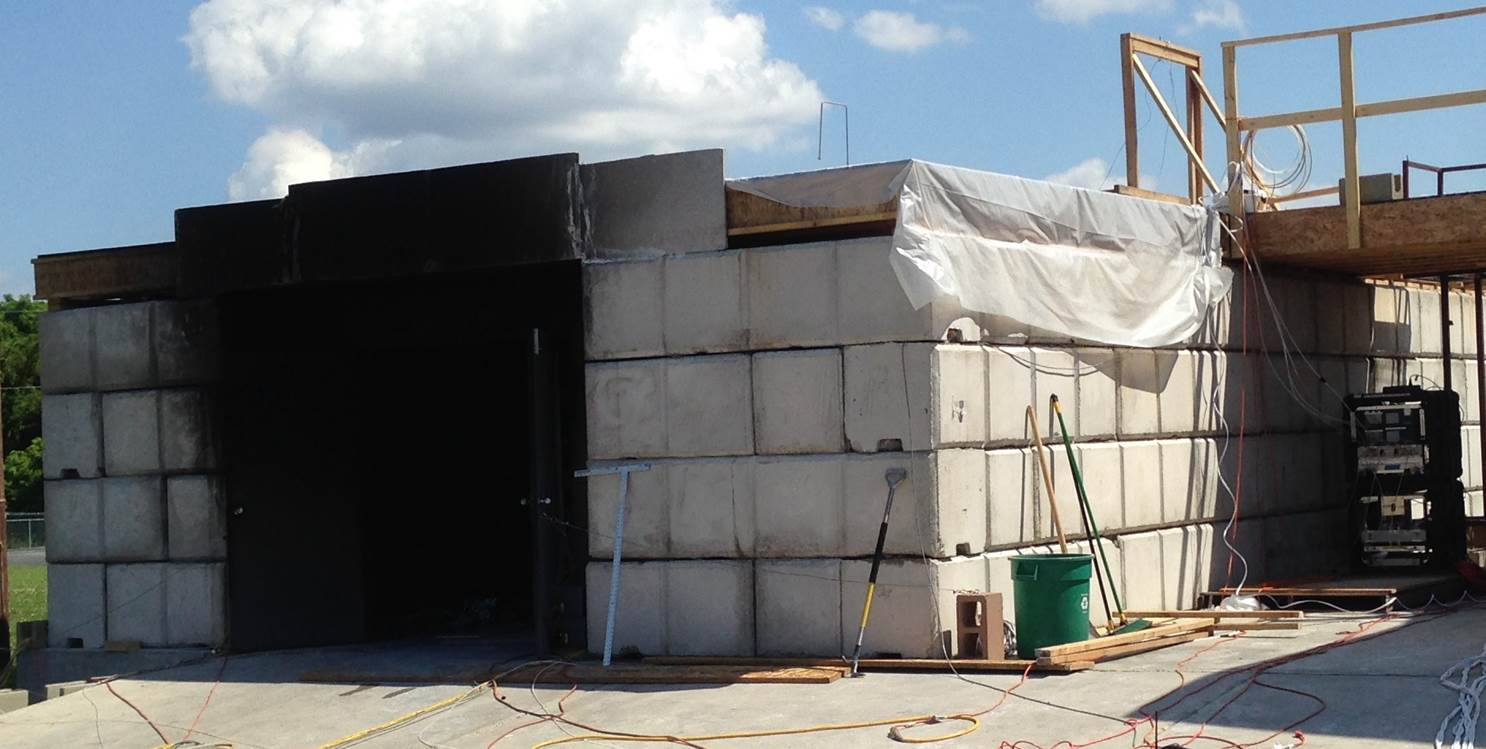
\includegraphics[width=5.25in]{../../Hose_Stream_Tests/Figures/Pictures/east_structure}
	\\~\\
	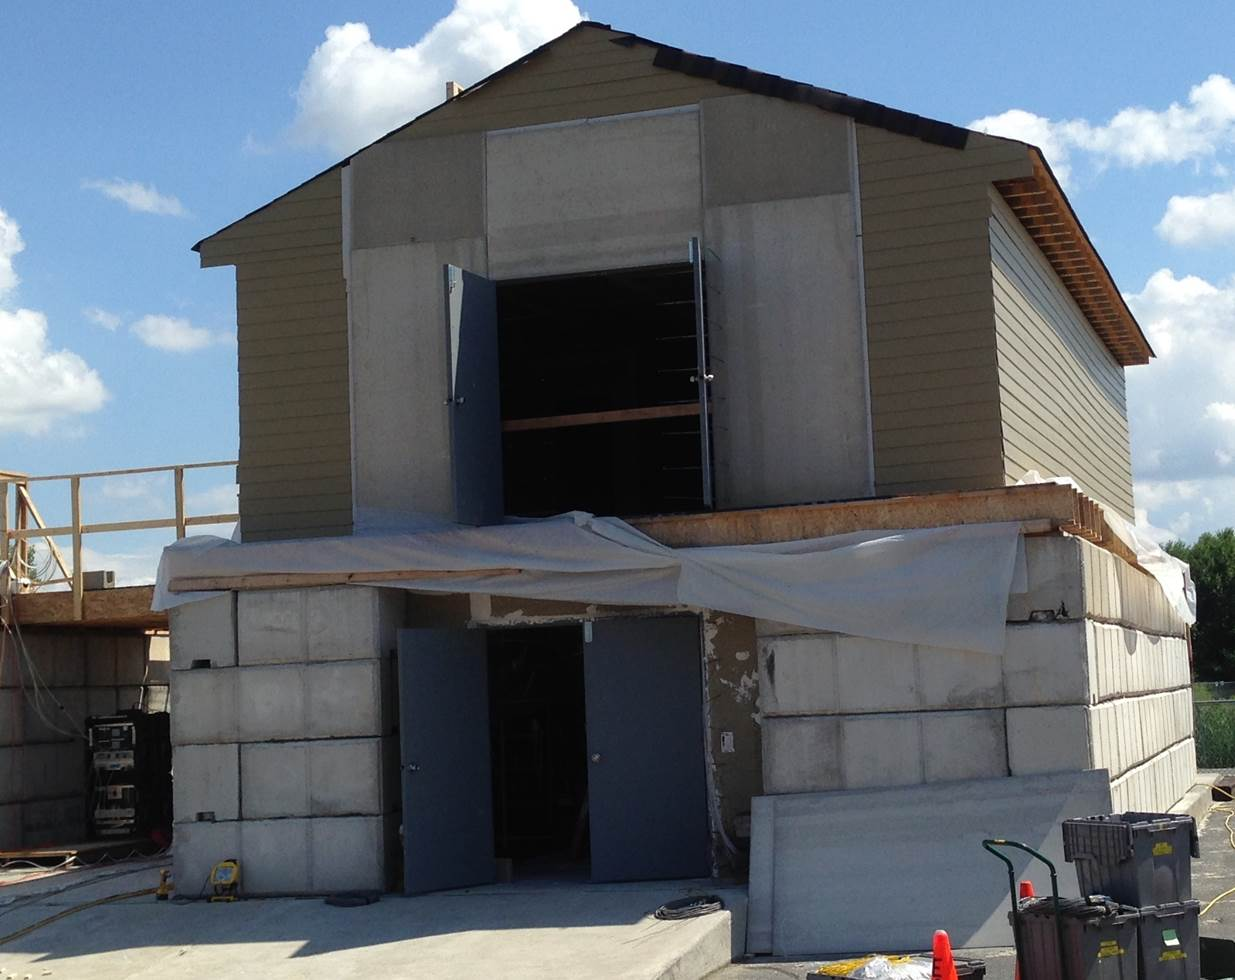
\includegraphics[width=5.25in]{../../Hose_Stream_Tests/Figures/Pictures/west_structure}
	\caption[North side of the East and West Structures.]{North side of the East Structure (top) and West Structure (bottom).}
	\label{fig:struct_pics}
\end{figure}

The interior walls of the first floor of each structure were framed with steel studs set to 400~mm (16~in) centers and track. Two layers of 16~mm (0.63~in) Type X gypsum board lined the steel studs, and a layer of 13~mm (0.5~in) thick cement board covered the gypsum board. Additionally, the ceiling was composed of two layers of 13~mm (0.5~in) thick cement board.
\FloatBarrier

The first floor ceiling support of each structure was composed of wood truss joist I-beams (TJIs) with a 298~mm (11.75~in) depth. Each TJI was composed of laminated veneer lumber flanges with a cross section of 29~mm (1.13~in) x 44~mm (1.75~in) and an 11~mm (0.43~in) thick oriented strand board web as shown in Fig.~\ref{fig:TJI}. Tongue and groove oriented strand board of 18.3~mm (0.72~in) thickness was screwed to the top of the TJIs.

\begin{figure}[!ht]
	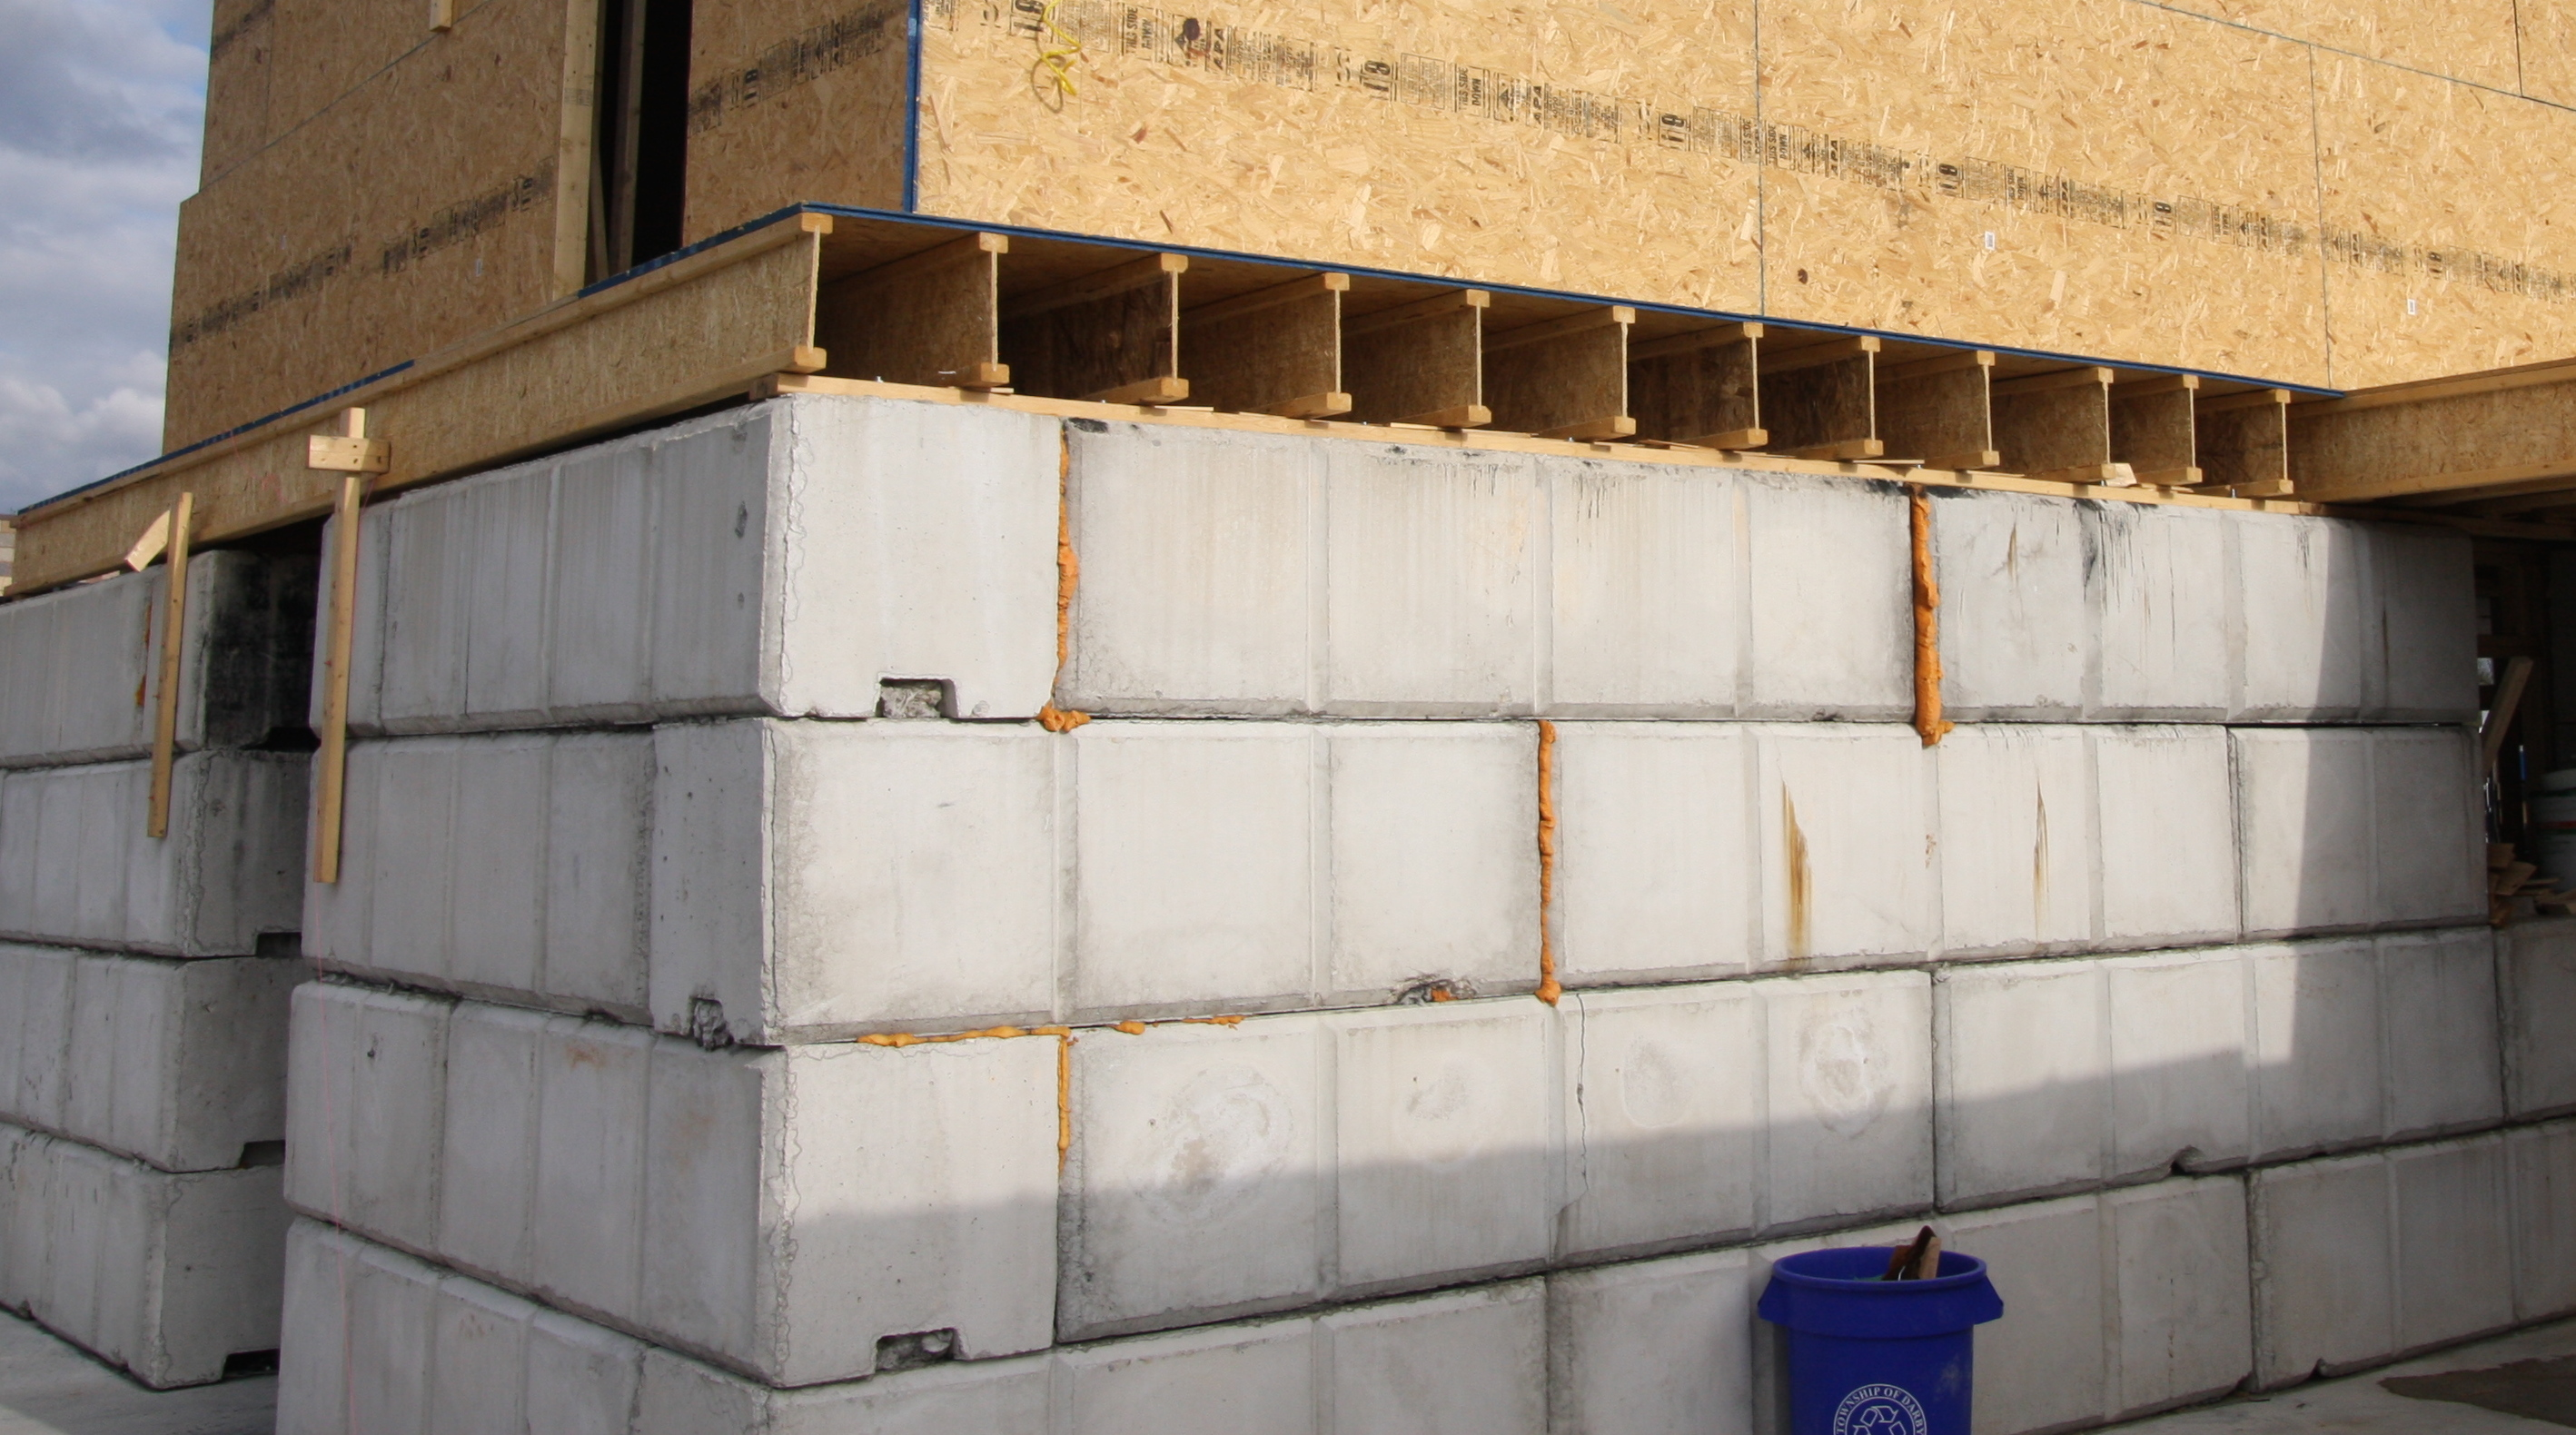
\includegraphics[width=6in]{../../Hose_Stream_Tests/Figures/Pictures/TJI_support}
	\caption[Ceiling support of the West Structure.]{First floor ceiling support of the West Structure composed of wood truss joist I-beams. View is of the southeast corner of the structure.}
	\label{fig:TJI}
\end{figure}
\FloatBarrier

\subsubsection{Second Floor of West Structure}
The second floor of the West Structure was built on the wood ceiling support described above and was connected to the first floor by a stairwell. The second story walls were of wood-frame with 51~mm (2~in) by 102~mm (4~in) studs set to 400~mm (16~in) centers. Two layers of 16~mm (0.63~in) Type X gypsum board lined the wood studs, and a layer of 13~mm (0.5~in) thick cement board covered the gypsum board. The exterior walls were protected with 11~mm (0.44~in) oriented strand board and 8~mm (0.31~in) fiber cement lap siding.

\subsection{Layout}
\label{sec:layout}

\subsubsection{Dimensions}
Dimensioned floor plans of the East and West Structures are presented in Figures~\ref{fig:east_dimensioned_plan}~and~\ref{fig:west_dimensioned_plan}, respectively.

\begin{figure}[!ht]
	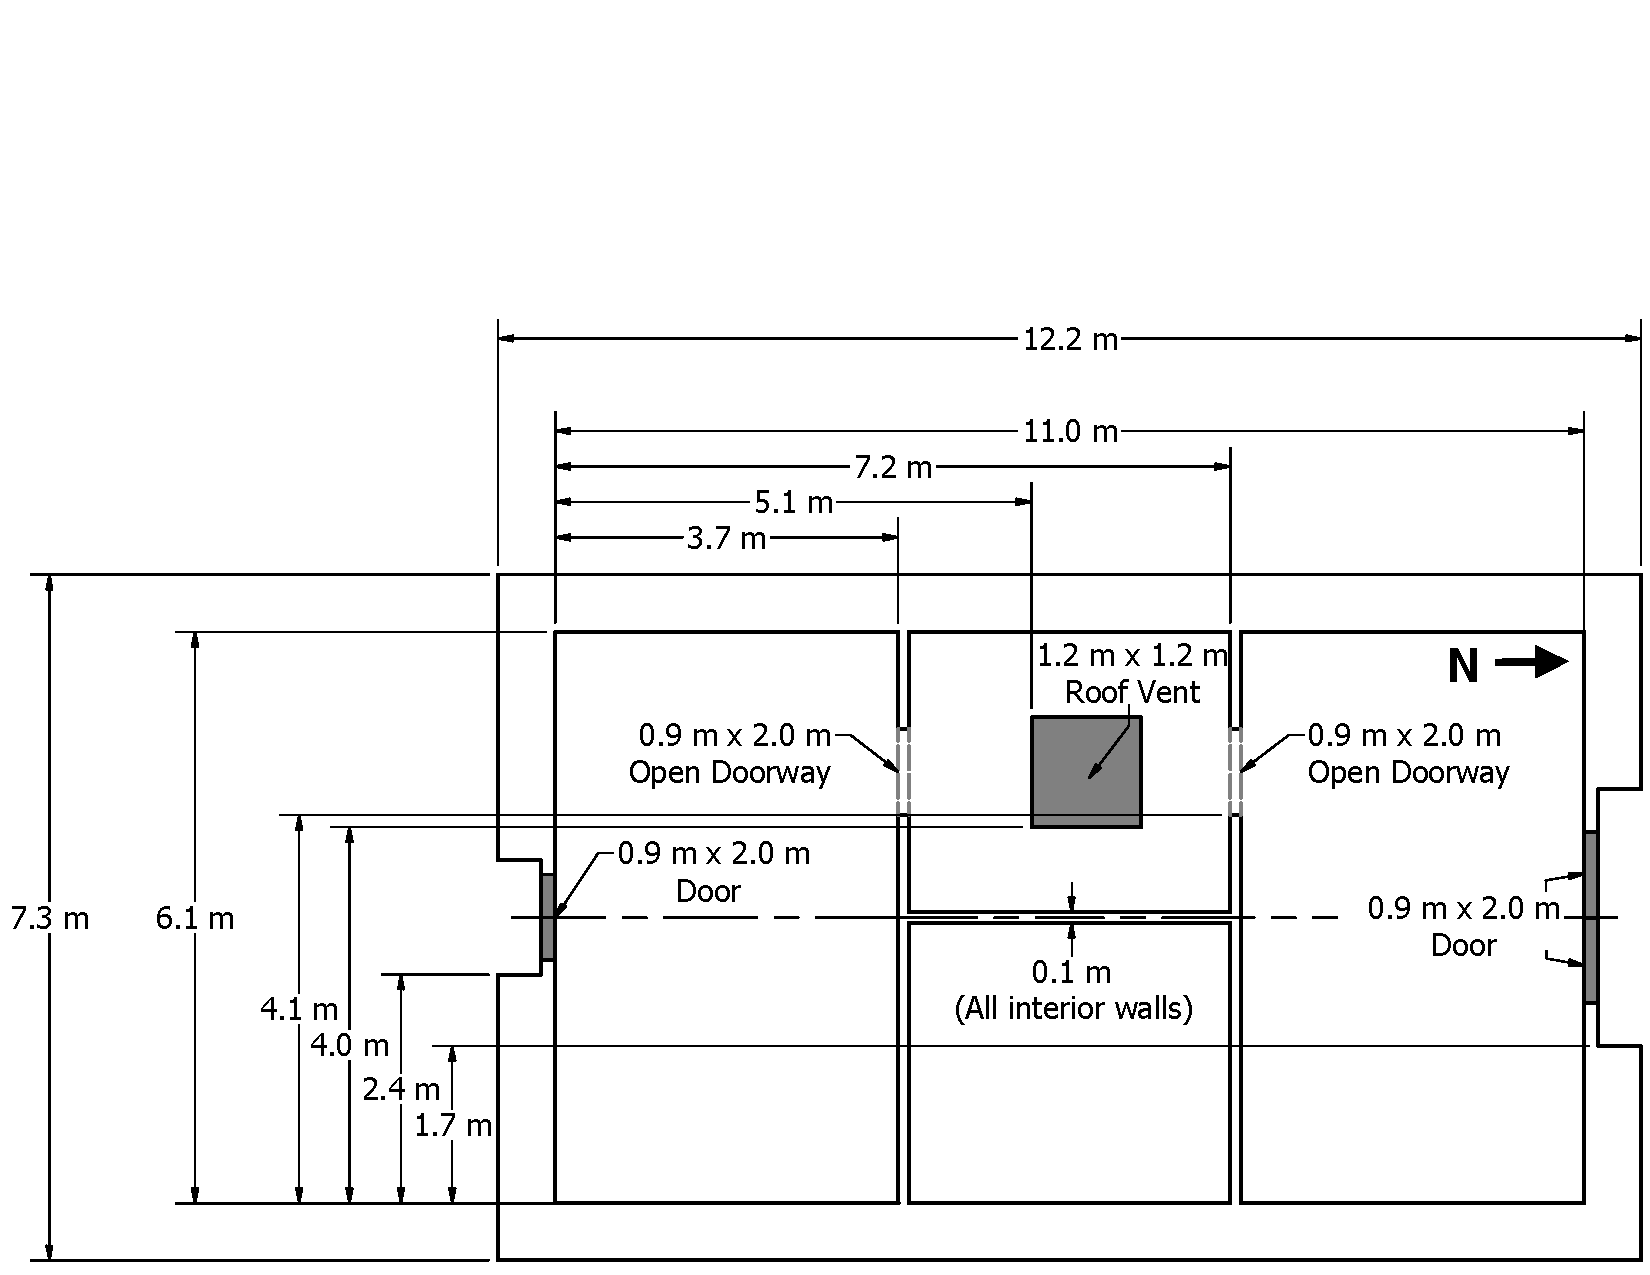
\includegraphics[width=\columnwidth]{../Figures/Floor_Plans/East_Structure_Dimensioned_Full}
	\caption[Dimensioned floor plan of the East Structure.]{Dimensioned floor plan of the East Structure. Structure dimensions are symmetric across horizontal centerline.}
	\label{fig:east_dimensioned_plan}
\end{figure}

\begin{figure}[!ht]
	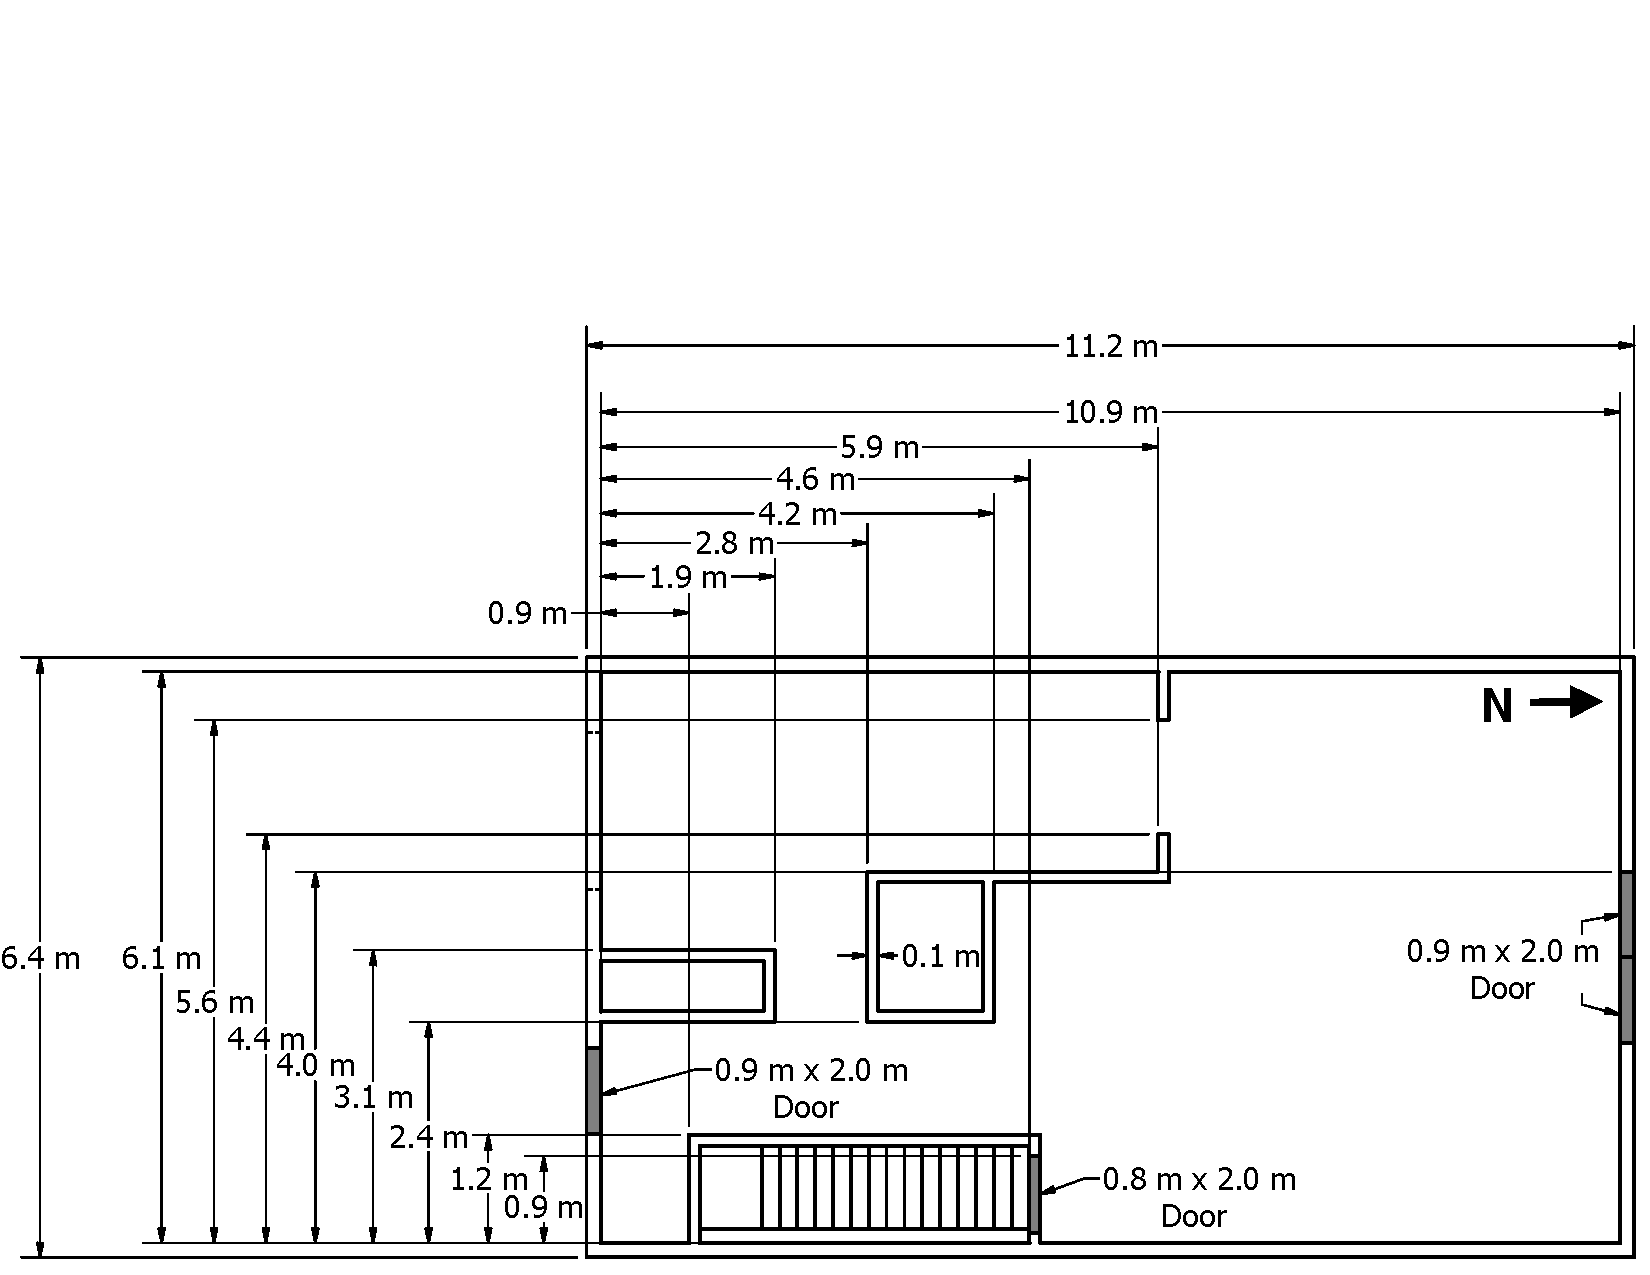
\includegraphics[width=\columnwidth]{../Figures/Floor_Plans/West_Structure_2nd_Floor_Dimensioned_Full}
	\\~\\
	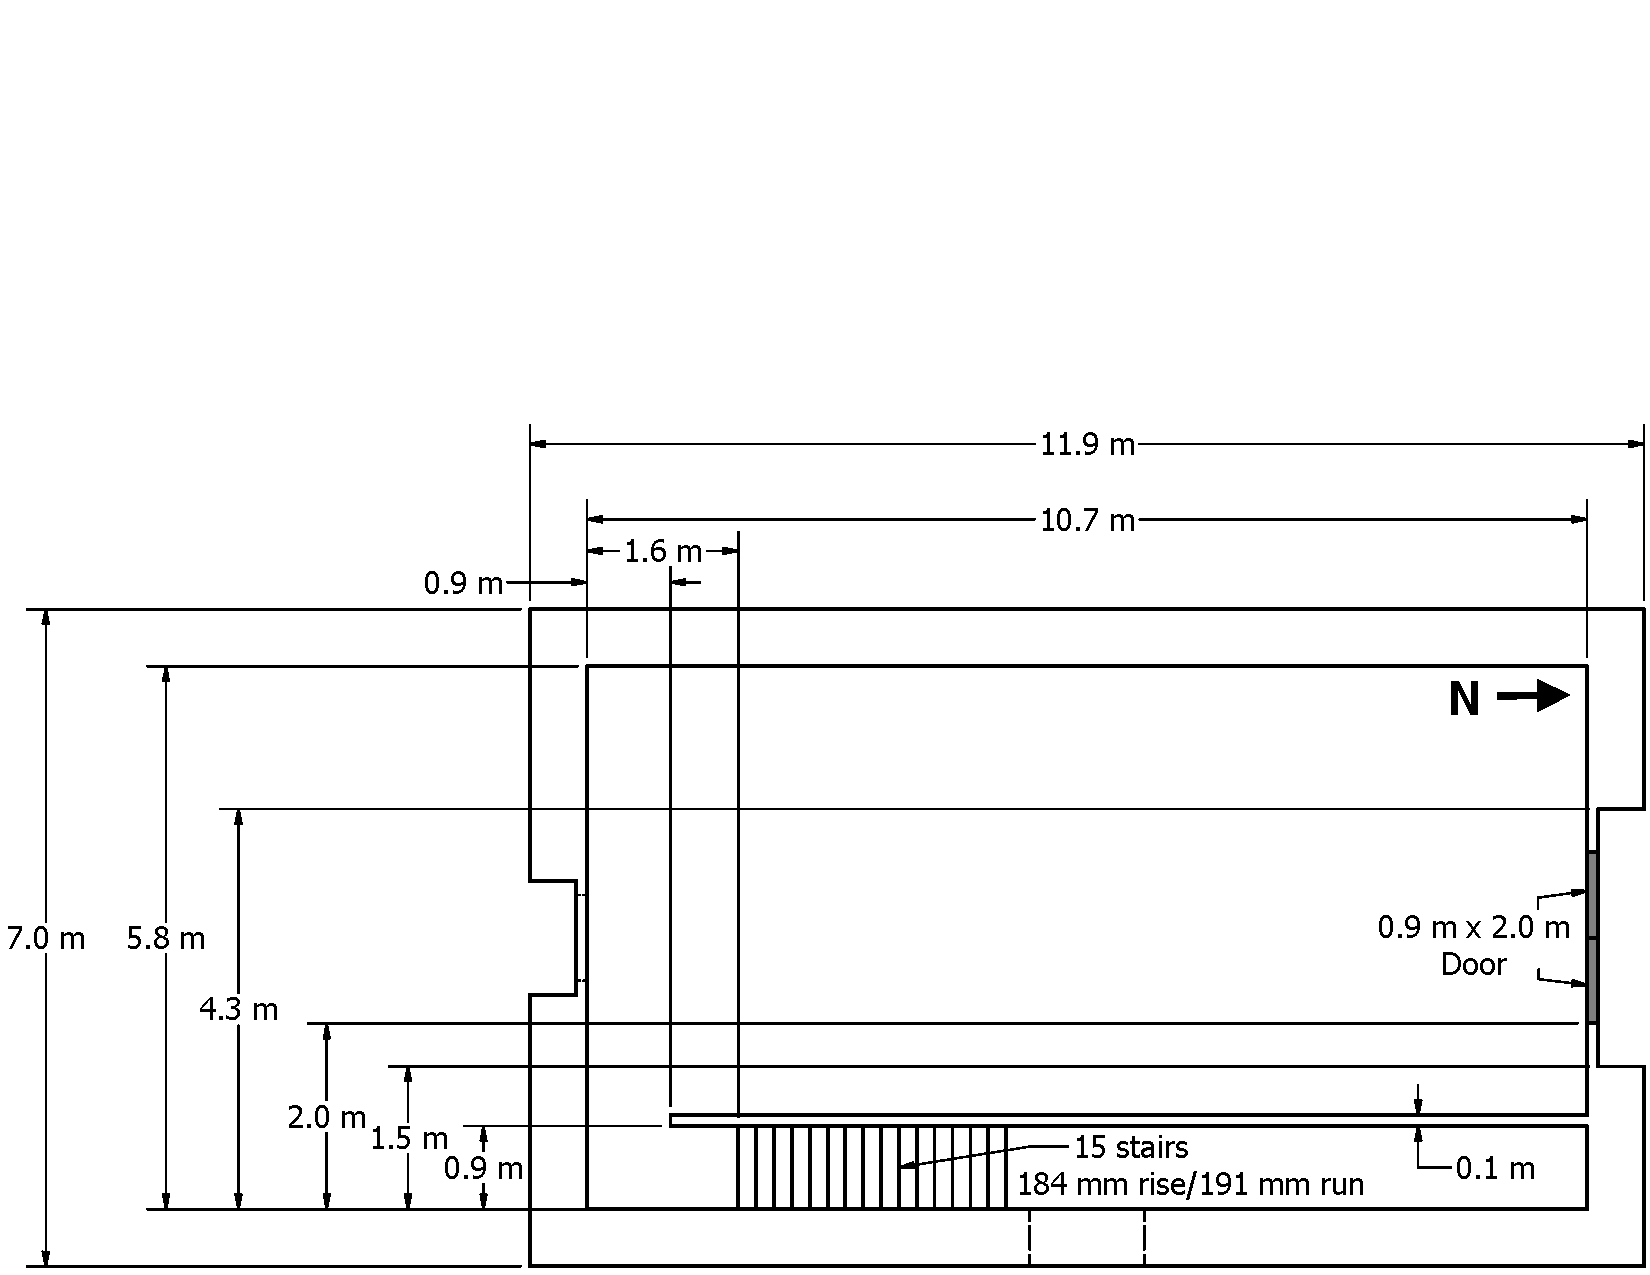
\includegraphics[width=\columnwidth]{../Figures/Floor_Plans/West_Structure_1st_Floor_Dimensioned_Full}
	\caption[Dimensioned floor plans of the West Structure.]{Dimensioned floor plan of the second floor (top) and first floor (bottom) of the West Structure.}
	\label{fig:west_dimensioned_plan}
\end{figure}

\FloatBarrier

The ceiling height of each structure was approximately 2.4~m (8~ft). The interior dimensions of the East Structure were approximately 6.1~m (20~ft) by 11~m (36~ft), and the interior dimensions of the first and second floors of the West Structure were 5.8~m (19~ft) by 10.7~m (35.1~ft) and 6.1~m (20~ft) by 10.9~m (35.8~ft), respectively. The stairs connecting the two floors of the West Structure started 1.6~m (5.3~ft) off the interior south wall with a width of 1.2~m (4~ft) off the interior east wall and contained a 184~mm (7.25~in) rise and 191~mm (7.5~in) run. The exterior doors of both structures, the stairwell door on the second level of the West Structure, and the square roof vent in the East Structure with a 1.2~m (4~ft) side length and 320~mm (12.75~in) depth were opened and closed at certain instances during experiments to change the ventilation patterns within the structures. The exterior doors were made of steel, and the stairwell door on the second level of the West Structure was made of lauan plywood. 
% The roof vent was composed of 16~mm (0.63~in) thick Type X gypsum board (interior side) attached to

\subsubsection{Leakage}
An air leakage measurement system was used to measure the amount of leakage associated with each structure. The amount of leakage in the East Structure was measured as 0.024~m$^2$. For the West Structure, the leakage was measured as 0.027~m$^2$ when the stairway door was closed and as 0.054~m$^2$ when the stairway door was opened.

\section{Instrumentation}
\label{sec:Instrumentation}
The structures were instrumented for temperature, gas velocity, heat flux, and gas concentration measurements. Gas temperatures in the burn rooms were measured with bare-bead, Chromel-Alumel (type K) thermocouples. Additional single thermocouples were installed in conjunction with bi-directional probes for gas velocity measurements. The single thermocouples were bare-bead, Chromel-Alumel (type K) thermocouples with a 1.0~mm (0.04~in) nominal diameter. The thermocouple wire was protected with a 3.2~mm (0.13~in) diameter inconel sheath. Schmidt-Boelter gauges were used to measure both total heat flux and radiant heat flux (radiometer). A radiometer is a total heat flux gauge with a zirconium plate to prevent contributions from convective heat transfer. Calibrated pumps pulled gas samples through a sample conditioning system to eliminate moisture in the sample. Then, the dry gas sample was piped to a series of gas analyzers and the concentrations of oxygen, carbon monoxide, and carbon dioxide were measured. A legend is presented in Fig.~\ref{fig:Instrumentation_Legend} to clarify the instrumentation schematics presented in the follow sections.

\begin{figure}[!ht]
	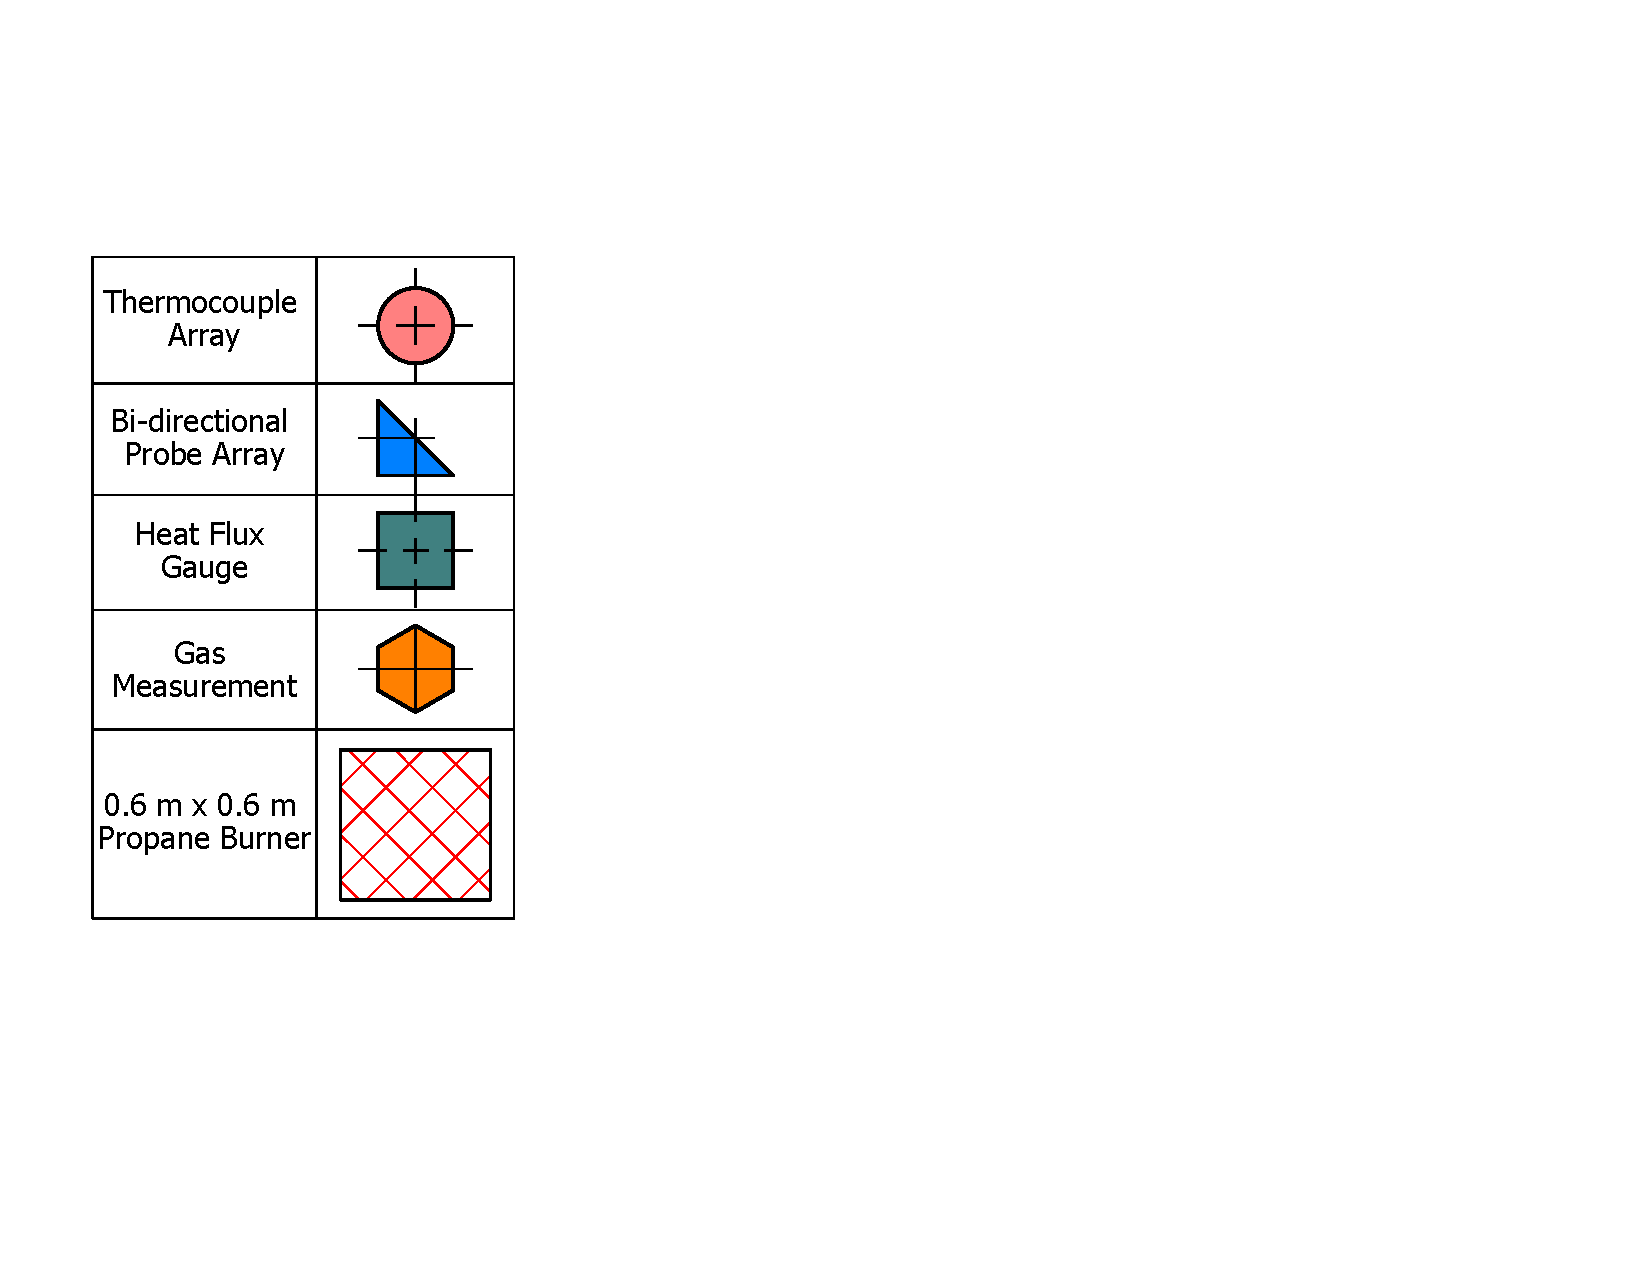
\includegraphics[width=0.25\columnwidth]{../Figures/Floor_Plans/Instrumentation_Legend}
	\caption[Instrumentation legend.]{Legend used for schematics of instrumentation locations.}
	\label{fig:Instrumentation_Legend}
\end{figure}

Three propane burners, pictured in Fig.~\ref{fig:burners}, were used as the fuel source in each experiment. Each burner had a square opening of side length 0.6~m (2~ft) located 0.14~m (5.5~in) above the floor and were positioned 0.6~m (2~ft) from the south and west walls on the first floor of each structure. Propane was supplied to the burners during all experiments. The flow of propane to each burner was controlled by a high-precision turn valve, and the total displaced gas volume was measured using a rotary gas meter.

\begin{figure}[!ht]
	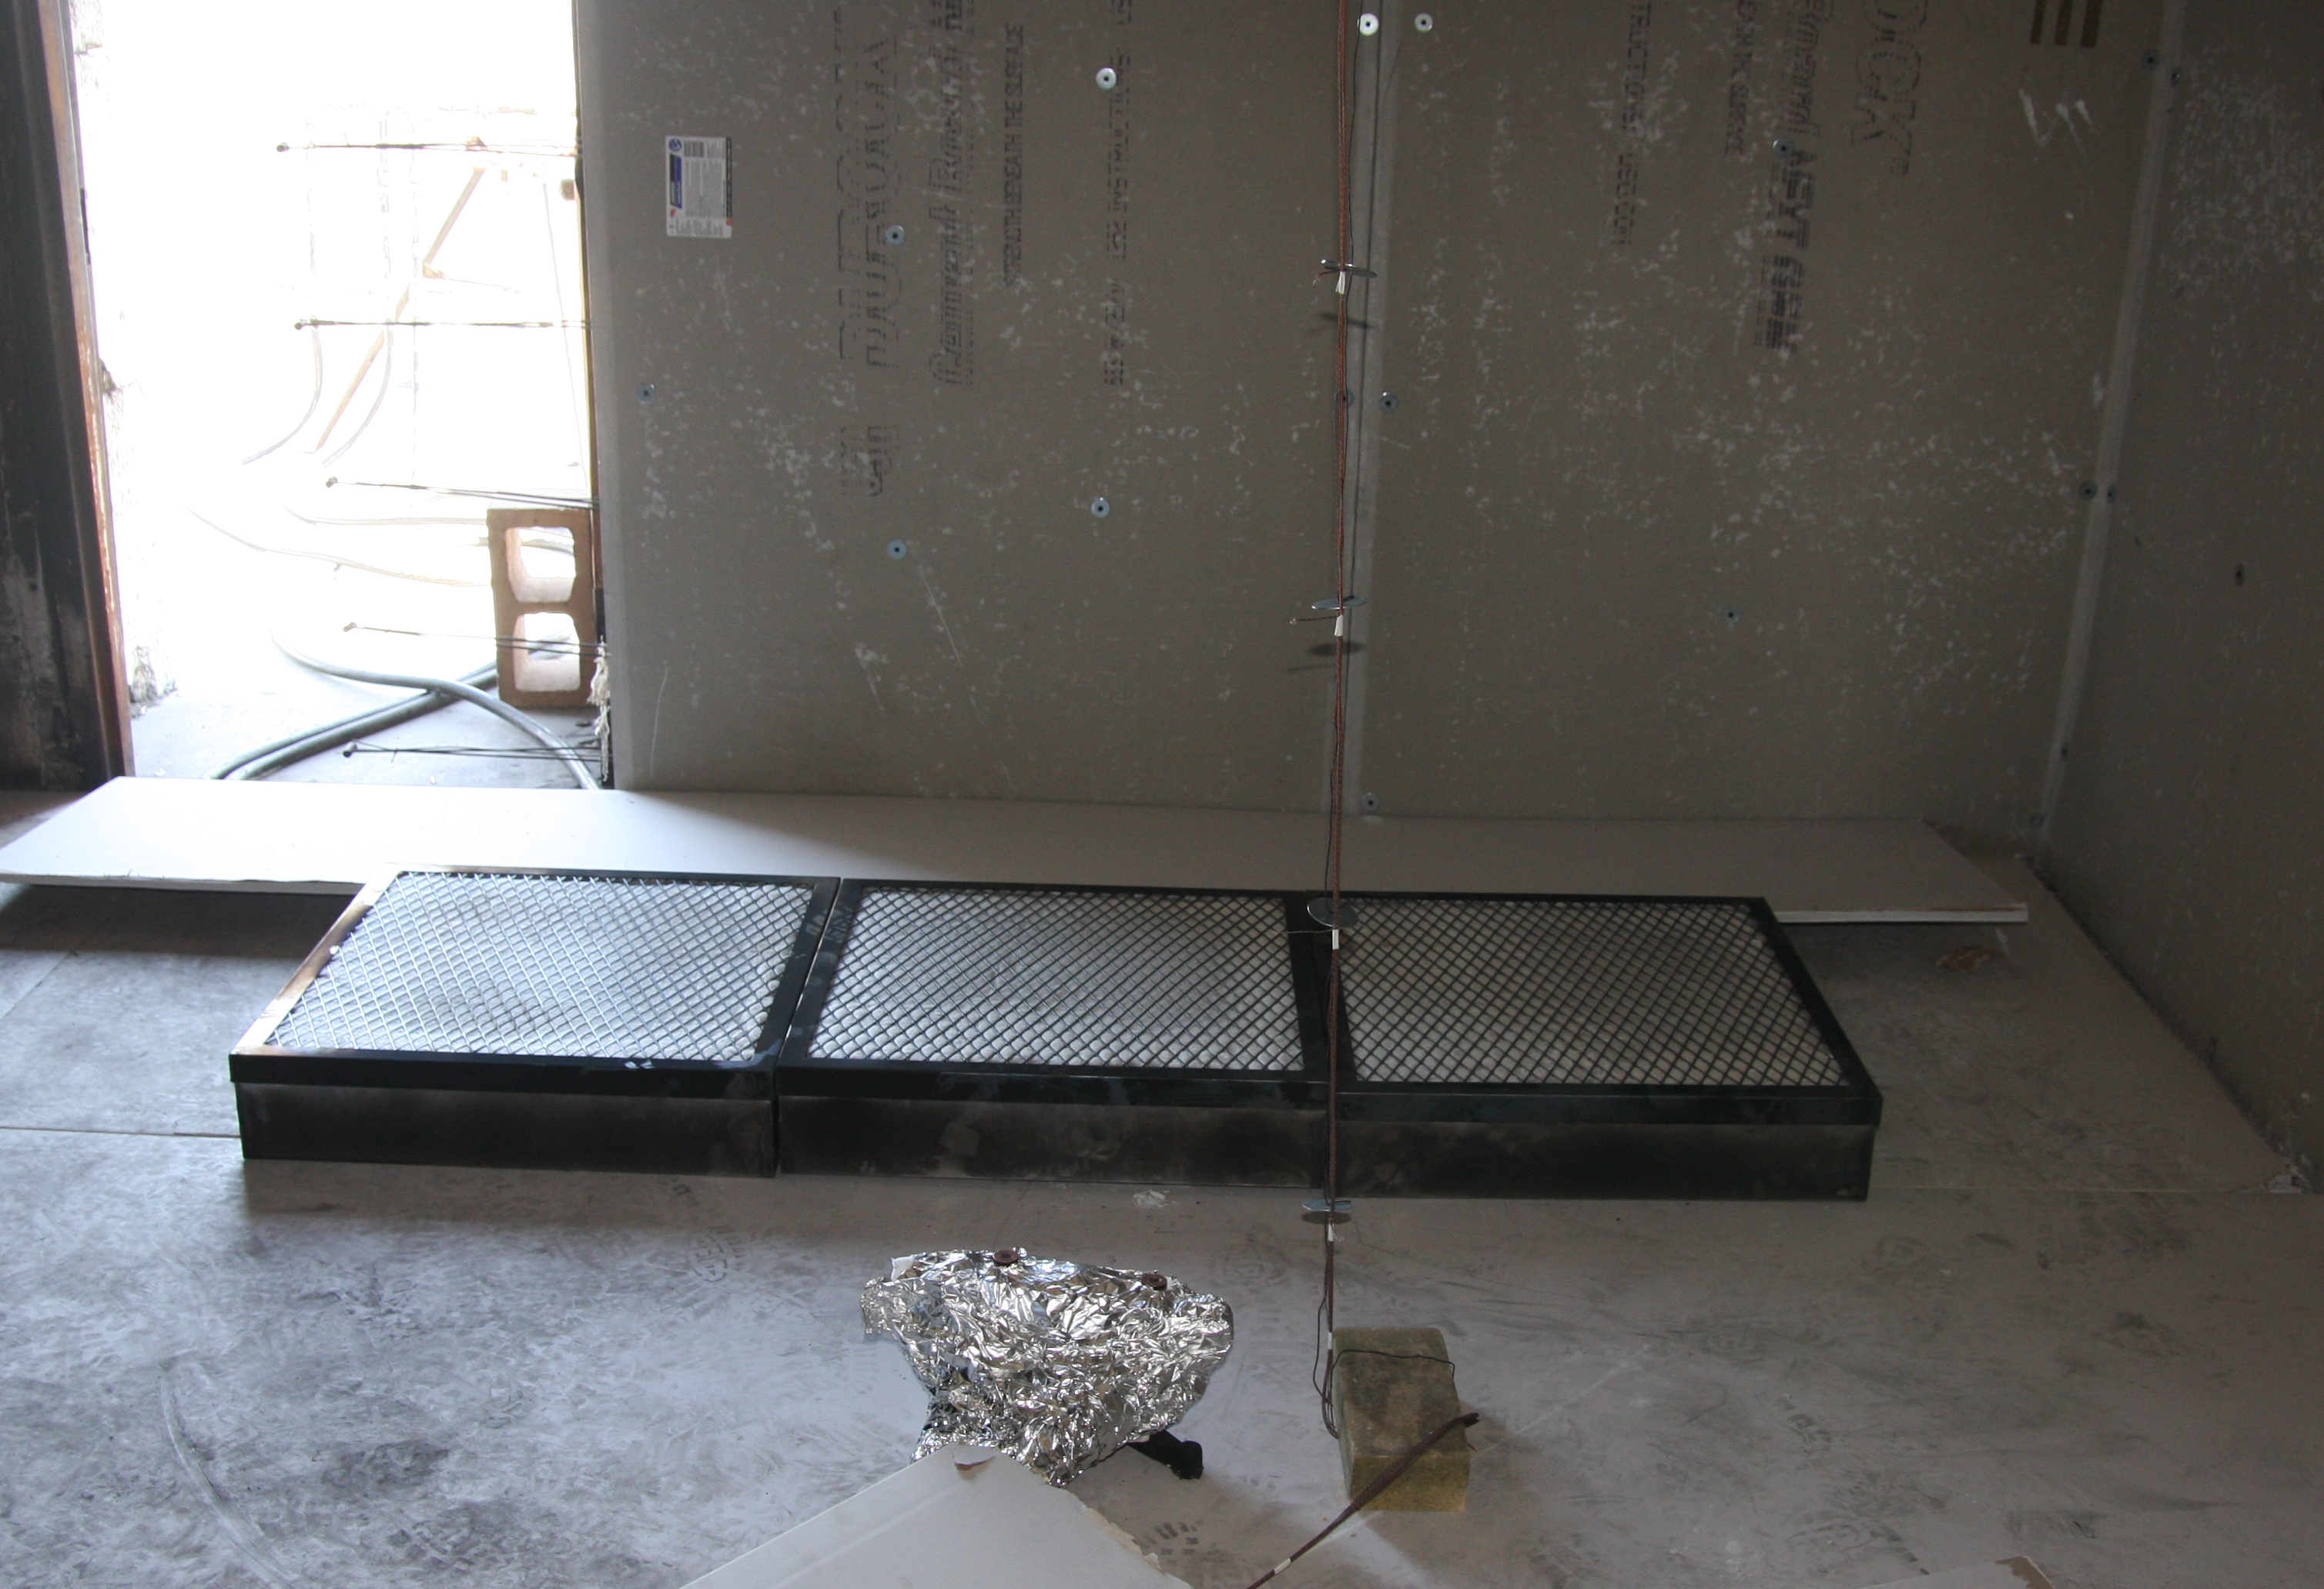
\includegraphics[width=0.9\columnwidth]{../Figures/Pictures/burners}
	\caption[Three propane burners used as fire source.]{Three propane burners located 0.6~m (2~ft) off the south and west interior walls on the first floor provided the fire source for the experiments.}
	\label{fig:burners}
\end{figure}

\FloatBarrier

\subsection{East Structure}
The East Structure was instrumented with five bare-bead thermocouple arrays, four bi-directional probe plus solid thermocouple arrays, five total heat flux plus radiometer sensor pairs, and two gas sample inlet pipes at the locations shown in Fig.~\ref{fig:east_instrumentation}.

\begin{figure}[!ht]
	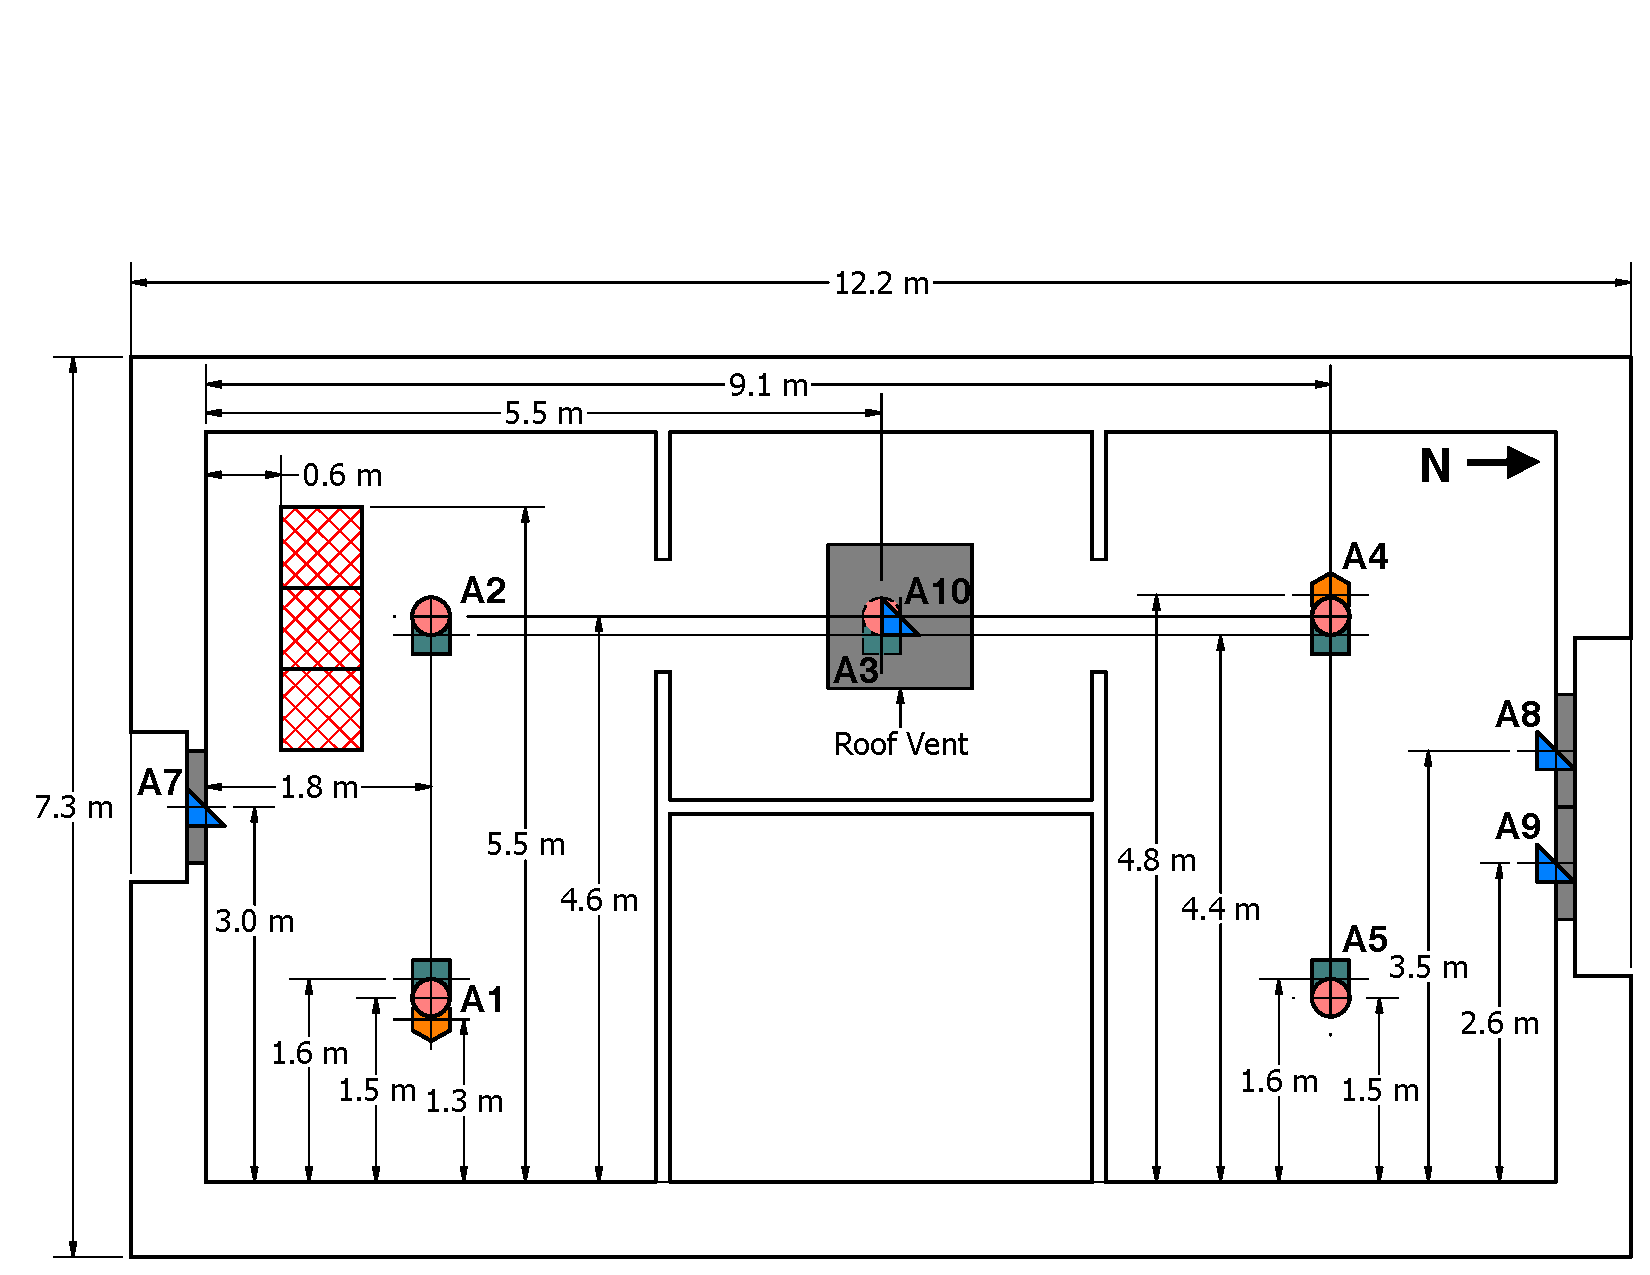
\includegraphics[width=\columnwidth]{../Figures/Floor_Plans/East_Structure_Dimensioned_Instrumentation}
	\caption{Locations and labels of instrumentation in the East Structure.}
	\label{fig:east_instrumentation}
\end{figure}
\FloatBarrier

Each bare-bead thermocouple array was composed of eight thermocouples. Three bi-directional probe and solid thermocouple arrays (A7, A8, and A9) were centered in each exterior doorway of the structure and contained eight probes as shown in Fig.~\ref{fig:BDP_arrays}. The fourth bi-directional probe and solid thermocouple array (A10), also presented in Fig.~\ref{fig:BDP_arrays}, was located at the opening of the roof vent and contained three probes centered between the east and west sides of the vent. The position of each probe and thermocouple pair relative to the south wall of the vent are listed in Table~\ref{table:east_channel_list}. The total heat flux gauge/radiometer pairs were set to be aimed to view the ceiling. Gas concentrations were pulled through 9.5~mm (0.38~in) diameter stainless steel tubing. The height of each individual sensor in the sensor arrays are listed in the channel list found in Table~\ref{table:east_channel_list}.   

\begin{figure}[!ht]
	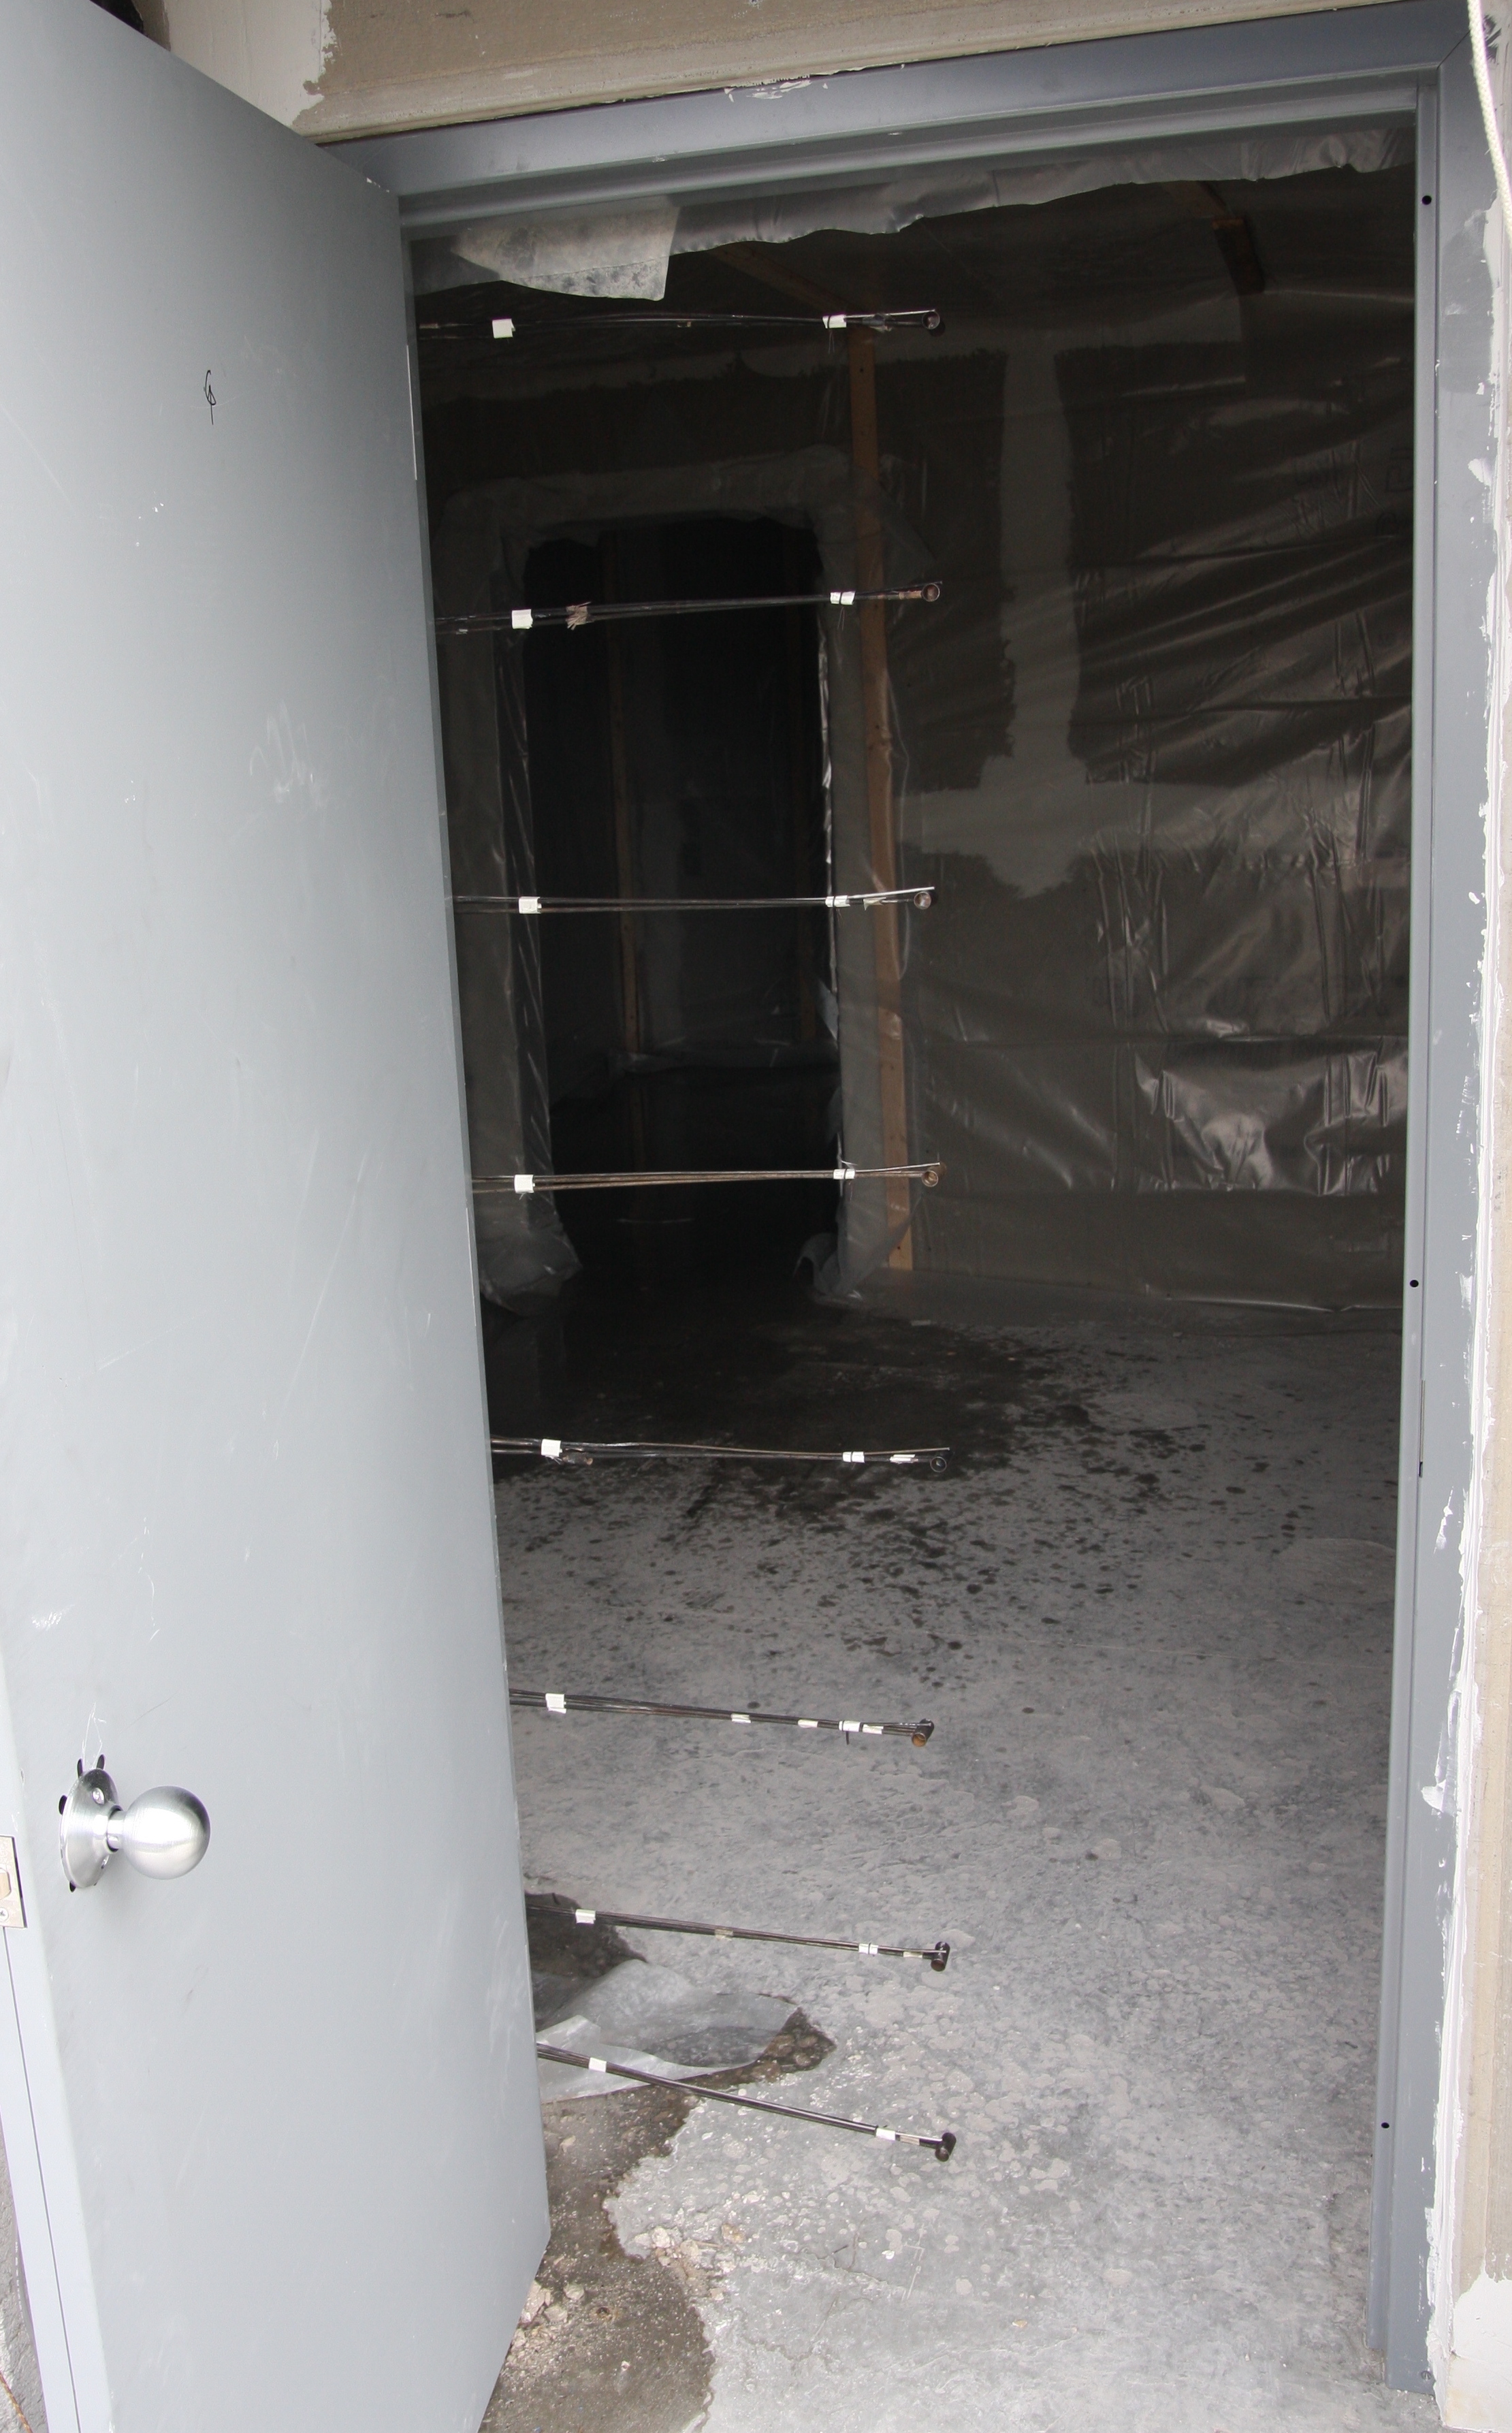
\includegraphics[width=0.45\columnwidth]{../Figures/Pictures/doorway_BDPs}
	\\~\\
	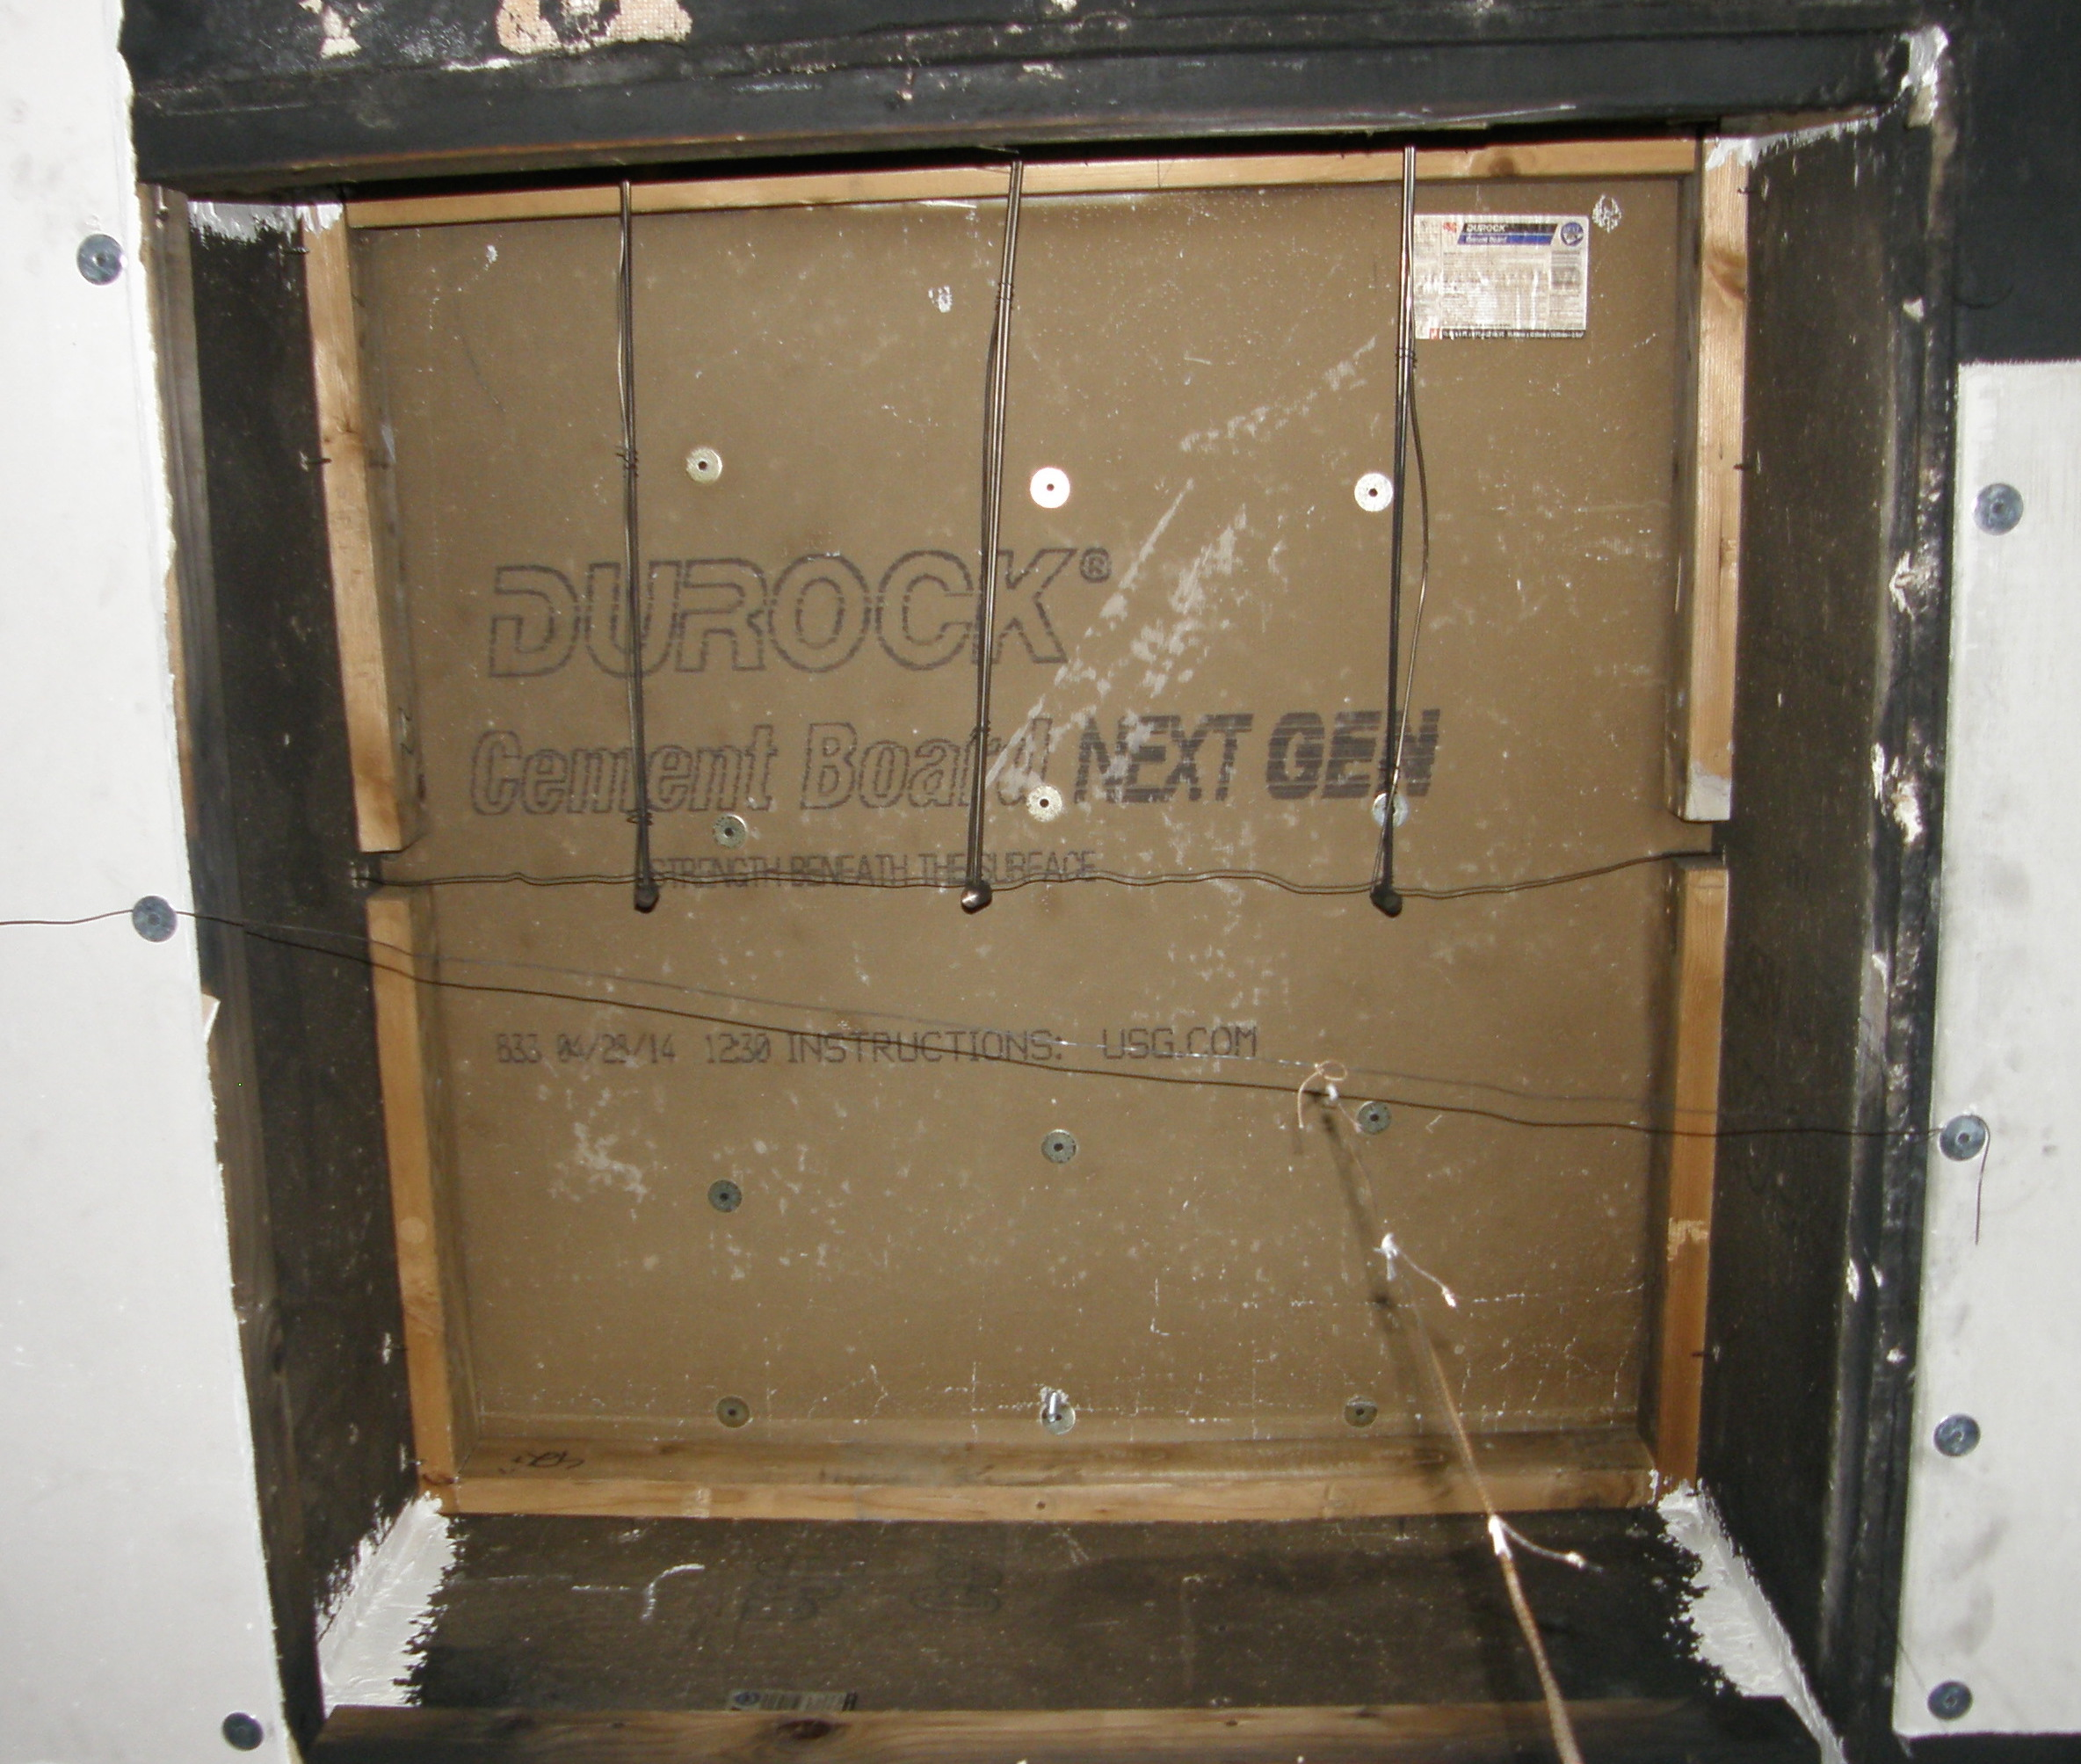
\includegraphics[width=0.65\columnwidth]{../Figures/Pictures/roof_vent_BDPs}
	\caption[Bi-directional probe plus solid thermocouple arrays in East Structure.]{Bi-directional probe plus solid thermocouple array at the south exterior doorway (top) and roof vent (bottom) of the East Structure.}
	\label{fig:BDP_arrays}
\end{figure}

\clearpage

\begin{longtable}[c]{c|lll}
\caption{East Structure Channel List\label{table:east_channel_list}} \\
\toprule
\begin{tabular}{c} \textbf{Device} \\ \textbf{Location} \end{tabular} & 
\begin{tabular}{c} \textbf{Channel} \\ \textbf{Name} \end{tabular}  & 
\textbf{Channel Location} & 
\textbf{Measurement Type} \\
\midrule
\endhead
\multirow{13}{*}{\large\textbf{A1}} 
 & TC\_A1\_1  & 0.03~m below ceiling & Temperature \\
 & TC\_A1\_2  & 0.30~m below ceiling & Temperature \\
 & TC\_A1\_3  & 0.61~m below ceiling & Temperature \\
 & TC\_A1\_4  & 0.91~m below ceiling & Temperature \\
 & TC\_A1\_5  & 1.22~m below ceiling & Temperature \\
 & TC\_A1\_6  & 1.52~m below ceiling & Temperature \\
 & TC\_A1\_7  & 1.83~m below ceiling & Temperature \\
 & TC\_A1\_8  & 2.13~m below ceiling & Temperature \\
\cline{2-4}
 & HF\_A1	  & 0.15~m above floor   & Total heat flux \\
 & RAD\_A1    & 0.15~m above floor   & Radiative heat flux \\
\cline{2-4}
 & CO\_A      & 1.22~m above floor   & CO concentration \\
 & CO2\_A     & 1.22~m above floor   & CO$_2$ concentration \\
 & O2\_A      & 1.22~m above floor   & O$_2$ concentration \\
\midrule
\multirow{10}{*}{\large{\textbf{A2}}}
 & TC\_A2\_1  & 0.03~m below ceiling & Temperature \\
 & TC\_A2\_2  & 0.30~m below ceiling & Temperature \\
 & TC\_A2\_3  & 0.61~m below ceiling & Temperature \\
 & TC\_A2\_4  & 0.91~m below ceiling & Temperature \\
 & TC\_A2\_5  & 1.22~m below ceiling & Temperature \\
 & TC\_A2\_6  & 1.52~m below ceiling & Temperature \\
 & TC\_A2\_7  & 1.83~m below ceiling & Temperature \\
 & TC\_A2\_8  & 2.13~m below ceiling & Temperature \\
\cline{2-4}
 & HF\_A2	  & 0.15~m above floor   & Total heat flux \\
 & RAD\_A2    & 0.15~m above floor   & Radiative heat flux \\
\midrule
 \multirow{10}{*}{\large{\textbf{A3}}}
 & TC\_A3\_1  & 0.03~m below ceiling & Temperature \\
 & TC\_A3\_2  & 0.30~m below ceiling & Temperature \\
 & TC\_A3\_3  & 0.61~m below ceiling & Temperature \\
 & TC\_A3\_4  & 0.91~m below ceiling & Temperature \\
 & TC\_A3\_5  & 1.22~m below ceiling & Temperature \\
 & TC\_A3\_6  & 1.52~m below ceiling & Temperature \\
 & TC\_A3\_7  & 1.83~m below ceiling & Temperature \\
 & TC\_A3\_8  & 2.13~m below ceiling & Temperature \\
\cline{2-4}
 & HF\_A3	  & 0.15~m above floor   & Total heat flux \\
 & RAD\_A3    & 0.15~m above floor   & Radiative heat flux \\
% \midrule
\bottomrule
\newpage
\multirow{13}{*}{\large\textbf{A4}} 
 & TC\_A4\_1  & 0.03~m below ceiling & Temperature \\
 & TC\_A4\_2  & 0.30~m below ceiling & Temperature \\
 & TC\_A4\_3  & 0.61~m below ceiling & Temperature \\
 & TC\_A4\_4  & 0.91~m below ceiling & Temperature \\
 & TC\_A4\_5  & 1.22~m below ceiling & Temperature \\
 & TC\_A4\_6  & 1.52~m below ceiling & Temperature \\
 & TC\_A4\_7  & 1.83~m below ceiling & Temperature \\
 & TC\_A4\_8  & 2.13~m below ceiling & Temperature \\
\cline{2-4}
 & HF\_A4	  & 0.15~m above floor   & Total heat flux \\
 & RAD\_A4    & 0.15~m above floor   & Radiative heat flux \\
\cline{2-4}
 & CO\_B      & 1.22~m above floor   & CO concentration \\
 & CO2\_B     & 1.22~m above floor   & CO$_2$ concentration \\
 & O2\_B      & 1.22~m above floor   & O$_2$ concentration \\
\midrule
\multirow{10}{*}{\large{\textbf{A5}}}
 & TC\_A5\_1  & 0.03~m below ceiling & Temperature \\
 & TC\_A5\_2  & 0.30~m below ceiling & Temperature \\
 & TC\_A5\_3  & 0.61~m below ceiling & Temperature \\
 & TC\_A5\_4  & 0.91~m below ceiling & Temperature \\
 & TC\_A5\_5  & 1.22~m below ceiling & Temperature \\
 & TC\_A5\_6  & 1.52~m below ceiling & Temperature \\
 & TC\_A5\_7  & 1.83~m below ceiling & Temperature \\
 & TC\_A5\_8  & 2.13~m below ceiling & Temperature \\
\cline{2-4}
 & HF\_A5	  & 0.15~m above floor   & Total heat flux \\
 & RAD\_A5    & 0.15~m above floor   & Radiative heat flux \\
\midrule
\multirow{16}{*}{\large{\textbf{A7}}}
 & TC\_A7\_1  & 0.08~m below soffit  & Temperature \\
 & TC\_A7\_2  & 0.34~m below soffit  & Temperature \\
 & TC\_A7\_3  & 0.61~m below soffit  & Temperature \\
 & TC\_A7\_4  & 0.88~m below soffit  & Temperature \\
 & TC\_A7\_5  & 1.15~m below soffit  & Temperature \\
 & TC\_A7\_6  & 1.42~m below soffit  & Temperature \\
 & TC\_A7\_7  & 1.68~m below soffit  & Temperature \\
 & TC\_A7\_8  & 1.95~m below soffit  & Temperature \\
\cline{2-4}
 & BDP\_A7\_1 & 0.08~m below soffit  & Velocity \\
 & BDP\_A7\_2 & 0.34~m below soffit  & Velocity \\
 & BDP\_A7\_3 & 0.61~m below soffit  & Velocity \\
 & BDP\_A7\_4 & 0.88~m below soffit  & Velocity \\
 & BDP\_A7\_5 & 1.15~m below soffit  & Velocity \\
 & BDP\_A7\_6 & 1.42~m below soffit  & Velocity \\
 & BDP\_A7\_7 & 1.68~m below soffit  & Velocity \\
 & BDP\_A7\_8 & 1.95~m below soffit  & Velocity \\
\bottomrule
\newpage
\multirow{16}{*}{\large{\textbf{A8}}}
 & TC\_A8\_1  & 0.08~m below soffit  & Temperature \\
 & TC\_A8\_2  & 0.34~m below soffit  & Temperature \\
 & TC\_A8\_3  & 0.61~m below soffit  & Temperature \\
 & TC\_A8\_4  & 0.88~m below soffit  & Temperature \\
 & TC\_A8\_5  & 1.15~m below soffit  & Temperature \\
 & TC\_A8\_6  & 1.42~m below soffit  & Temperature \\
 & TC\_A8\_7  & 1.68~m below soffit  & Temperature \\
 & TC\_A8\_8  & 1.95~m below soffit  & Temperature \\
\cline{2-4}
 & BDP\_A8\_1 & 0.08~m below soffit  & Velocity \\
 & BDP\_A8\_2 & 0.34~m below soffit  & Velocity \\
 & BDP\_A8\_3 & 0.61~m below soffit  & Velocity \\
 & BDP\_A8\_4 & 0.88~m below soffit  & Velocity \\
 & BDP\_A8\_5 & 1.15~m below soffit  & Velocity \\
 & BDP\_A8\_6 & 1.42~m below soffit  & Velocity \\
 & BDP\_A8\_7 & 1.68~m below soffit  & Velocity \\
 & BDP\_A8\_8 & 1.95~m below soffit  & Velocity \\
\midrule
\multirow{16}{*}{\large{\textbf{A9}}}
 & TC\_A9\_1  & 0.08~m below soffit  & Temperature \\
 & TC\_A9\_2  & 0.34~m below soffit  & Temperature \\
 & TC\_A9\_3  & 0.61~m below soffit  & Temperature \\
 & TC\_A9\_4  & 0.88~m below soffit  & Temperature \\
 & TC\_A9\_5  & 1.15~m below soffit  & Temperature \\
 & TC\_A9\_6  & 1.42~m below soffit  & Temperature \\
 & TC\_A9\_7  & 1.68~m below soffit  & Temperature \\
 & TC\_A9\_8  & 1.95~m below soffit  & Temperature \\
\cline{2-4}
 & BDP\_A9\_1 & 0.08~m below soffit  & Velocity \\
 & BDP\_A9\_2 & 0.34~m below soffit  & Velocity \\
 & BDP\_A9\_3 & 0.61~m below soffit  & Velocity \\
 & BDP\_A9\_4 & 0.88~m below soffit  & Velocity \\
 & BDP\_A9\_5 & 1.15~m below soffit  & Velocity \\
 & BDP\_A9\_6 & 1.42~m below soffit  & Velocity \\
 & BDP\_A9\_7 & 1.68~m below soffit  & Velocity \\
 & BDP\_A9\_8 & 1.95~m below soffit  & Velocity \\
\midrule
\multirow{6}{*}{\large{\textbf{A10}}}
 & TC\_A10\_1 & 0.91~m from S side of vent & Temperature \\
 & TC\_A10\_2 & 0.61~m from S side of vent & Temperature \\
 & TC\_A10\_3 & 0.30~m from S side of vent & Temperature \\
\cline{2-4}
 & BDP\_A10\_1 & 0.91~m from S side of vent & Velocity \\
 & BDP\_A10\_2 & 0.61~m from S side of vent & Velocity \\
 & BDP\_A10\_3 & 0.30~m from S side of vent & Velocity \\
\bottomrule
\end{longtable}
\clearpage

\subsection{West Structure}
The first floor of the West Structure was instrumented with three bare-bead thermocouple arrays, two bi-directional probe plus solid thermocouple arrays, and one gas sample inlet pipe. The second floor was equipped with three bare-bead thermocouple arrays, four bi-directional probe plus solid thermocouple arrays, two total heat flux sensor pairs, and one gas sample inlet pipe. The location of the instrumentation in the West Structure is shown in Fig.~\ref{fig:west_instrumentation}.

\begin{figure}[!ht]
	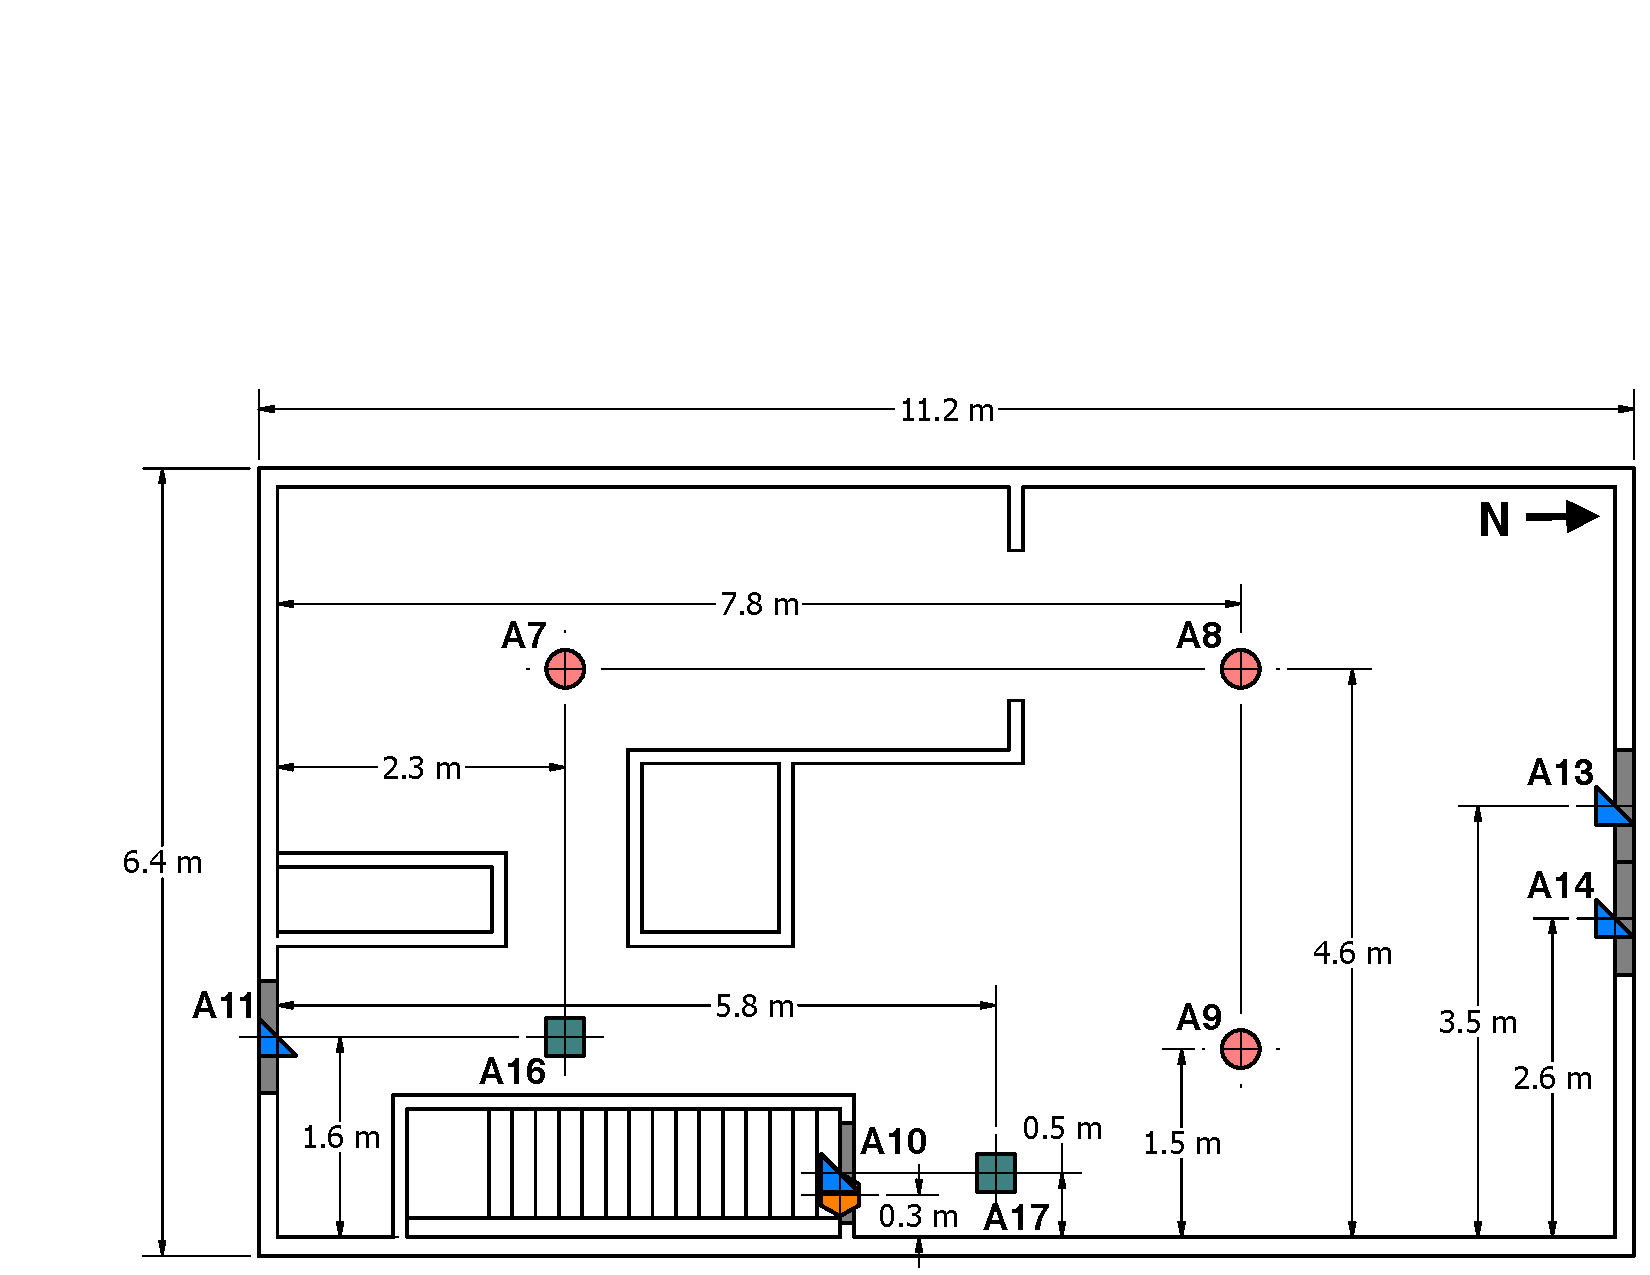
\includegraphics[width=0.94\columnwidth]{../Figures/Floor_Plans/West_Structure_2nd_Floor_Dimensioned_Instrumentation}
	\\~\\
	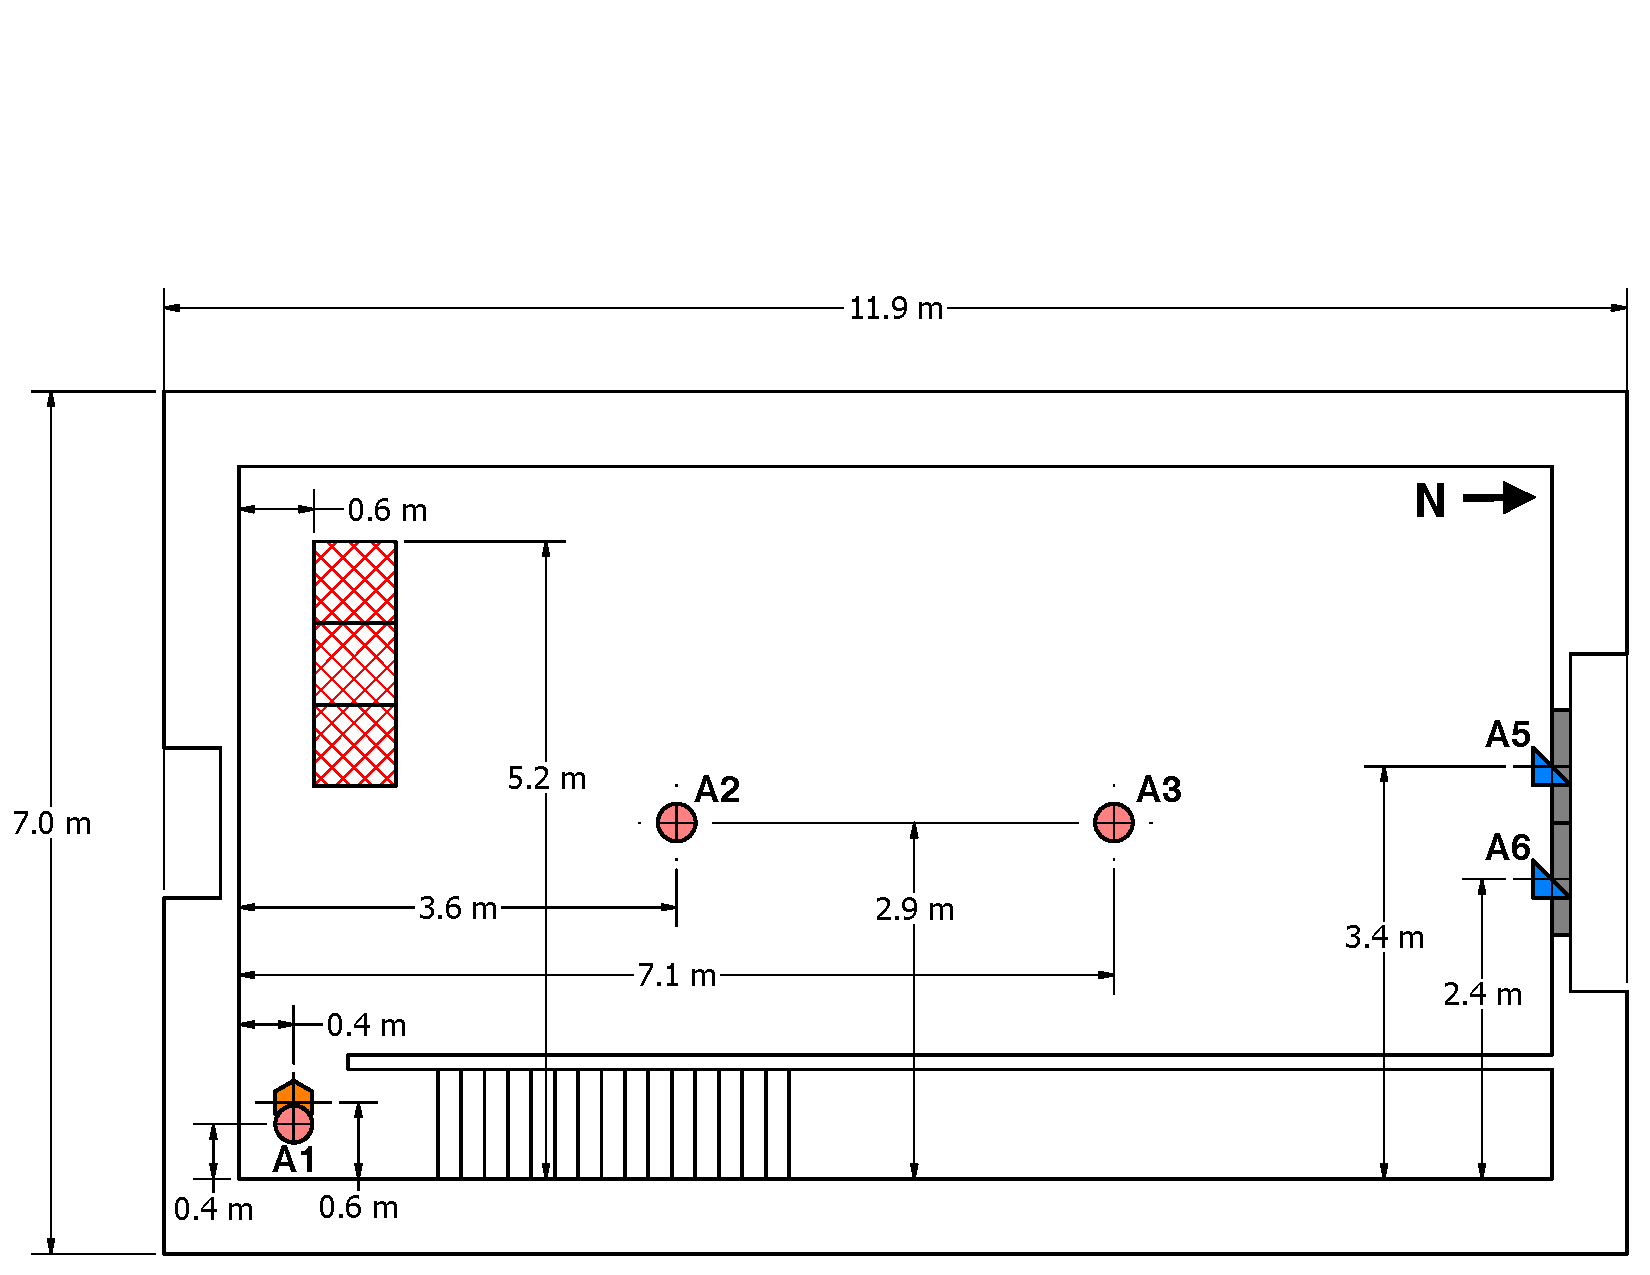
\includegraphics[width=\columnwidth]{../Figures/Floor_Plans/West_Structure_1st_Floor_Dimensioned_Instrumentation}
	\caption[Locations and labels of instrumentation in the West Structure.]{Locations and labels of instrumentation in the second floor (top) and first floor (bottom) of the West Structure.}
	\label{fig:west_instrumentation}
\end{figure}

Every thermocouple array contained eight bare-bead thermocouples, each bi-directional probe and solid thermocouple array contained 8 probes, and gas concentrations were pulled through 9.5~mm (0.38~in) diameter stainless steel tubing located 1.2~m (4~ft) above the floor. Each pair of total heat flux sensors were located 1.0~m (3.3~ft) above the floor. The pair at A16 contained one sensor facing the ceiling and another facing the north side of the room, and the pair at A17 also contained one sensor facing the ceiling and another facing the stairway door. The height of each individual sensor in the sensor arrays are listed in the channel list found in Table~\ref{table:west_channel_list}.

\begin{longtable}[c]{c|lll}
\caption{West Structure Channel List\label{table:west_channel_list}} \\
\toprule
\begin{tabular}{c} \textbf{Device} \\ \textbf{Location} \end{tabular} & 
\begin{tabular}{c} \textbf{Channel} \\ \textbf{Name} \end{tabular}  & 
\textbf{Channel Location} & 
\textbf{Measurement Type} \\
\midrule
\endhead
\multirow{11}{*}{\large\textbf{A1}} 
 & TC\_A1\_1  & 0.03~m below ceiling & Temperature \\
 & TC\_A1\_2  & 0.30~m below ceiling & Temperature \\
 & TC\_A1\_3  & 0.61~m below ceiling & Temperature \\
 & TC\_A1\_4  & 0.91~m below ceiling & Temperature \\
 & TC\_A1\_5  & 1.22~m below ceiling & Temperature \\
 & TC\_A1\_6  & 1.52~m below ceiling & Temperature \\
 & TC\_A1\_7  & 1.83~m below ceiling & Temperature \\
 & TC\_A1\_8  & 2.13~m below ceiling & Temperature \\
\cline{2-4}
 & CO\_A      & 1.22~m above floor   & CO concentration \\
 & CO2\_A     & 1.22~m above floor   & CO$_2$ concentration \\
 & O2\_A      & 1.22~m above floor   & O$_2$ concentration \\
\midrule
\multirow{10}{*}{\large{\textbf{A2}}}
 & TC\_A2\_1  & 0.03~m below ceiling & Temperature \\
 & TC\_A2\_2  & 0.30~m below ceiling & Temperature \\
 & TC\_A2\_3  & 0.61~m below ceiling & Temperature \\
 & TC\_A2\_4  & 0.91~m below ceiling & Temperature \\
 & TC\_A2\_5  & 1.22~m below ceiling & Temperature \\
 & TC\_A2\_6  & 1.52~m below ceiling & Temperature \\
 & TC\_A2\_7  & 1.83~m below ceiling & Temperature \\
 & TC\_A2\_8  & 2.13~m below ceiling & Temperature \\
 \bottomrule
 \newpage
 \multirow{10}{*}{\large{\textbf{A3}}}
 & TC\_A3\_1  & 0.03~m below ceiling & Temperature \\
 & TC\_A3\_2  & 0.30~m below ceiling & Temperature \\
 & TC\_A3\_3  & 0.61~m below ceiling & Temperature \\
 & TC\_A3\_4  & 0.91~m below ceiling & Temperature \\
 & TC\_A3\_5  & 1.22~m below ceiling & Temperature \\
 & TC\_A3\_6  & 1.52~m below ceiling & Temperature \\
 & TC\_A3\_7  & 1.83~m below ceiling & Temperature \\
 & TC\_A3\_8  & 2.13~m below ceiling & Temperature \\
 \midrule
\multirow{16}{*}{\large{\textbf{A5}}}
 & TC\_A5\_1  & 0.08~m below soffit  & Temperature \\
 & TC\_A5\_2  & 0.34~m below soffit  & Temperature \\
 & TC\_A5\_3  & 0.61~m below soffit  & Temperature \\
 & TC\_A5\_4  & 0.88~m below soffit  & Temperature \\
 & TC\_A5\_5  & 1.15~m below soffit  & Temperature \\
 & TC\_A5\_6  & 1.42~m below soffit  & Temperature \\
 & TC\_A5\_7  & 1.68~m below soffit  & Temperature \\
 & TC\_A5\_8  & 1.95~m below soffit  & Temperature \\
\cline{2-4}
 & BDP\_A5\_1 & 0.08~m below soffit  & Velocity \\
 & BDP\_A5\_2 & 0.34~m below soffit  & Velocity \\
 & BDP\_A5\_3 & 0.61~m below soffit  & Velocity \\
 & BDP\_A5\_4 & 0.88~m below soffit  & Velocity \\
 & BDP\_A5\_5 & 1.15~m below soffit  & Velocity \\
 & BDP\_A5\_6 & 1.42~m below soffit  & Velocity \\
 & BDP\_A5\_7 & 1.68~m below soffit  & Velocity \\
 & BDP\_A5\_8 & 1.95~m below soffit  & Velocity \\
\bottomrule
\newpage
\multirow{16}{*}{\large{\textbf{A6}}}
 & TC\_A6\_1  & 0.08~m below soffit  & Temperature \\
 & TC\_A6\_2  & 0.34~m below soffit  & Temperature \\
 & TC\_A6\_3  & 0.61~m below soffit  & Temperature \\
 & TC\_A6\_4  & 0.88~m below soffit  & Temperature \\
 & TC\_A6\_5  & 1.15~m below soffit  & Temperature \\
 & TC\_A6\_6  & 1.42~m below soffit  & Temperature \\
 & TC\_A6\_7  & 1.68~m below soffit  & Temperature \\
 & TC\_A6\_8  & 1.95~m below soffit  & Temperature \\
\cline{2-4}
 & BDP\_A6\_1 & 0.08~m below soffit  & Velocity \\
 & BDP\_A6\_2 & 0.34~m below soffit  & Velocity \\
 & BDP\_A6\_3 & 0.61~m below soffit  & Velocity \\
 & BDP\_A6\_4 & 0.88~m below soffit  & Velocity \\
 & BDP\_A6\_5 & 1.15~m below soffit  & Velocity \\
 & BDP\_A6\_6 & 1.42~m below soffit  & Velocity \\
 & BDP\_A6\_7 & 1.68~m below soffit  & Velocity \\
 & BDP\_A6\_8 & 1.95~m below soffit  & Velocity \\
\midrule
\multirow{8}{*}{\large{\textbf{A7}}}
 & TC\_A7\_1  & 0.03~m below ceiling & Temperature \\
 & TC\_A7\_2  & 0.30~m below ceiling & Temperature \\
 & TC\_A7\_3  & 0.61~m below ceiling & Temperature \\
 & TC\_A7\_4  & 0.91~m below ceiling & Temperature \\
 & TC\_A7\_5  & 1.22~m below ceiling & Temperature \\
 & TC\_A7\_6  & 1.52~m below ceiling & Temperature \\
 & TC\_A7\_7  & 1.83~m below ceiling & Temperature \\
 & TC\_A7\_8  & 2.13~m below ceiling & Temperature \\
\midrule
\multirow{8}{*}{\large{\textbf{A8}}}
 & TC\_A8\_1  & 0.03~m below ceiling & Temperature \\
 & TC\_A8\_2  & 0.30~m below ceiling & Temperature \\
 & TC\_A8\_3  & 0.61~m below ceiling & Temperature \\
 & TC\_A8\_4  & 0.91~m below ceiling & Temperature \\
 & TC\_A8\_5  & 1.22~m below ceiling & Temperature \\
 & TC\_A8\_6  & 1.52~m below ceiling & Temperature \\
 & TC\_A8\_7  & 1.83~m below ceiling & Temperature \\
 & TC\_A8\_8  & 2.13~m below ceiling & Temperature \\
\bottomrule
\newpage
\multirow{8}{*}{\large{\textbf{A9}}}
 & TC\_A9\_1  & 0.03~m below ceiling & Temperature \\
 & TC\_A9\_2  & 0.30~m below ceiling & Temperature \\
 & TC\_A9\_3  & 0.61~m below ceiling & Temperature \\
 & TC\_A9\_4  & 0.91~m below ceiling & Temperature \\
 & TC\_A9\_5  & 1.22~m below ceiling & Temperature \\
 & TC\_A9\_6  & 1.52~m below ceiling & Temperature \\
 & TC\_A9\_7  & 1.83~m below ceiling & Temperature \\
 & TC\_A9\_8  & 2.13~m below ceiling & Temperature \\
\midrule
\multirow{19}{*}{\large\textbf{A10}} 
 & TC\_A10\_1  & 0.08~m below soffit  & Temperature \\
 & TC\_A10\_2  & 0.34~m below soffit  & Temperature \\
 & TC\_A10\_3  & 0.61~m below soffit  & Temperature \\
 & TC\_A10\_4  & 0.88~m below soffit  & Temperature \\
 & TC\_A10\_5  & 1.15~m below soffit  & Temperature \\
 & TC\_A10\_6  & 1.42~m below soffit  & Temperature \\
 & TC\_A10\_7  & 1.68~m below soffit  & Temperature \\
 & TC\_A10\_8  & 1.95~m below soffit  & Temperature \\
\cline{2-4}
 & BDP\_A10\_1 & 0.08~m below soffit  & Velocity \\
 & BDP\_A10\_2 & 0.34~m below soffit  & Velocity \\
 & BDP\_A10\_3 & 0.61~m below soffit  & Velocity \\
 & BDP\_A10\_4 & 0.88~m below soffit  & Velocity \\
 & BDP\_A10\_5 & 1.15~m below soffit  & Velocity \\
 & BDP\_A10\_6 & 1.42~m below soffit  & Velocity \\
 & BDP\_A10\_7 & 1.68~m below soffit  & Velocity \\
 & BDP\_A10\_8 & 1.95~m below soffit  & Velocity \\
\cline{2-4}
 & CO\_B      & 1.22~m above floor   & CO concentration \\
 & CO2\_B     & 1.22~m above floor   & CO$_2$ concentration \\
 & O2\_B      & 1.22~m above floor   & O$_2$ concentration \\
\bottomrule
\newpage
\multirow{16}{*}{\large{\textbf{A11}}}
 & TC\_A11\_1  & 0.08~m below soffit  & Temperature \\
 & TC\_A11\_2  & 0.34~m below soffit  & Temperature \\
 & TC\_A11\_3  & 0.61~m below soffit  & Temperature \\
 & TC\_A11\_4  & 0.88~m below soffit  & Temperature \\
 & TC\_A11\_5  & 1.15~m below soffit  & Temperature \\
 & TC\_A11\_6  & 1.42~m below soffit  & Temperature \\
 & TC\_A11\_7  & 1.68~m below soffit  & Temperature \\
 & TC\_A11\_8  & 1.95~m below soffit  & Temperature \\
\cline{2-4}
 & BDP\_A11\_1 & 0.08~m below soffit  & Velocity \\
 & BDP\_A11\_2 & 0.34~m below soffit  & Velocity \\
 & BDP\_A11\_3 & 0.61~m below soffit  & Velocity \\
 & BDP\_A11\_4 & 0.88~m below soffit  & Velocity \\
 & BDP\_A11\_5 & 1.15~m below soffit  & Velocity \\
 & BDP\_A11\_6 & 1.42~m below soffit  & Velocity \\
 & BDP\_A11\_7 & 1.68~m below soffit  & Velocity \\
 & BDP\_A11\_8 & 1.95~m below soffit  & Velocity \\
\midrule
\multirow{16}{*}{\large{\textbf{A13}}}
 & TC\_A13\_1  & 0.08~m below soffit  & Temperature \\
 & TC\_A13\_2  & 0.34~m below soffit  & Temperature \\
 & TC\_A13\_3  & 0.61~m below soffit  & Temperature \\
 & TC\_A13\_4  & 0.88~m below soffit  & Temperature \\
 & TC\_A13\_5  & 1.15~m below soffit  & Temperature \\
 & TC\_A13\_6  & 1.42~m below soffit  & Temperature \\
 & TC\_A13\_7  & 1.68~m below soffit  & Temperature \\
 & TC\_A13\_8  & 1.95~m below soffit  & Temperature \\
\cline{2-4}
 & BDP\_A13\_1 & 0.08~m below soffit  & Velocity \\
 & BDP\_A13\_2 & 0.34~m below soffit  & Velocity \\
 & BDP\_A13\_3 & 0.61~m below soffit  & Velocity \\
 & BDP\_A13\_4 & 0.88~m below soffit  & Velocity \\
 & BDP\_A13\_5 & 1.15~m below soffit  & Velocity \\
 & BDP\_A13\_6 & 1.42~m below soffit  & Velocity \\
 & BDP\_A13\_7 & 1.68~m below soffit  & Velocity \\
 & BDP\_A13\_8 & 1.95~m below soffit  & Velocity \\
\bottomrule
\newpage
\multirow{16}{*}{\large{\textbf{A14}}}
 & TC\_A14\_1  & 0.08~m below soffit  & Temperature \\
 & TC\_A14\_2  & 0.34~m below soffit  & Temperature \\
 & TC\_A14\_3  & 0.61~m below soffit  & Temperature \\
 & TC\_A14\_4  & 0.88~m below soffit  & Temperature \\
 & TC\_A14\_5  & 1.15~m below soffit  & Temperature \\
 & TC\_A14\_6  & 1.42~m below soffit  & Temperature \\
 & TC\_A14\_7  & 1.68~m below soffit  & Temperature \\
 & TC\_A14\_8  & 1.95~m below soffit  & Temperature \\
\cline{2-4}
 & BDP\_A14\_1 & 0.08~m below soffit  & Velocity \\
 & BDP\_A14\_2 & 0.34~m below soffit  & Velocity \\
 & BDP\_A14\_3 & 0.61~m below soffit  & Velocity \\
 & BDP\_A14\_4 & 0.88~m below soffit  & Velocity \\
 & BDP\_A14\_5 & 1.15~m below soffit  & Velocity \\
 & BDP\_A14\_6 & 1.42~m below soffit  & Velocity \\
 & BDP\_A14\_7 & 1.68~m below soffit  & Velocity \\
 & BDP\_A14\_8 & 1.95~m below soffit  & Velocity \\
\midrule
\multirow{3}{*}{\large{\textbf{A16}}}
 & HF\_2\_H	  & \begin{tabular}{@{}l} 1~m above floor, \\ facing doorway (horizontal) \end{tabular} & Total heat flux \\
 & HF\_2\_V   & \begin{tabular}{@{}l} 1~m above floor, \\ facing ceiling (vertical) \end{tabular} 	   & Total heat flux \\
\midrule
\multirow{3}{*}{\large{\textbf{A17}}}
 & HF\_1\_H	  & \begin{tabular}{@{}l} 1~m above floor, \\ facing doorway (horizontal) \end{tabular} & Total heat flux \\
 & HF\_1\_V	  & \begin{tabular}{@{}l} 1~m above floor, \\ facing ceiling (vertical) \end{tabular} 	   & Total heat flux \\
\bottomrule
\end{longtable}
\clearpage
% FIX 'CHANNEL LOCATION' CENTERING FOR A16/17 

\subsection{Measurement Uncertainty}
\label{sec:Uncertainty}
There are different components of uncertainty in the reported length, mass, temperature, heat flux, gas concentration, differential pressure, gas velocity, and heat release rate measurements. Uncertainties are grouped into two categories according to the method used to estimate them. Type A uncertainties are those which are evaluated by statistical methods, and Type B are those which are evaluated by other means~\cite{Taylor&Kuyatt:1994}. Type B analysis of systematic uncertainties involves estimating the upper (+a) and lower (-a) limits for the quantity in question such that the probability that the value would be in the interval ($\pm$a) is essentially 100~\%. After estimating uncertainties by either Type A or B analysis, the uncertainties are combined in quadrature to yield the combined standard uncertainty. Then, the combined standard uncertainty is multiplied by a coverage factor of two, which results in the expanded uncertainty with a 95~\% confidence interval (2$\sigma$). For some of these components, such as the zero and calibration elements, uncertainties are derived from referenced instrument specifications. For other components, referenced research results and past experience with the instruments provided input in the uncertainty determination.

\subsubsection{Compartment Dimensions}
Each length measurement was taken carefully. Length measurements such as the room dimensions and instrumentation array locations were made with a hand held laser measurement device, which has an accuracy of $\pm$6.0~mm (0.25~in) over a range of 0.61~m (2.0~ft) to 15.3~m (50.0~ft)~\cite{StanleyTools}. However, conditions affecting the measurement, such as levelness of the device, yields an estimated uncertainty of $\pm$0.5~\% for measurements in the 2.0~m (6.6~ft) to 10.0~m (32.8~ft) range. Steel measuring tapes with a resolution of $\pm$0.5~mm (0.02~in) were used to locate individual sensors within a measurement array and to measure and position the furniture. The steel measuring tapes were manufactured in compliance with NIST Manual 44, which specifies a tolerance of $\pm$1.6~mm (0.06~in) for 9.1~m (30~ft) tapes and $\pm$6.4~mm (0.25~in) for 30.5~m (100~ft) tapes~\cite{Butcher:2012}. Some issues, such as ``soft'' edges on the upholstered furniture, result in an estimated total expanded uncertainty of $\pm$1.0~\%.

\subsubsection{Thermocouples}
The standard uncertainty in the temperature of the thermocouple wire itself is $\pm$2.2$~^{\circ}$C at $277~^{\circ}$C and increases to $\pm$9.5$~^{\circ}$C at $871~^{\circ}$C as determined by the wire manufacturer~\cite{Omega:2004}. The variation of the temperature in the environment surrounding the thermocouple is known to be much greater than that of the wire uncertainty. Maximum percent error has been reported to be as high as 20~\% for upper layer temperatures measured by a 1~mm bare-bead type K thermocouple~\cite{Blevins:1999,Pitts:2003}. Small diameter thermocouples were used during these experiments to limit the impact of radiative heating and cooling. The estimated total expanded uncertainty for temperature in these experiments is $\pm$15~\%.

\subsubsection{Heat Flux Gauges}
Total heat flux measurements were made with water-cooled Schimidt-Bolter gauges. The manufacturer reports a $\pm$3~\% calibration expanded uncertainty for these devices~\cite{Medtherm:2003}. Results from an international study on total heat flux gauge calibration and response demonstrated that the uncertainty of a Schmidt-Boelter gauge is typically $\pm$8~\%~\cite{Pitts:2006}.

\subsubsection{Gas Sampling}
The gas measurement instruments and sampling system used in this series of experiments have demonstrated an expanded (k = 2) relative uncertainty of $\pm$1~\% when compared with span gas volume fractions~\cite{Bundy:2007}. Given the non-uniformities and movement of the fire gas environment and the limited set of sampling points in these experiments, an estimated uncertainty of $\pm$12~\% is associated with gas concentration measurements~\cite{Lock:1}.

\subsubsection{Pressure Transducers}
Differential pressure reading uncertainty components were derived from pressure transducer instrument specifications and previous experience with pressure transducers. The transducers were factory calibrated and the zero and span of each was checked in the laboratory prior to the experiments yielding an accuracy of $\pm$1~\%~\cite{Setra:2002}. The total expanded uncertainty was estimated at 10~\%.

\subsubsection{Bi-Directional Probes}
Bi-directional probes and single thermocouples were used to measure the velocity. The bi-directional probes used similar pressure transducers as those used for the differential pressure measurements discussed above. A single bare-bead Chromel-Alumel (type K) thermocouple with a 1.0~mm (0.04~in) nominal diameter was co-located with each probe. The thermocouple wire was protected with a 3.2~mm (0.13~in) diameter inconel sheath. A gas velocity measurement study examining the doorway flow of pre-flashover compartment fires yielded expanded uncertainty measurements ranging from $\pm$0.14 to $\pm$0.22 for bi-directional probes similar to the ones described here~\cite{Bryant:FSJ2009}. The total expanded uncertainty for gas velocity in these experiments was estimated to be $\pm$18~\%.

\subsubsection{Heat Release Rate}
A rotary type gas meter was used to measure the volume of propane provided to the gas burners. The manufacturer quantifies the maximum error as $\pm$2~\%~\cite{Romet:2014}. A volumetric flow rate was calculated from the gas meter measurements and used in conjunction with the heat of combustion of propane to calculate the heat release rate of the fire. The total expanded uncertainty for the heat release rate obtained from this method was estimated to be $\pm12$~\%.

\clearpage

% ==========================
% = EXPERIMENTAL PROCEDURE =
% ==========================
\chapter{Experimental Procedure}
\label{chap:Experimental_Procedure}
A similar procedure was followed for all experiments described in this report. First, three propane burners were ignited in sequential order. Next, various actions, such as opening and closing doors and roof vents or turning on a fan, were performed to change the ventilation pattern within the structure. Finally, the burners were turned off and the fire was extinguished.

\section{East Structure Tests}
\label{sec:east_procedure}
Five different tests, Tests 2--6, were conducted in the East Structure. Tables~\ref{table:HRR_Tests_2-4} and \ref{table:HRR_Tests_5-6} list the heat release rates for each experiment. The time between the ignition of each gas burner for Tests~2--4 was on the order of minutes, while the time between the ignition of each gas burner for Tests~5 and 6 was on the order of seconds. Thus, for Tests~2--4, heat release rates are reported for each time period between a burner being turned on or off, and a single heat release rate for when all burners were ignited is reported for Tests~5 and 6.

\subsection{Tests 2--4}
Tests~2--4 followed an identical order of events. Fig.~\ref{fig:Tests_2-4_layout} includes a floor plan schematic and table of event times corresponding to the data files for each test. A 61~cm (24~in) diameter PPV fan located 1.6~m (5.2~ft) away from the south exterior door was aimed at the center of the doorway and used during Tests~2--4. During these experiments, the south exterior door was not able to completely close due to an obstruction caused by the hoses used to transport propane to the burners. So, when the south door was in the ``closed'' position, a 133~mm (5.25~in) opening was present between the door and its frame. For all other experiments, however, the south exterior door was not used and the doorway remained closed for the entirety of the test. To fully close the doorway during these tests, the hinged door was removed and gypsum board was used to cover the doorway.

\begin{table}[!ht]
\caption{Heat Release Rates for Tests~2--4}
\begin{tabular}{lccccc}
 \toprule
 					& 	\multicolumn{5}{c}{\textbf{Heat Release Rate (kW)}} \\
\textbf{Test} 		&	\begin{tabular}{c} Corner \\ Burner On \end{tabular} 
					&	\begin{tabular}{c} Middle \\ Burner On \end{tabular}
					&	\begin{tabular}{c} Center \\ Burner On \end{tabular}
					& 	\begin{tabular}{c} Center \\ Burner Off \end{tabular}
					&   \begin{tabular}{c} Middle \\ Burner Off \end{tabular} \\
 \midrule
Test 2 				& 560 & 1080 & 1470 & 1070 & 550 \\
Test 3 				& 530 & 1040 & 1470 & 1050 & 520 \\
Test 4				& 580 & 1140 & 1580 & 1130 & 580 \\
\bottomrule
\end{tabular}
\label{table:HRR_Tests_2-4}
\end{table}

\begin{figure}[!ht]
\begin{minipage}[b]{0.8\columnwidth}
	\begin{flushleft}
	\begin{tabular}{lccc}
	\multicolumn{4}{c}{\normalsize Event Times (s) for Tests~2--4 Data Files} \\
	\toprule
	\multicolumn{1}{c}{\textbf{Event}} 	& \textbf{Test 2} & \textbf{Test 3} & \textbf{Test 4} \\
	\midrule
	~(1)~ Corner burner on 				& 	0		  	  &	 	0			&		0		  \\
	~(2)~ Middle burner on 				&   181			  &		181			&		179		  \\
	~(3)~ Center burner on 				&   361			  &	   	361			&	   	360		  \\
	~(4)~ West double door opened 		&   418			  &    	416			&	   	415		  \\
	~(5)~ East double door opened 		&   538			  &    	536			&	   	535		  \\
	~(6)~ South exterior door opened 	&   604			  &    	597			&	   	597		  \\
	~(7)~ Center burner off				&   720			  &    	778			&	   	778		  \\
	~(8)~ Middle burner off				&   840			  &    	898			&	   	897		  \\
	~(9)~ Corner burner off				&   961			  &    	1018		&	   	1019	  \\
	(10) PPV fan on 					& 	1256		  &    	1316		&  	   	1319	  \\
	(11) PPV fan off 					& 	1892 		  & 	N/A 		& 		1380	  \\
	(12) PPV fan on 					& 	N/A 		  & 	N/A 		& 		1487 	  \\
	\bottomrule
	\end{tabular}
	\end{flushleft}
\end{minipage}
\begin{minipage}[b]{0.9\columnwidth}
	\vspace{15pt}
	\centering
	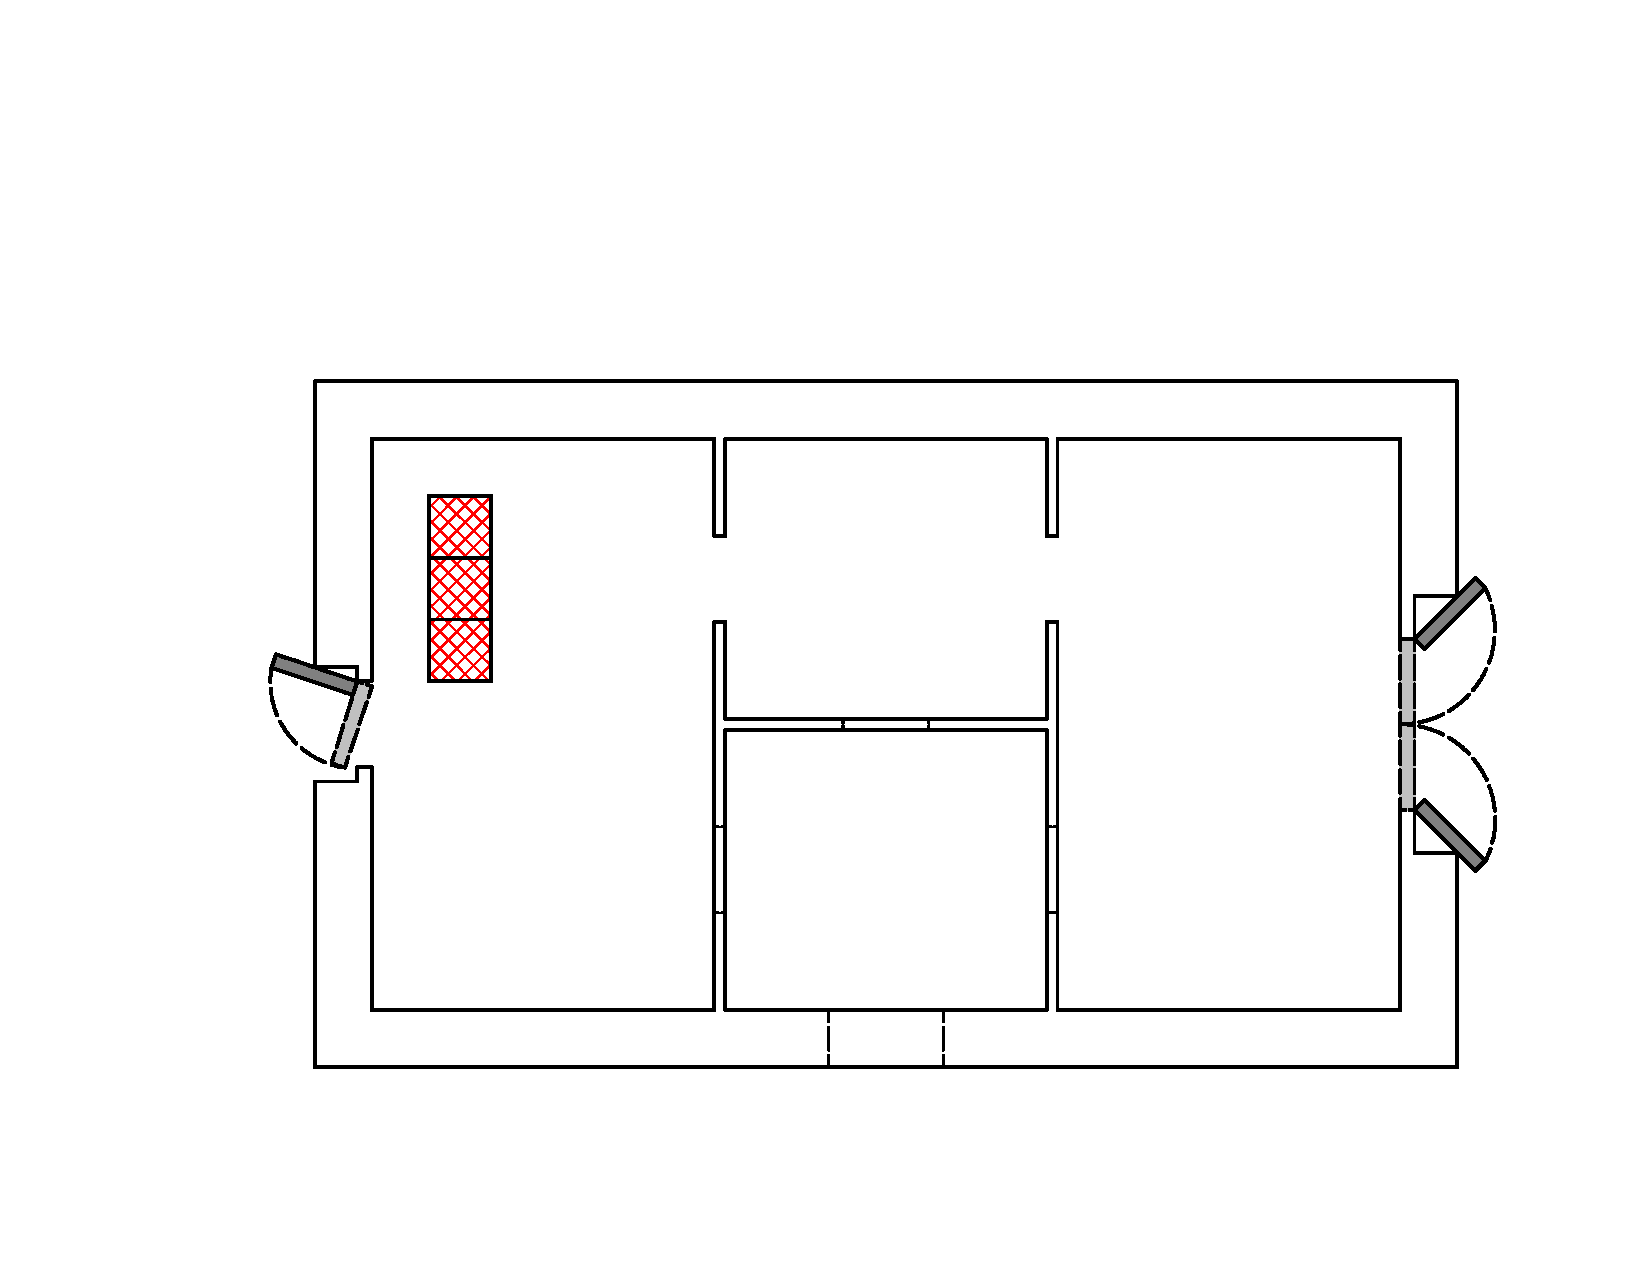
\includegraphics[width=\columnwidth]{../Figures/Floor_Plans/East_Structure_Test_4}
\end{minipage}
\caption{Tests~2-4 layout and event times.}
\label{fig:Tests_2-4_layout}
\end{figure}
\clearpage

\subsection{Tests 5 \& 6}
The procedures for Test~5 and Test~6 are outlined in Fig.~\ref{fig:east_test_5} and Fig.~\ref{fig:east_test_6}, respectively. Tests~5 and 6 involved repeating a specific set of events three times in a row. To avoid listing the identical actions three separate times in the event column of the table, each repetition of events has been denoted as a ``sequence'' (abbreviated as ``seq.'' in the tables) and given its own column in the event table. 

\begin{table}[!ht]
\caption{Heat Release Rates for Tests~5 and 6}
\begin{tabular}{lc}
 \toprule
 & \textbf{Heat Release Rate (kW)} \\
\textbf{Test} & \textbf{All Burners On} \\
\midrule
Test 5 - Seq. 1		& 1190 \\
Test 5 - Seq. 2		& 1190 \\
Test 5 - Seq. 3		& 1190 \\
Test 6 - Seq. 1		& 1190 \\
Test 6 - Seq. 2		& 1190 \\
Test 6 - Seq. 3		& 1180 \\
\bottomrule
\end{tabular}
\label{table:HRR_Tests_5-6}
\end{table}

\begin{figure}[!ht]
\begin{minipage}[b]{0.8\columnwidth}
	\begin{flushleft}
	\begin{tabular}{lccc}
	\multicolumn{4}{c}{\normalsize Event Times (s) for Test~5 Data File} \\
	\toprule
	\multicolumn{1}{c}{\textbf{Event}} 	& \textbf{Seq. 1} & \textbf{Seq. 2} & \textbf{Seq. 3} \\
	\midrule
	~(1)~ All burners on 				& 	0			  &	   1225			&	   2425		\\
	~(2)~ Roof vent opened 				&   154			  &    1345			&	   2545		\\
	~(3)~ West double door opened 		&	175			  &	   1432	 		&	   2632 	\\
	~(4)~ East double door opened 		&   361			  &    1524			&	   2730		\\
	~(5)~ Roof vent closed		 		&   445			  &    1723			&	   2852		\\
	~(6)~ All burners off 				&   576			  &    1840			&	   2997		\\
	~(7)~ Roof vent opened				& 	720 		  &	   1890			&	   3086		\\
	~(8)~ East double door closed		& 	1148 		  &	   2311			&	   N/A		\\
	~(9)~ West double door closed		& 	1164 		  &	   2330			&	   N/A		\\
	(10) Roof vent closed		 		&   1179		  &    2387			&	   N/A		\\
	\bottomrule
	\end{tabular}
	\end{flushleft}
\end{minipage}
\begin{minipage}[b]{0.9\columnwidth}
	\vspace{15pt}
	\centering
	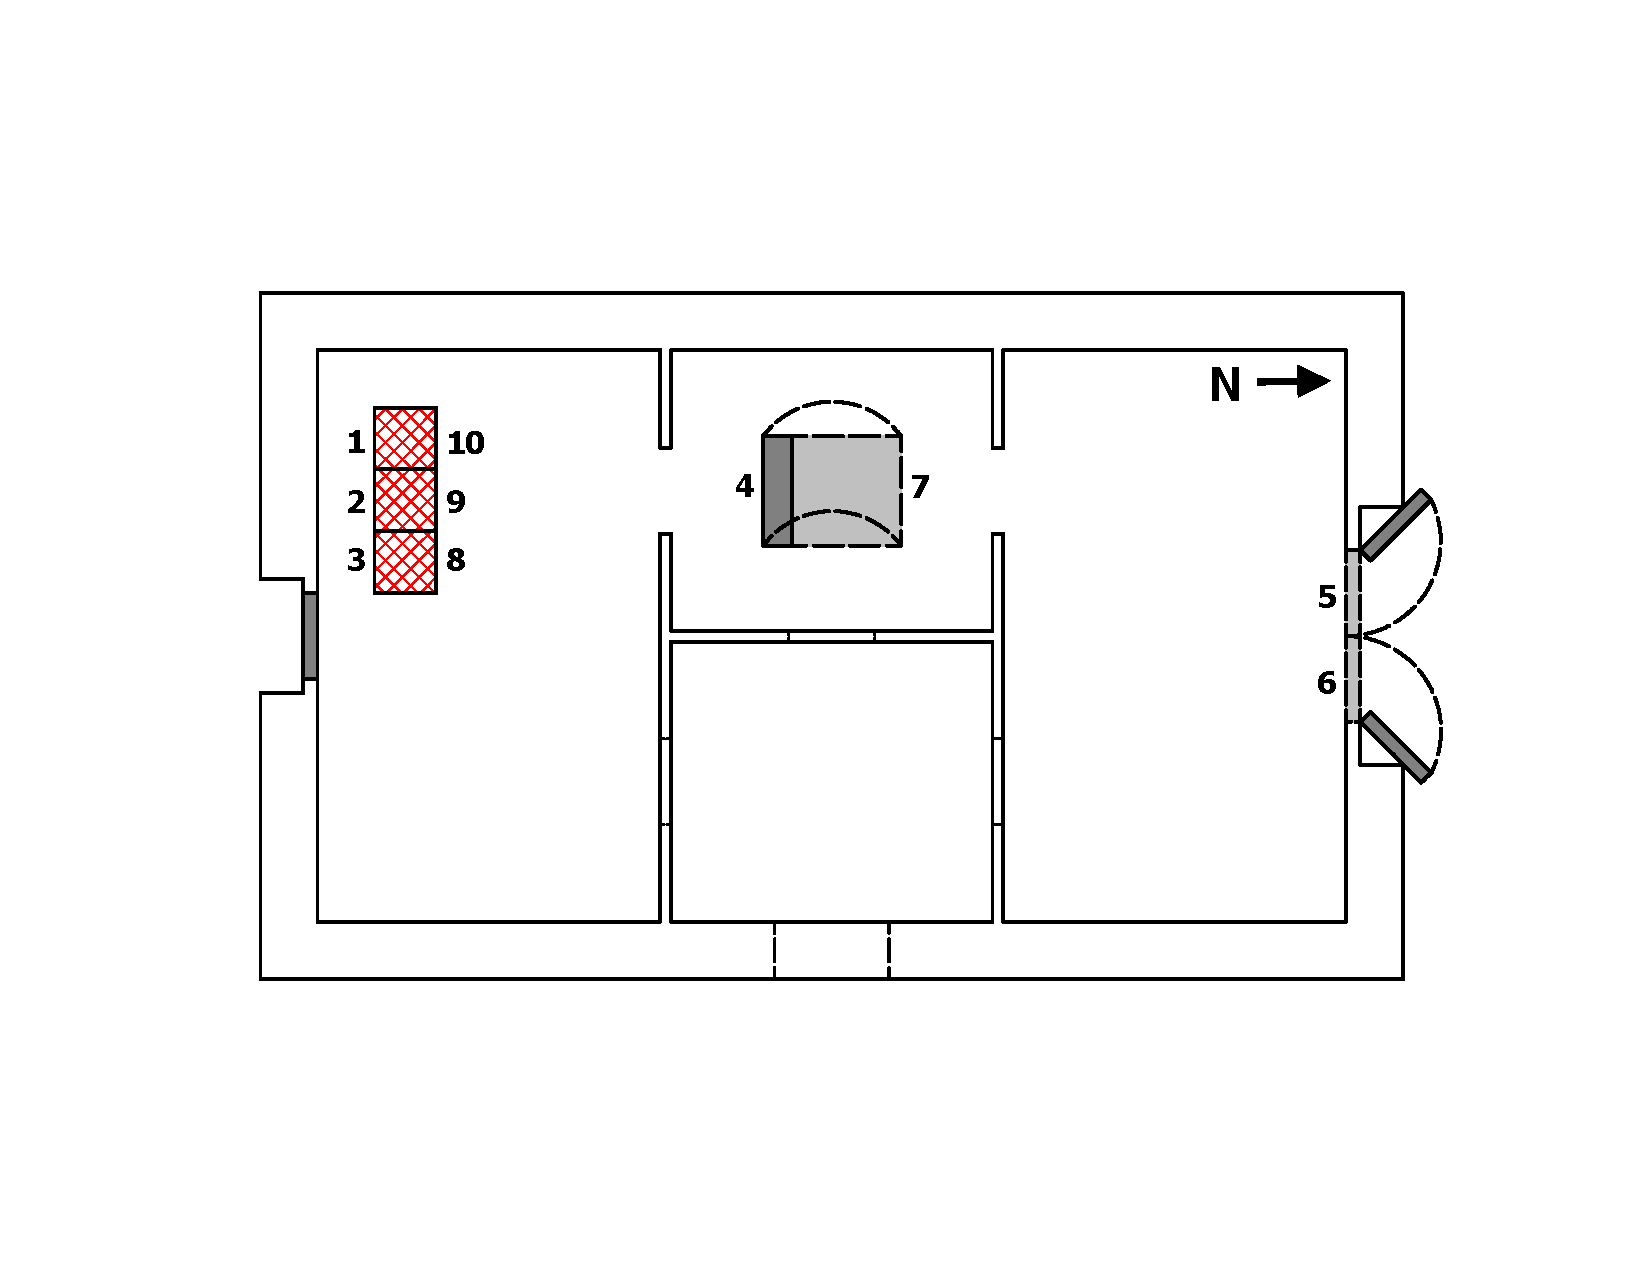
\includegraphics[width=0.86\columnwidth]{../Figures/Floor_Plans/East_Structure_Test_5}
\end{minipage}
\caption{Test~5 layout and event times.}
\label{fig:east_test_5}
\end{figure}

\begin{figure}[!ht]
\begin{minipage}[b]{0.8\columnwidth}
	\begin{flushleft}
	\begin{tabular}{lccc}
	\multicolumn{4}{c}{\normalsize Event Times (s) for Test~6 Data File} \\
	\toprule
	\multicolumn{1}{c}{\textbf{Event}} 	& \textbf{Seq. 1}	& \textbf{Seq. 2} 	& \textbf{Seq. 3} 	\\
	\midrule
	~(1)~ All burners on 				&	0				&	565				&	1075			\\
	~(2)~ West double door opened 		&	116				&   685				&	1195			\\
	~(3)~ Roof vent opened 		    	&	207				&	747 			& 	1287 			\\
	~(4)~ All burners off 				&	327				&   868				&	1387			\\
	~(5)~ East double door opened		&	369				&   911				&	1446			\\
	~(6)~ Roof vent closed 				&	494				&   1040			&	N/A				\\
	~(7)~ East double door closed		&	522 			&	1012			&	N/A 			\\
	~(8)~  West double door closed		&	538 			&	1025			&	N/A				\\
	\bottomrule
	\end{tabular}
	\end{flushleft}
\end{minipage}
\begin{minipage}[b]{0.86\columnwidth}
	\vspace{15pt}
	\centering
	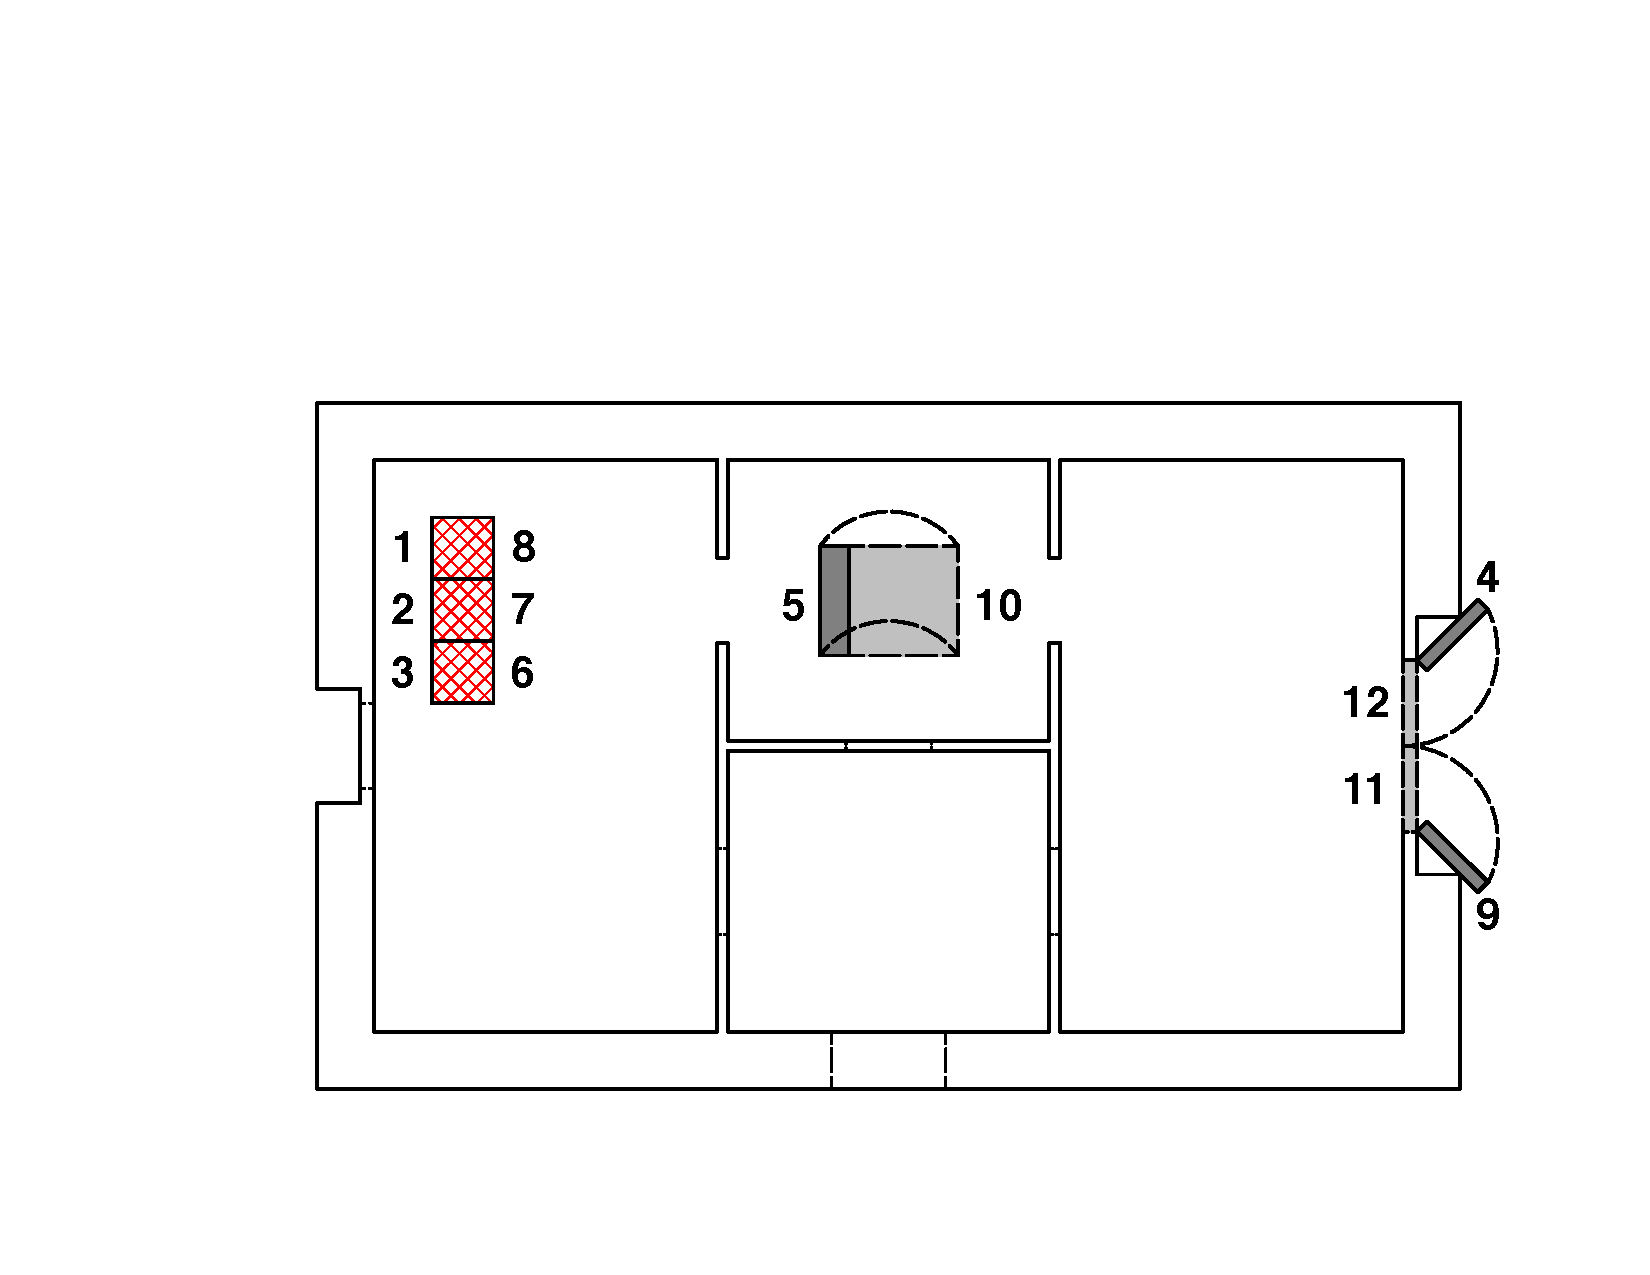
\includegraphics[width=\columnwidth]{../Figures/Floor_Plans/East_Structure_Test_6}
\end{minipage}
\caption{Test~6 layout and event times.}
\label{fig:east_test_6}
\end{figure}
\clearpage

\section{West Structure Tests}
\label{sec:west_procedure}
Four different tests, Tests~22--25, were conducted in the West Structure. Table~\ref{table:HRR_West} lists the calculated heat release rate for each test. Similar to Tests~5 and 6, Tests~22--25 had a duration on the order of seconds between the ignition of each burner, so only the heat release rate for when all three burners were ignited is reported.   

\begin{table}[!ht]
\caption{Heat Release Rates for West Structure Tests}
\begin{tabular}{lc}
 \toprule
					& 	\textbf{Heat Release Rate (kW)}	\\
\textbf{Test}		& All burners on \\
 \midrule
Test 22				&     	1240 	  \\
Test 23				&     	1290 	  \\
Test 24				& 	    1270 	  \\
Test 25				&     	1270 	  \\
\bottomrule
\end{tabular}
\label{table:HRR_West}
\end{table}

\subsection{Tests~22 \& 23}
Tests~22 and 23 followed an identical procedure to change the ventilation. Fig.~\ref{fig:west_test_22} includes a floor plan schematic and table of event times corresponding to the data files for Tests~22 and 23. A 61~cm (24~in) diameter PPV fan located 2.3~m (7.5~ft) away from the first level double doors and aimed at the center of the two doors was used during the tests to change the ventilation pattern within the structure.
\begin{figure}[!ht]
\begin{minipage}[b]{0.8\columnwidth}
	\begin{flushleft}
	\begin{tabular}{lcc}
	\multicolumn{3}{c}{Event Times (s) for Tests~22--23 Data Files} \\
	\toprule
	\multicolumn{1}{c}{\textbf{Event}} 			& \textbf{Test 22}	& \textbf{Test 23} \\
	\midrule
	~(1)~  All burners on 						&   0	  			&	 0			\\
	~(2)~  2nd floor west double door opened 	&   194		  		&    130		\\
	~(3)~  1st floor west double door opened 	&	314		  		&    252 	 	\\
	~(4)~  1st floor east double door opened 	&   450			  	&    371		\\
	~(5)~  2nd floor south exterior door closed &   511		  		&    N/A		\\
	~(6)~  2nd floor east double door opened	&   585			  	&    498		\\
	~(7)~  PPV fan on 							&   652			  	&    612		\\
	~(8)~  PPV fan off              			&   798			  	&    761		\\
	~(9)~  All burners off 						&   829			  	&    794		\\
	(10)   2nd floor south exterior door opened &   899			  	&    849		\\
	(11)   PPV fan on 	 						&   1065		  	&    940		\\
	(12)   2nd floor south exterior door closed &   1176		  	&    N/A		\\
	\bottomrule
	\end{tabular}
	\end{flushleft}
\end{minipage}
\begin{minipage}[b]{0.9\columnwidth}
	\vspace{15pt}
	\centering
	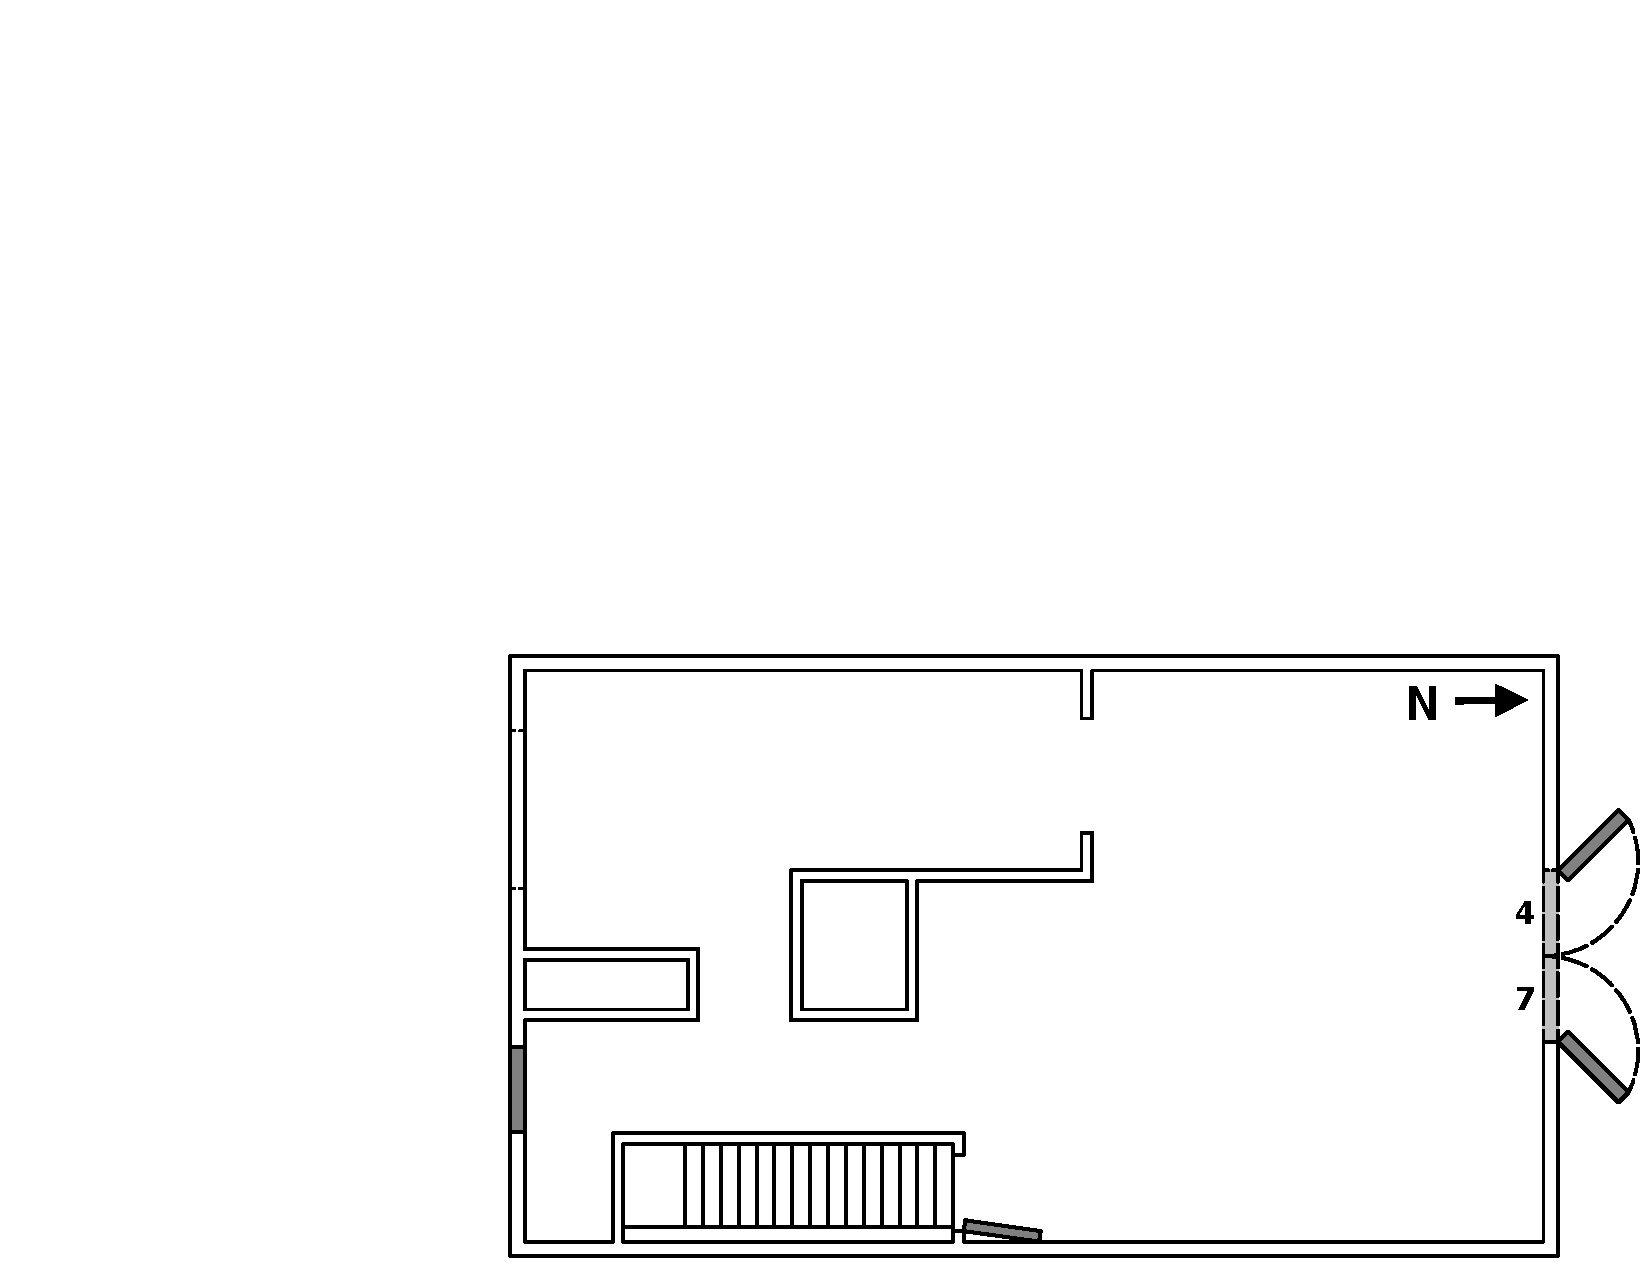
\includegraphics[width=\columnwidth]{../Figures/Floor_Plans/West_Structure_2nd_Floor_Test_22}
	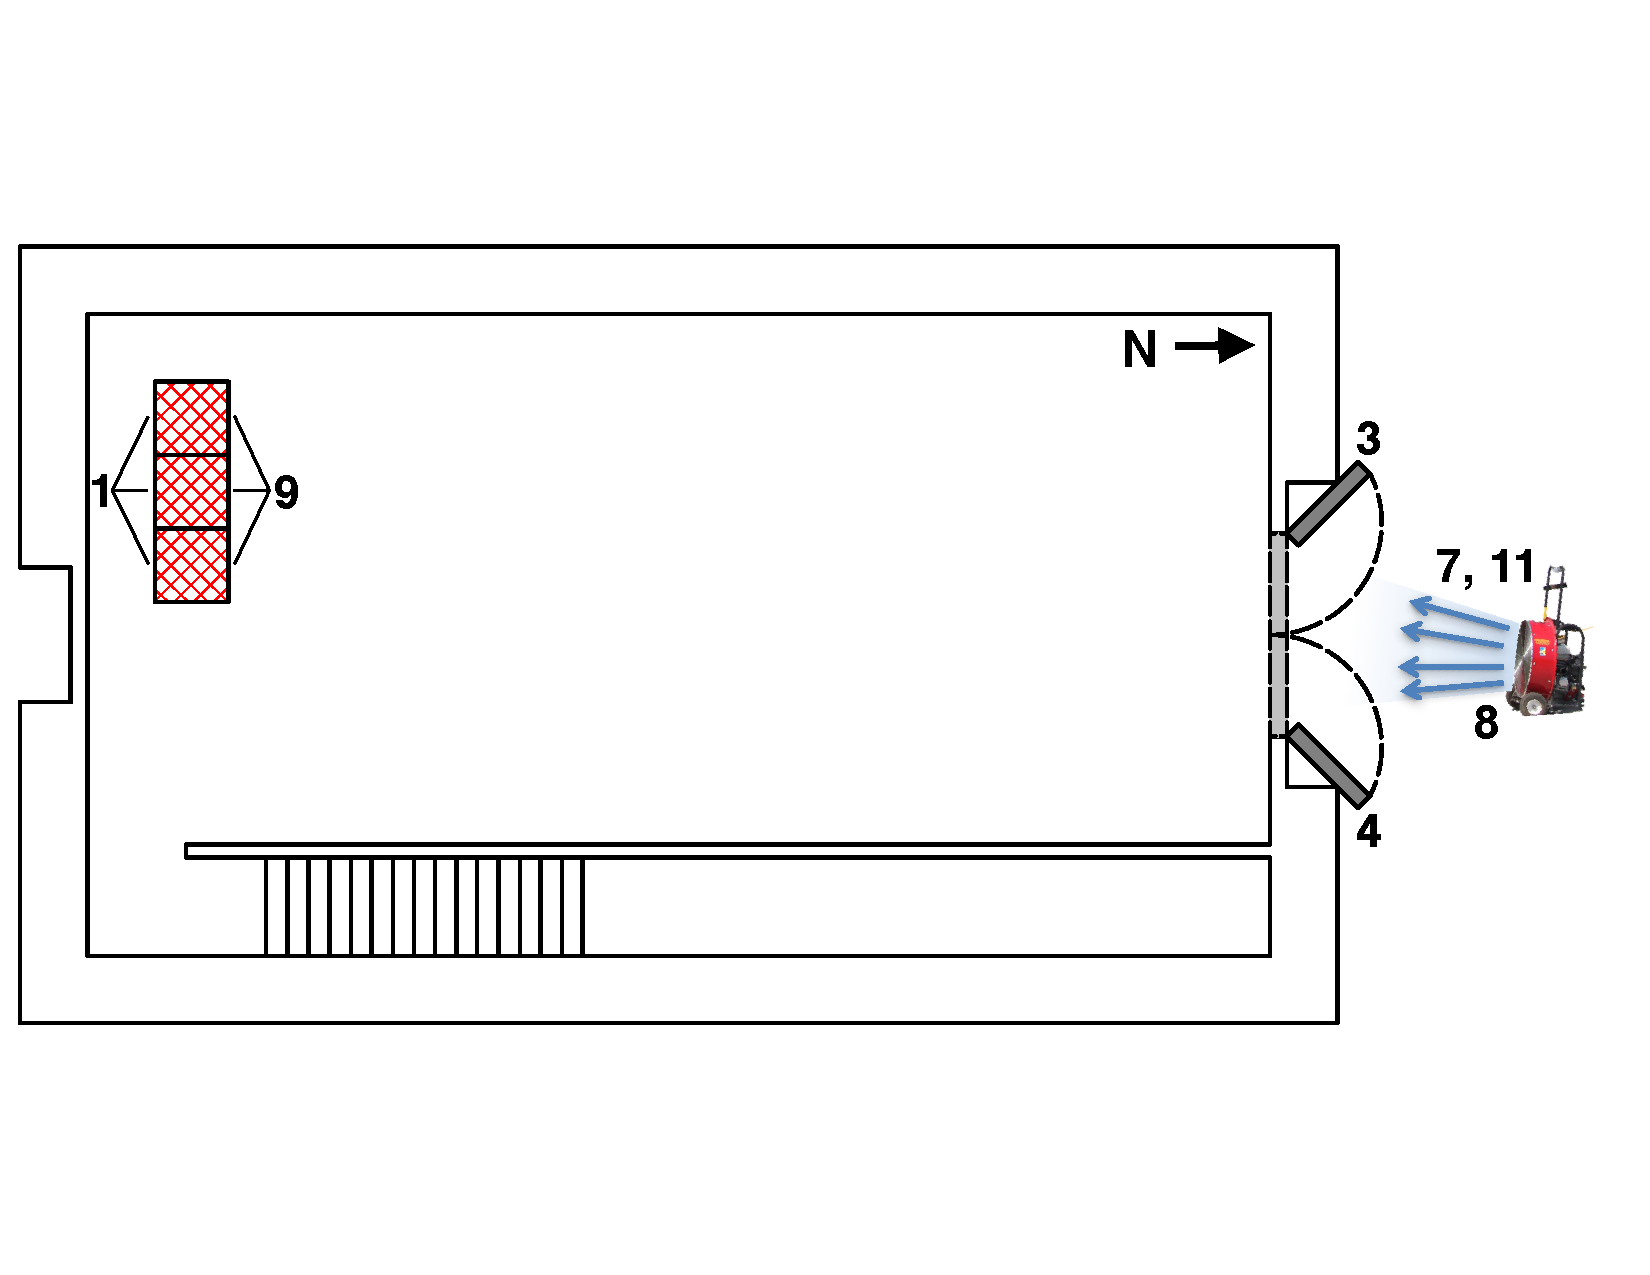
\includegraphics[width=0.98\columnwidth]{../Figures/Floor_Plans/West_Structure_1st_Floor_Test_22}
\end{minipage}
\caption{Tests 22--23 layout and event times.}
\label{fig:west_test_22}
\end{figure}

\subsection{Tests~24 \& 25}
Similar to Tests~22 and 23, Tests~24 and 25 followed an identical procedure to change the ventilation. Fig.~\ref{fig:west_test_24} includes a floor plan schematic and table of event times corresponding to the data files for Tests~24 and 25. A 61~cm (24~in) diameter PPV fan located 2.3~m (7.5~ft) away from the first level double doors and aimed at the center of the west double door was used during the tests to change the ventilation pattern within the structure. Also, the stairwell door was unable to completely close. So, when it was in the ``closed'' position at the beginning of the tests, there was a 152~mm (6~in) gap between the door and its frame. 

\begin{figure}[!ht]
\begin{minipage}[b]{0.8\columnwidth}
	\begin{flushleft}
	\begin{tabular}{lcc}
	\multicolumn{3}{c}{Event Times (s) for Tests 24--25 Data Files} \\
	\toprule
	\multicolumn{1}{c}{\textbf{Event}} 			& \textbf{Test 24}	& \textbf{Test 25} \\
	\midrule
	~(1)~ All burners on 						&   0		  		&	 0			\\
	~(2)~ Interior stairwell door opened 		&   144		  		&    112		\\
	~(3)~ 1st floor west double door opened 	&	265		  		&    244 	 	\\
	~(4)~ 2nd floor west double door opened 	&   383			  	&    353		\\
	~(5)~ 2nd floor south exterior door closed	&   452			  	&    N/A		\\
	~(6)~ 2nd floor south exterior door opened	&   502			  	&    474		\\
	~(7)~ PPV fan on 							&   624			  	&    594 		\\
	~(8)~ All burners off 						&   746 		  	&    721		\\
	~(9)~ 2nd floor east double door opened 	&   877			  	&    N/A		\\
	(10)  1st floor east double door opened		& 	N/A 			& 	 836		\\
	\bottomrule
	\end{tabular}
	\end{flushleft}
\end{minipage}
\begin{minipage}[b]{0.9\columnwidth}
	\vspace{15pt}
	\centering
	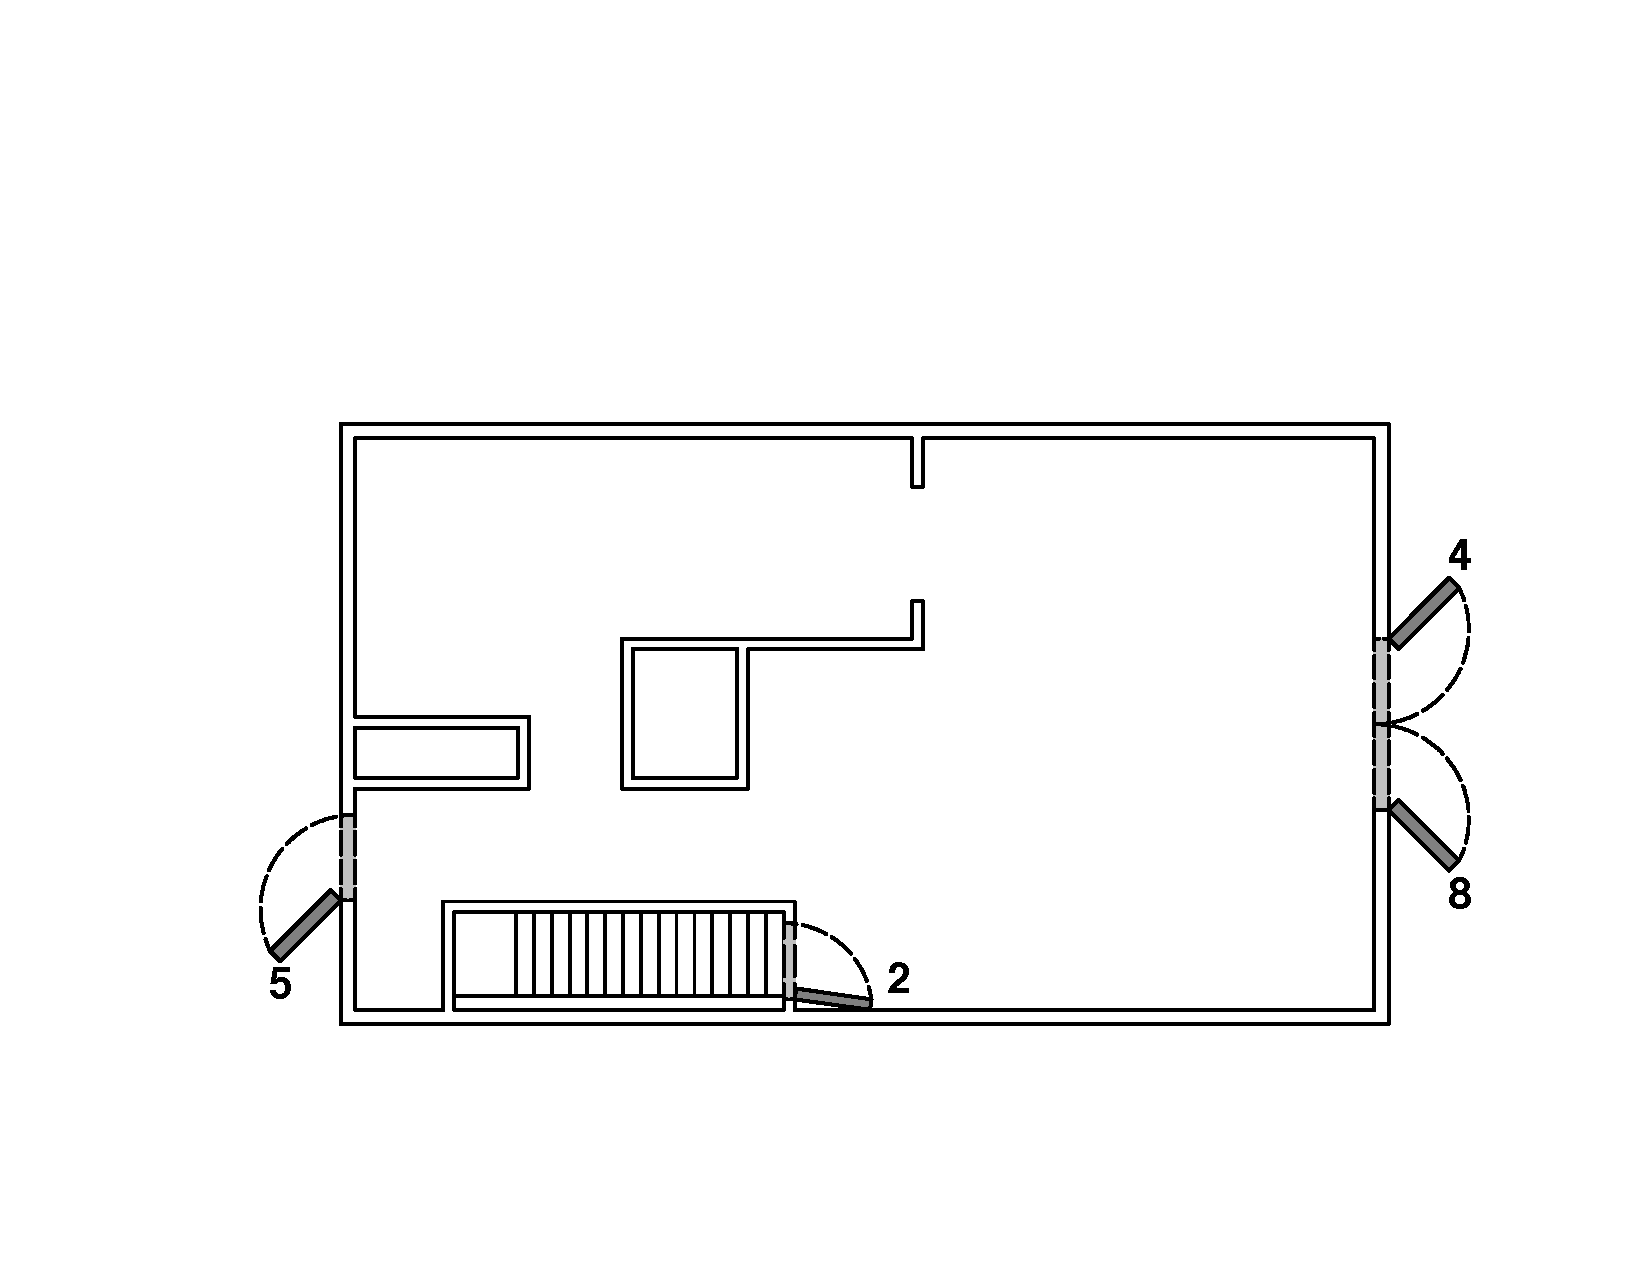
\includegraphics[width=\columnwidth]{../Figures/Floor_Plans/West_Structure_2nd_Floor_Test_24}
	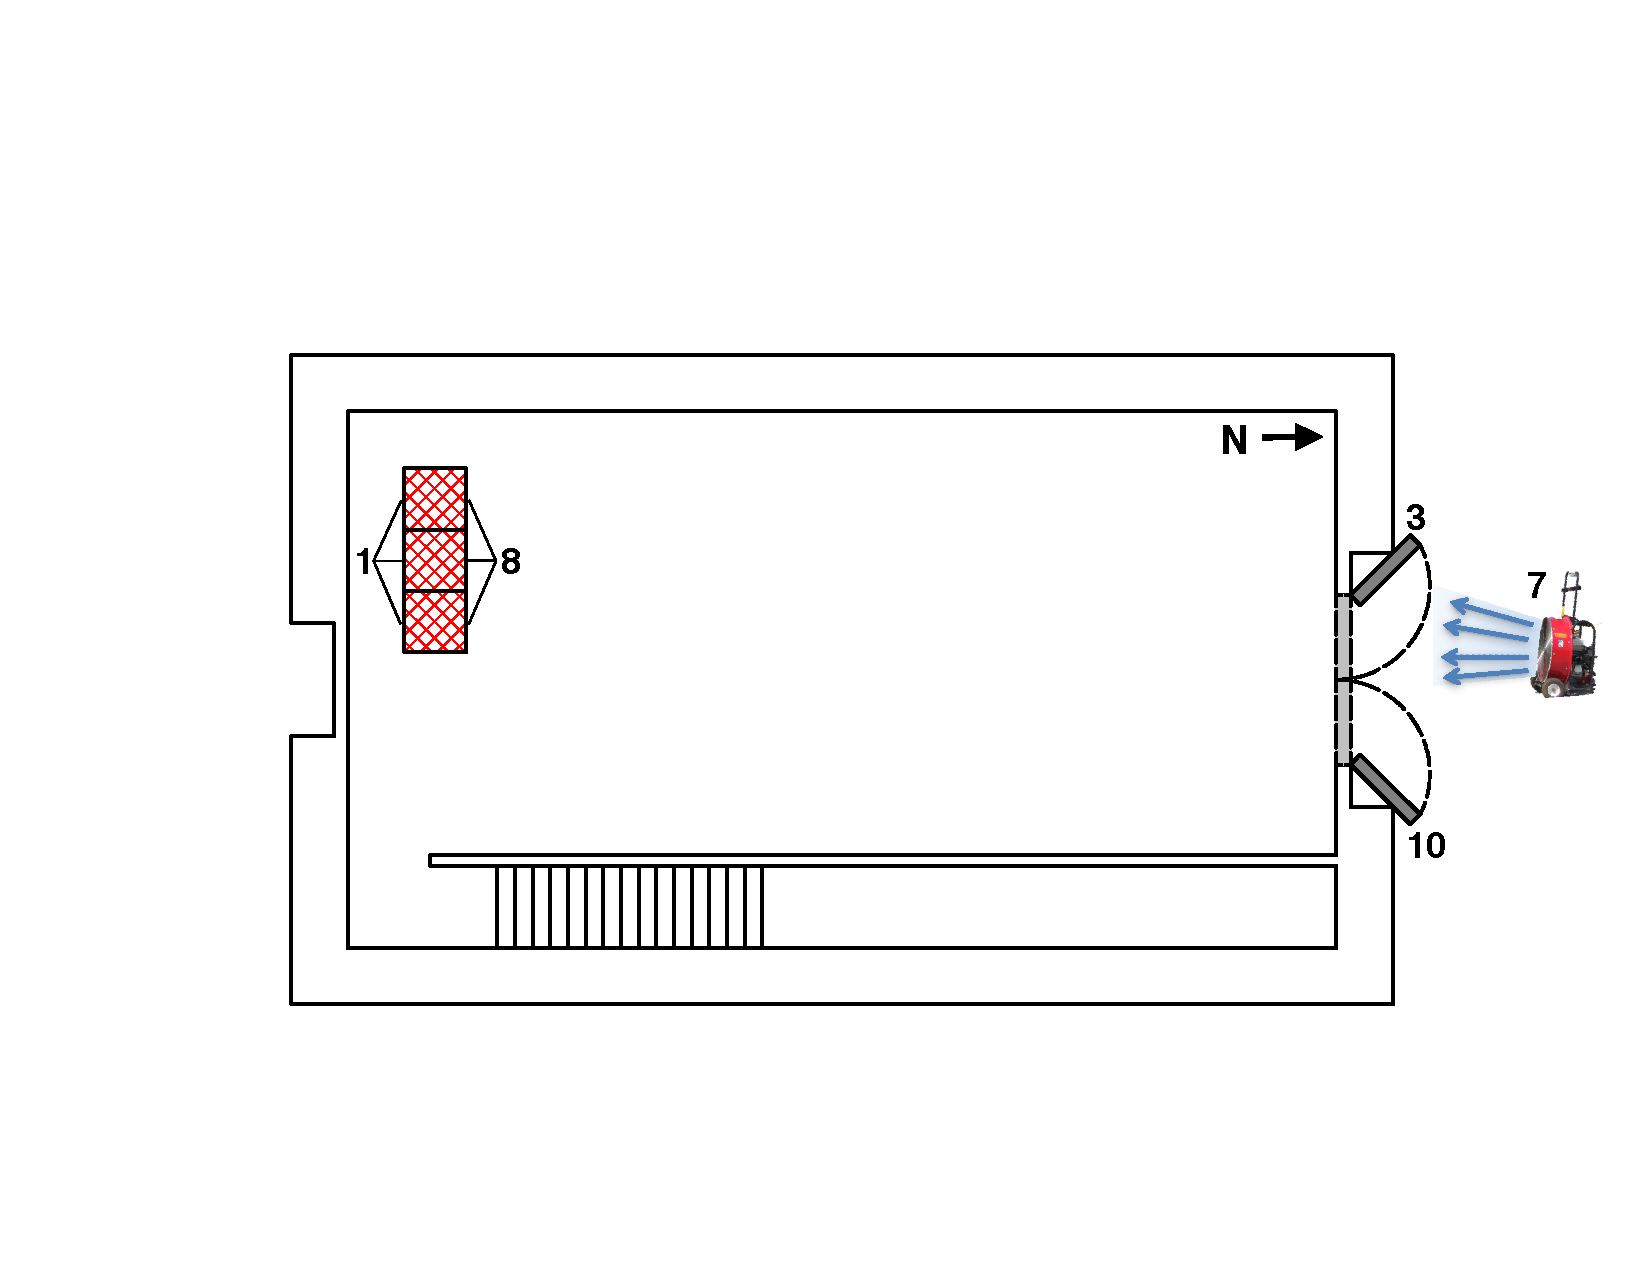
\includegraphics[width=0.97\columnwidth]{../Figures/Floor_Plans/West_Structure_1st_Floor_Test_24}
\end{minipage}
\caption{Tests 24--25 layout and event times.}
\label{fig:west_test_24}
\end{figure}
\clearpage

\chapter{Summary}
\label{chap:Summary}
Nine full-scale fire tests were conducted in two residential-sized structures to examine how changing ventilation patterns within a structure affects the fire environment. The fire source for each experiment was provided by a set of three diffusion flame burners with propane as the fuel. Various doors and vents were opened and closed during each test to affect the ventilation within the structure. A PPV fan was also used during some of the experiments to change the ventilation patterns. Local measurements of temperature, gas velocity, heat flux, and gas concentrations were collected at various locations throughout the structure during each experiment. The total volume of propane delivered to the burners was measured by a rotary gas meter and was used to calculate the heat release rate of the fire for each test.    

\bibliography{../../../../../Bibliography/FDS_refs,../../../../../Bibliography/FDS_general}

\appendix

\end{document}
